%%%%%%%%%%%%%%%%%%%%%%%%%%%%%%%%%%%%%%%%%%%%%%%%%%%%%%%%%%%%%%%%%%%%
%% Run LaTeX on this file several times to get Table of Contents,
%% cross-references, and citations.

%% If you have font problems, you may edit the w-bookps.sty file
%% to customize the font names to match those on your system.

%% w-bksamp.tex. Current Version: Feb 16, 2012
%%%%%%%%%%%%%%%%%%%%%%%%%%%%%%%%%%%%%%%%%%%%%%%%%%%%%%%%%%%%%%%%
%
%  Sample file for
%  Wiley Book Style, Design No.: SD 001B, 7x10
%  Wiley Book Style, Design No.: SD 004B, 6x9
%
%
%  Prepared by Amy Hendrickson, TeXnology Inc.
%  http://www.texnology.com
%%%%%%%%%%%%%%%%%%%%%%%%%%%%%%%%%%%%%%%%%%%%%%%%%%%%%%%%%%%%%%%%

%%%%%%%%%%%%%
% 7x10
%\documentclass{wileySev}

% 6x9
\documentclass{wileySix}

\usepackage{graphicx}
\usepackage{listings}
\usepackage{float}
\usepackage{url}


\usepackage{color}

\definecolor{codegreen}{rgb}{0,0.6,0}
\definecolor{codegray}{rgb}{0.5,0.5,0.5}
\definecolor{codepurple}{rgb}{0.58,0,0.82}
\definecolor{backcolour}{rgb}{0.95,0.95,0.92}

\lstdefinestyle{mystyle}{
    backgroundcolor=\color{backcolour},
    commentstyle=\color{codegreen},
    keywordstyle=\color{magenta},
    numberstyle=\tiny\color{codegray},
    stringstyle=\color{codepurple},
    basicstyle=\footnotesize,
    breakatwhitespace=false,
    breaklines=true,
    captionpos=b,
    keepspaces=true,
    numbers=left,
    numbersep=5pt,
    showspaces=false,
    showstringspaces=false,
    showtabs=false,
    tabsize=2,
    language=sh
}

\lstset{style=mystyle}

%%%%%%%
%% for times math: However, this package disables bold math (!)
%% \mathbf{x} will still work, but you will not have bold math
%% in section heads or chapter titles. If you don't use math
%% in those environments, mathptmx might be a good choice.

% \usepackage{mathptmx}

% For PostScript text
\usepackage{w-bookps}

%%%%%%%%%%%%%%%%%%%%%%%%%%%%%%%%%%%%%%%%%%%%%%%%%%%%%%%%%%%%%%%%
%% Other packages you might want to use:

% for chapter bibliography made with BibTeX
% \usepackage{chapterbib}

% for multiple indices
% \usepackage{multind}

% for answers to problems
% \usepackage{answers}

%%%%%%%%%%%%%%%%%%%%%%%%%%%%%%
%% Change options here if you want:
%%
%% How many levels of section head would you like numbered?
%% 0= no section numbers, 1= section, 2= subsection, 3= subsubsection
%%==>>
\setcounter{secnumdepth}{3}

%% How many levels of section head would you like to appear in the
%% Table of Contents?
%% 0= chapter titles, 1= section titles, 2= subsection titles,
%% 3= subsubsection titles.
%%==>>
\setcounter{tocdepth}{2}

%% Cropmarks? good for final page makeup
%% \docropmarks

%%%%%%%%%%%%%%%%%%%%%%%%%%%%%%
%
% DRAFT
%
% Uncomment to get double spacing between lines, current date and time
% printed at bottom of page.
% \draft
% (If you want to keep tables from becoming double spaced also uncomment
% this):
% \renewcommand{\arraystretch}{0.6}
%%%%%%%%%%%%%%%%%%%%%%%%%%%%%%

%%%%%%% Demo of section head containing sample macro:
%% To get a macro to expand correctly in a section head, with upper and
%% lower case math, put the definition and set the box
%% before \begin{document}, so that when it appears in the
%% table of contents it will also work:

\newcommand{\VT}[1]{\ensuremath{{V_{T#1}}}}

%% use a box to expand the macro before we put it into the section head:

\newbox\sectsavebox
\setbox\sectsavebox=\hbox{\boldmath\VT{xyz}}

%%%%%%%%%%%%%%%%% End Demo


\begin{document}


\booktitle{SIG (Sistem Informasi Geografis)}
\subtitle{Semester 5}

\authors{D4TI3A\\
\affil{Angkatan 2017}
%Floyd J. Fowler, Jr.\\
%\affil{University of New Mexico}
}

\offprintinfo{SIG (Sistem Informasi Geografis), First Edition}{D4TI3A}

%% Can use \\ if title, and edition are too wide, ie,
%% \offprintinfo{Survey Methodology,\\ Second Edition}{Robert M. Groves}

%%%%%%%%%%%%%%%%%%%%%%%%%%%%%%
%%
\halftitlepage

%\titlepage


\begin{copyrightpage}{2019}
\input{info/copyrightpage}
\end{copyrightpage}

\dedication{`Jika Kamu tidak dapat menahan lelahnya belajar,
Maka kamu harus sanggup menahan perihnya Kebodohan.'
~Imam Syafi'i~}

\begin{contributors}
\input{info/contributors}
\end{contributors}

\contentsinbrief
\tableofcontents
\listoffigures
\listoftables
\lstlistoflistings


\begin{foreword}
\input{info/foreword}
\end{foreword}

\begin{preface}
\input{info/preface}
\end{preface}


\begin{acknowledgments}
\input{info/acknowledgments}
\end{acknowledgments}

\begin{acronyms}
\input{info/acronyms}
\end{acronyms}

\begin{glossary}
\input{info/glossary}
\end{glossary}

\begin{symbols}
\input{info/symbols}
\end{symbols}

\begin{introduction}
\input{info/introduction}
\end{introduction}

%%%%%%%%%%%%%%%%%% Isi Buku %%%%%%%%%%%%%%%%%%
\chapter{Tugas Pertama}
\input{chapters/tugas1/1174xxx}
\section{D. Irga B. Naufal Fakrhi (1174066)}
\subsection{LeafletJS dan MapProxy}
\begin{enumerate}
    \item Jalankan terlebih dahulu mapproxy pada folder gede dengan menggunakan setingan agm.yaml
        \hfill\break
        \begin{figure}[H]
        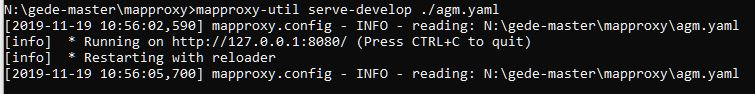
\includegraphics[width=4cm]{figures/tugas5/1174066/1.jpg}
        \centering
        \caption{Menjalankan Mapproxy}
        \end{figure}
    \item Setelah itu buka file basic.html pada folder leafletjs yang ada di dalam folder gede menggunakan browser
        \hfill\break
        \begin{figure}[H]
        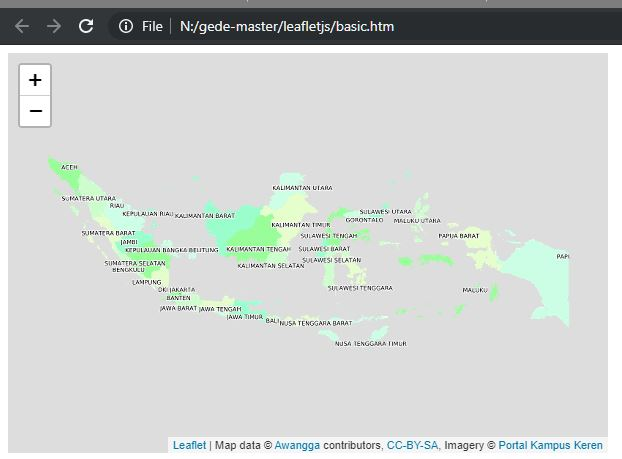
\includegraphics[width=4cm]{figures/tugas5/1174066/3.jpg}
        \centering
        \caption{Hasil dari file basic.htm}
        \end{figure}
   \item Dengan menggunakan LeafletJS kita dapat menambahkan marker, circle dan polygon yaitu dengan cara seperti gambar dibawah ini yang ada pada file marker.html pada folder gede/leafletjs
        \hfill\break
        \begin{figure}[H]
        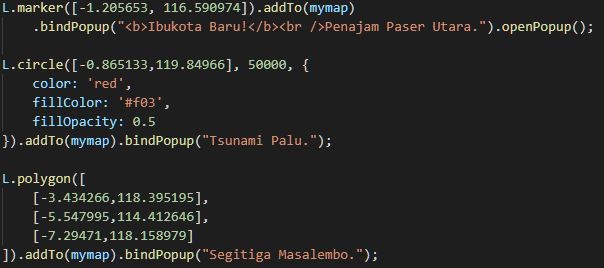
\includegraphics[width=4cm]{figures/tugas5/1174066/4.jpg}
        \centering
        \caption{Contoh menambahkan marker, circle dan polygon}
        \end{figure}
   \item Apabila file tersebut dibuka di browser maka akan muncul seperti ini
        \hfill\break
        \begin{figure}[H]
        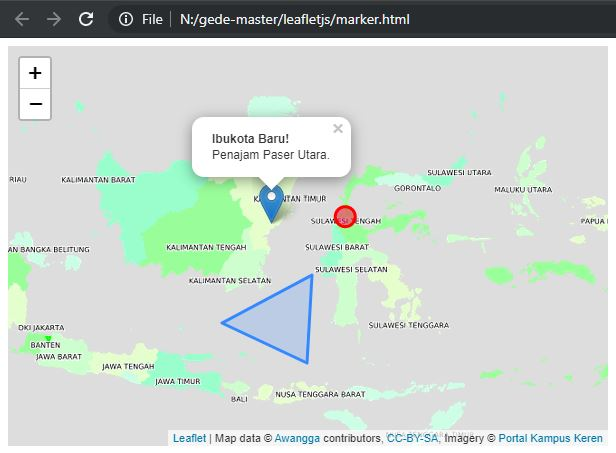
\includegraphics[width=4cm]{figures/tugas5/1174066/5.jpg}
        \centering
        \caption{Hasil dari file marker.html}
        \end{figure}
\end{enumerate}
\subsection{Link Youtube LeafletJS dan MapProxy}
https://youtu.be/cW\_TD69y62U

\section{Chandra Kirana Poetra (1174079)}
\subsection{Menggunakan LeafletJS dengan MapProxy}
\begin{enumerate}
    \item Jalankan dulu mapproxy yang kemarin telah dibuat di gede-master
    \hfill\break
    \begin{figure}[H]
		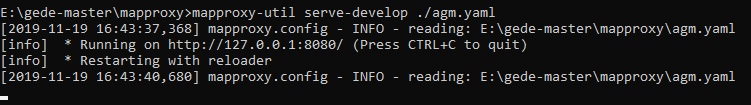
\includegraphics[width=12cm]{figures/Tugas5/1174079/1.png}
		\centering
		\caption{Gambar 1}
	\end{figure}
    \item Buka file basic.html di folder LeafletJS di dalam folder gede
    \hfill\break
    \begin{figure}[H]
		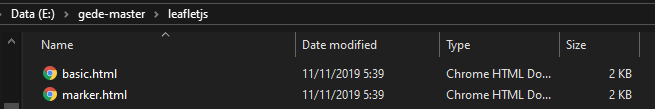
\includegraphics[width=12cm]{figures/Tugas5/1174079/2.png}
		\centering
		\caption{Gambar 2}
	\end{figure}
    \item Berikut adalah hasil dari file basic.html
    \hfill\break
    \begin{figure}[H]
		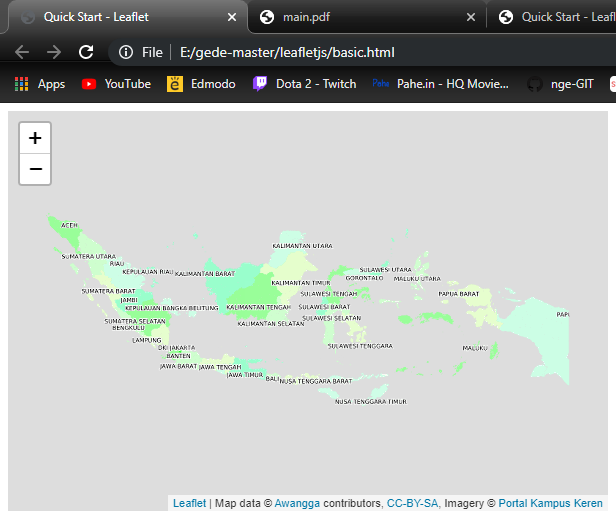
\includegraphics[width=12cm]{figures/Tugas5/1174079/3.png}
		\centering
		\caption{Gambar 3}
	\end{figure}
    \item Di leafletjs kita juga bisa menambahkan penanda atau marker,circle, ataupun polygon sebagai penanda dengan cara seperti di gambar
    \hfill\break
    \begin{figure}[H]
		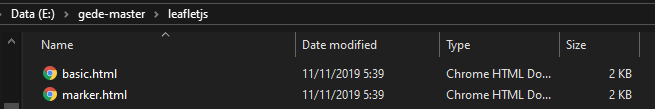
\includegraphics[width=12cm]{figures/Tugas5/1174079/2.png}
		\centering
		\caption{Gambar 4}
	\end{figure}
	\begin{figure}[H]
		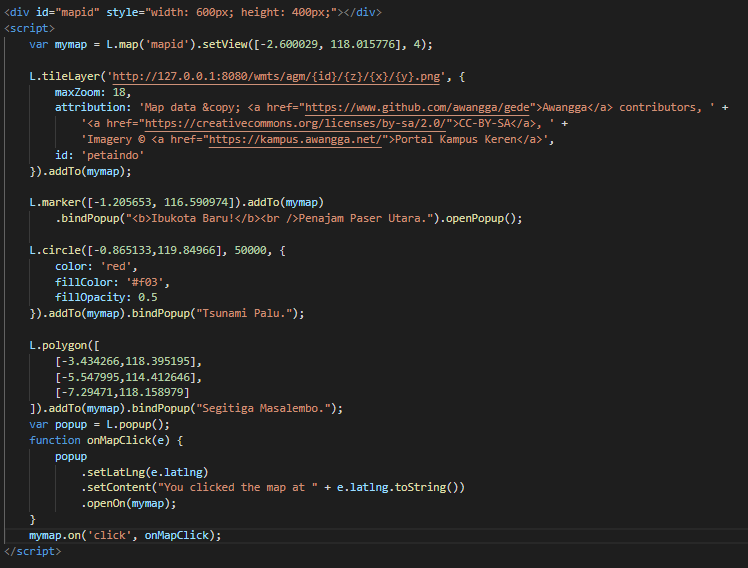
\includegraphics[width=12cm]{figures/Tugas5/1174079/4.png}
		\centering
		\caption{Gambar 5}
	\end{figure}
    \item Lalu coba buka di browser
    \hfill\break
    \begin{figure}[H]
		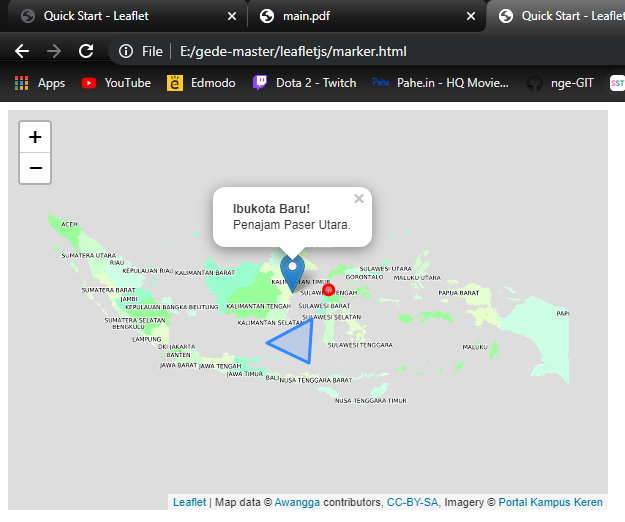
\includegraphics[width=12cm]{figures/Tugas5/1174079/5.png}
		\centering
		\caption{Gambar 6}
	\end{figure}
\end{enumerate}
\subsection{Link Youtube}
https://youtu.be/0PGjQqv-Dec
\input{chapters/tugas1/1174089}
\section{Tia Nur Candida (1174086)}
\subsection{Menggunakan LeafletJS dengan MapProxy}
\begin{enumerate}
    \item Run terlebih dahulu Mapproxy
    \hfill\break
    \begin{figure}[H]
		
\includegraphics[width=12cm]{figures/Tugas5/1174086/1.png}
		\centering
		\caption{Gambar 1}
	\end{figure}
    \item Buka file basic.html di dalam folder leafletjs di dalam folder gede
    \hfill\break
    \begin{figure}[H]
		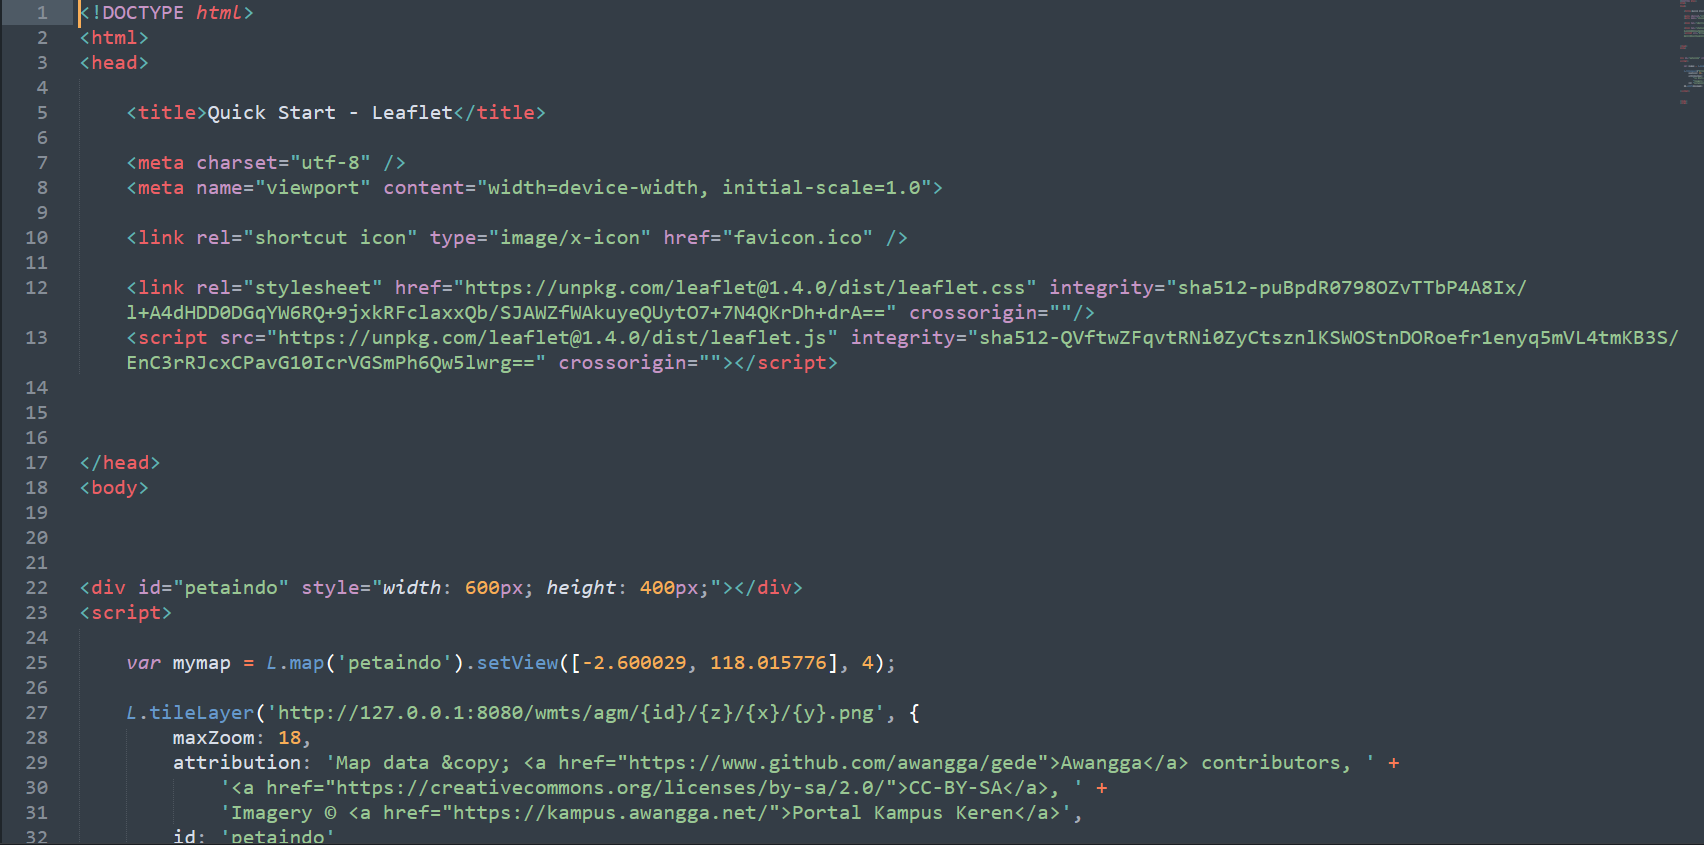
\includegraphics[width=12cm]{figures/Tugas5/1174086/3.png}
		\centering
		\caption{Gambar 2}
	\end{figure}
    \item Lalu buka file tersebut di browser, maka hasilnya akan seperti berikut
    \hfill\break
    \begin{figure}[H]
		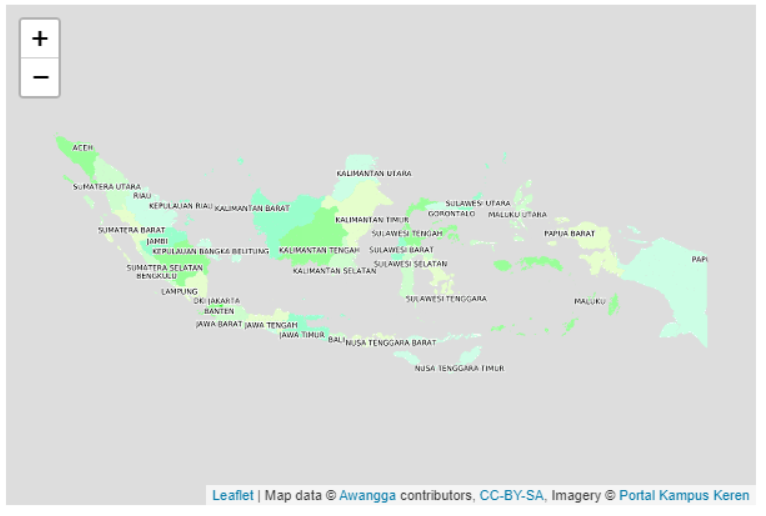
\includegraphics[width=12cm]{figures/Tugas5/1174086/4.png}
		\centering
		\caption{Gambar 3}
	\end{figure}
    \item Pada leafletjs dapat menambahkan marker,circle, ataupun polygon 
    \hfill\break
    \begin{figure}[H]
		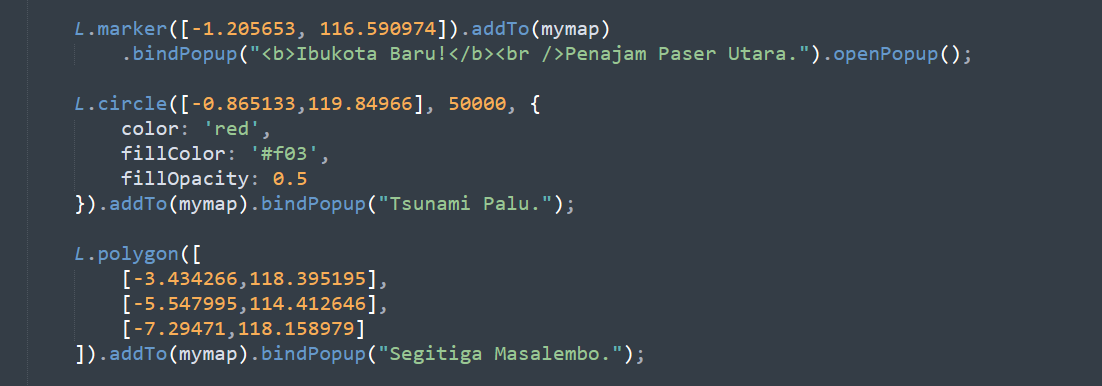
\includegraphics[width=12cm]{figures/Tugas5/1174086/5.png}
		\centering
		\caption{Gambar 4}
	\end{figure}
    \item Lalu buka file tersebut dengan browser dan hasilnya akan seperti berikut
    \hfill\break
    \begin{figure}[H]
		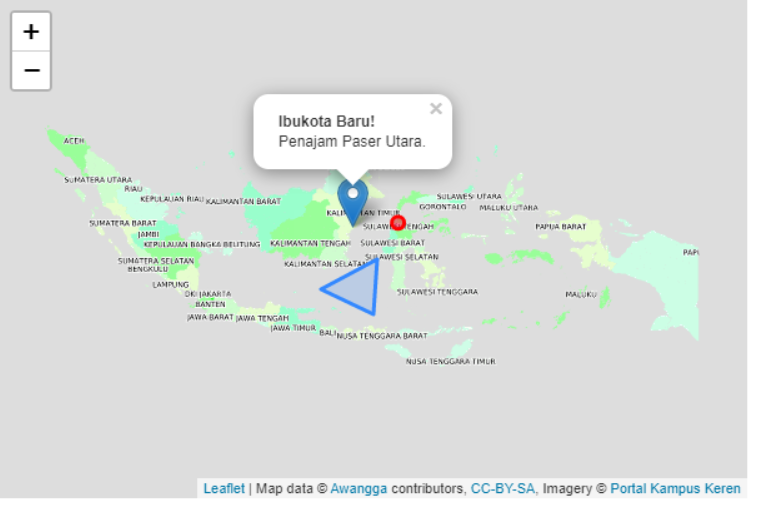
\includegraphics[width=12cm]{figures/Tugas5/1174086/6.png}
		\centering
		\caption{Gambar 5}
	\end{figure}
\end{enumerate}
\subsection{Link Youtube}
https://youtu.be/Qqu4UE9od9w
\section{Kaka Kamaludin (1174067)}
\subsection{LeafletJS dan MapProxy}
\begin{enumerate}
    \item Jalankan terlebih dahulu mapproxy pada folder gede dengan menggunakan setingan agm.yaml
        \hfill\break
        \begin{figure}[H]
        
\includegraphics[width=4cm]{figures/tugas5/1174067/1.png}
        \centering
        \caption{Menjalankan Mapproxy}
        \end{figure}
    \item Setelah itu buka file basic.html pada folder leafletjs yang ada di dalam folder gede menggunakan browser
        \hfill\break
        \begin{figure}[H]
        \includegraphics[width=4cm]{figures/tugas5/1174067/3.png}
        \centering
        \caption{Hasil dari file basic.htm}
        \end{figure}
   \item Dengan menggunakan LeafletJS kita dapat menambahkan marker, circle dan polygon yaitu dengan cara seperti gambar dibawah ini yang ada pada file marker.html pada folder gede/leafletjs
        \hfill\break
        \begin{figure}[H]
        \includegraphics[width=4cm]{figures/tugas5/1174067/4.png}
        \centering
        \caption{Contoh menambahkan marker, circle dan polygon}
        \end{figure}
   \item Apabila file tersebut dibuka di browser maka akan muncul seperti ini
        \hfill\break
        \begin{figure}[H]
        
\includegraphics[width=4cm]{figures/tugas5/1174067/5.png}
        \centering
        \caption{Hasil dari file marker.html}
        \end{figure}
\end{enumerate}
\subsection{Link Youtube LeafletJS dan MapProxy}
https://youtu.be/xJqh\_aY9Exk

\section{Fanny Shafira Damayanti (1174069)}
\subsection{LeafletJS dan Mapproxy}
\begin{enumerate}
    \item Langkah pertama yaitu run terlebih dahulu mapproxy nya.
  \hfill\break
  \begin{figure}[H]
  
\includegraphics[width=4cm]{figures/tugas5/1174069/1.png}
  \centering
  \caption{Run Mapproxy}
  \end{figure}
    
   

    \item Setelah itu buka contoh file leafletjs yang ada di dalam folder gede  yang telah kita download sebelumnya .
    
  \hfill\break
  \begin{figure}[H]
  
\includegraphics[width=4cm]{figures/tugas5/1174069/2.png}
  \centering
  \caption{Isi Basic.html}
  \end{figure}
    
    \item Kemudian buka browser, maka hasilnya akan seperti ini
    
  \hfill\break
  \begin{figure}[H]
  \includegraphics[width=4cm]{figures/tugas5/1174069/3.png}
  \centering
  \caption{Hasil dari Basic.html}
  \end{figure}
  
   \item Dengan menggunakan LeafletJS kita dapat menambhakan marker, circle dan polygon yaitu dengan cara seperti gambar dibawah ini, contoh ini diambil dari file marker.html yang berada didalam folder gerede.
    
  \hfill\break
  \begin{figure}[H]
  \includegraphics[width=4cm]{figures/tugas5/1174069/4.png}
  \centering
  \caption{Isi dari marker.html}
  \end{figure}
  
   \item kemudian buka filenya di browser, hasilnya seperti gambar dibawah ini.
  \hfill\break
  \begin{figure}[H]
  
\includegraphics[width=4cm]{figures/tugas5/1174069/5.png}
  \centering
  \caption{Isi dari marker.html}
  \end{figure}

\end{enumerate}

\subsection{Link Youtube MapProxy dan Menjalankannya}
\verb|https://youtu.be/j_zLb519AQ0|
\section{Ilham Muhammad Ariq(1174087)}
\subsection{Menggunakan LeafletJS dengan MapProxy}
\begin{enumerate}
    \item Kita run terlebih dahulu MapProxy yang telah dibuat kemarin yaitu agm.yaml
    \hfill\break
    \begin{figure}[H]
		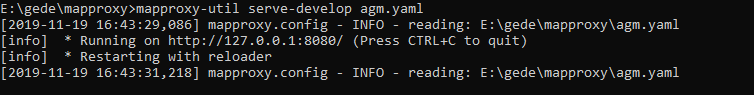
\includegraphics[width=12cm]{figures/Tugas5/1174087/1.png}
		\centering
		\caption{Start server MapProxy}
	\end{figure}
    \item Buka file contoh penggunaan LeafletJS yaitu basic.html di dalam folder leafletjs di dalam folder gede
    \hfill\break
    \begin{figure}[H]
		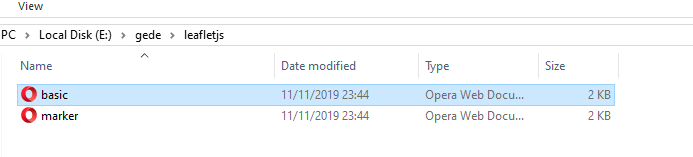
\includegraphics[width=12cm]{figures/Tugas5/1174087/2.png}
		\centering
		\caption{File Basic.html}
	\end{figure}
	\begin{figure}[H]
		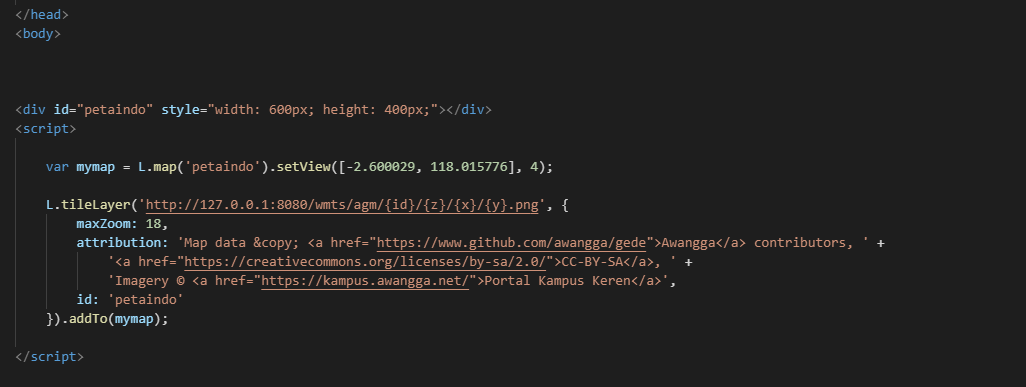
\includegraphics[width=12cm]{figures/Tugas5/1174087/7.png}
		\centering
		\caption{Code Basic.html}
	\end{figure}
    \item Lalu buka file tersebut di browser, maka hasilnya akan seperti ini
    \hfill\break
    \begin{figure}[H]
		\includegraphics[width=12cm]{figures/Tugas5/1174087/3.png}
		\centering
		\caption{Tampilan Basic.html}
	\end{figure}
    \item Dengan leafletjs kita juga dapat menambahkan marker,circle, ataupun polygon dengan cara menggunakan seperti di gambar, contoh ini diambil dari file contoh kedua yaitu marker.html dari folder gede 
    \hfill\break
    \begin{figure}[H]
		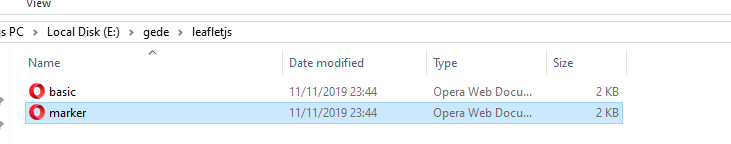
\includegraphics[width=12cm]{figures/Tugas5/1174087/4.png}
		\centering
		\caption{File Marker.html}
	\end{figure}
	\begin{figure}[H]
		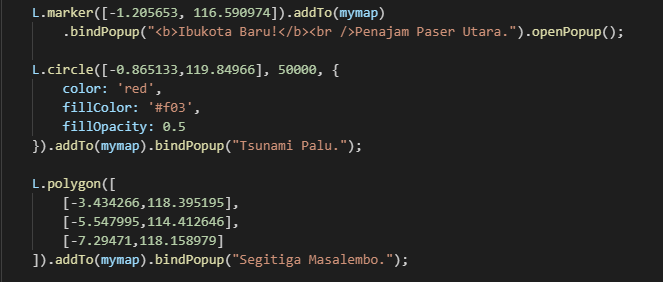
\includegraphics[width=12cm]{figures/Tugas5/1174087/6.png}
		\centering
		\caption{Code tambahan Marker.html}
	\end{figure}
    \item Lalu buka file tersebut dengan browser dan hasilnya akan seperti pada di gambar
    \hfill\break
    \begin{figure}[H]
		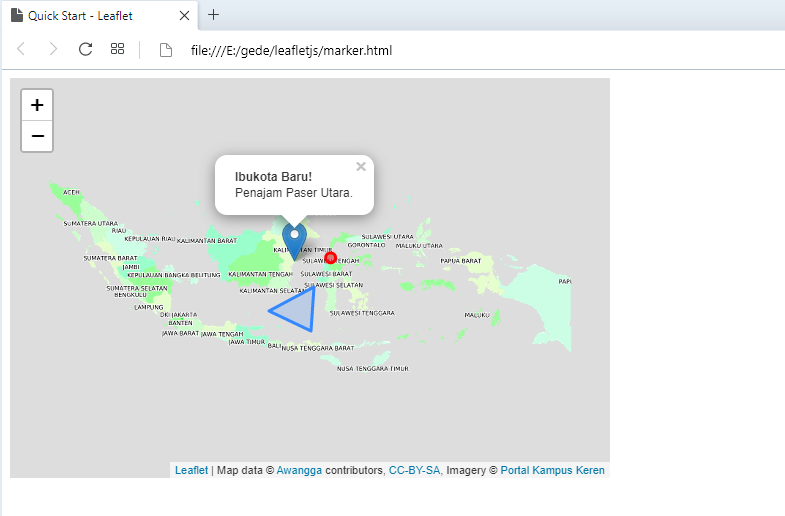
\includegraphics[width=12cm]{figures/Tugas5/1174087/5.png}
		\centering
		\caption{Tampilan Marker.html}
	\end{figure}
\end{enumerate}
\subsection{Link Youtube}
\verb|https://youtu.be/qANOELQ_0fE|
\section{Alvan Alvanzah (1174077)}
\subsection{Menggunakan LeafletJS dengan MapProxy}
\begin{enumerate}
    \item Kita run terlebih dahulu MapProxy yang telah dibuat kemarin yaitu agm.yaml
    \hfill\break
    \begin{figure}[H]
		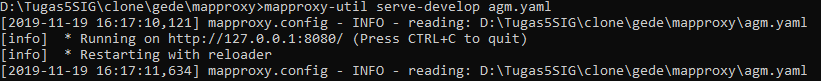
\includegraphics[width=12cm]{figures/Tugas5/1174077/1.png}
		\centering
		\caption{Start server MapProxy}
	\end{figure}
    \item Buka file contoh penggunaan LeafletJS yaitu basic.html di dalam folder leafletjs di dalam folder gede
    \hfill\break
    \begin{figure}[H]
		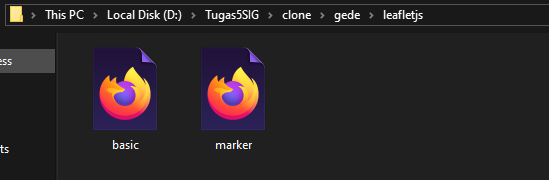
\includegraphics[width=12cm]{figures/Tugas5/1174077/2.png}
		\centering
		\caption{File Basic.html}
	\end{figure}
	\begin{figure}[H]
		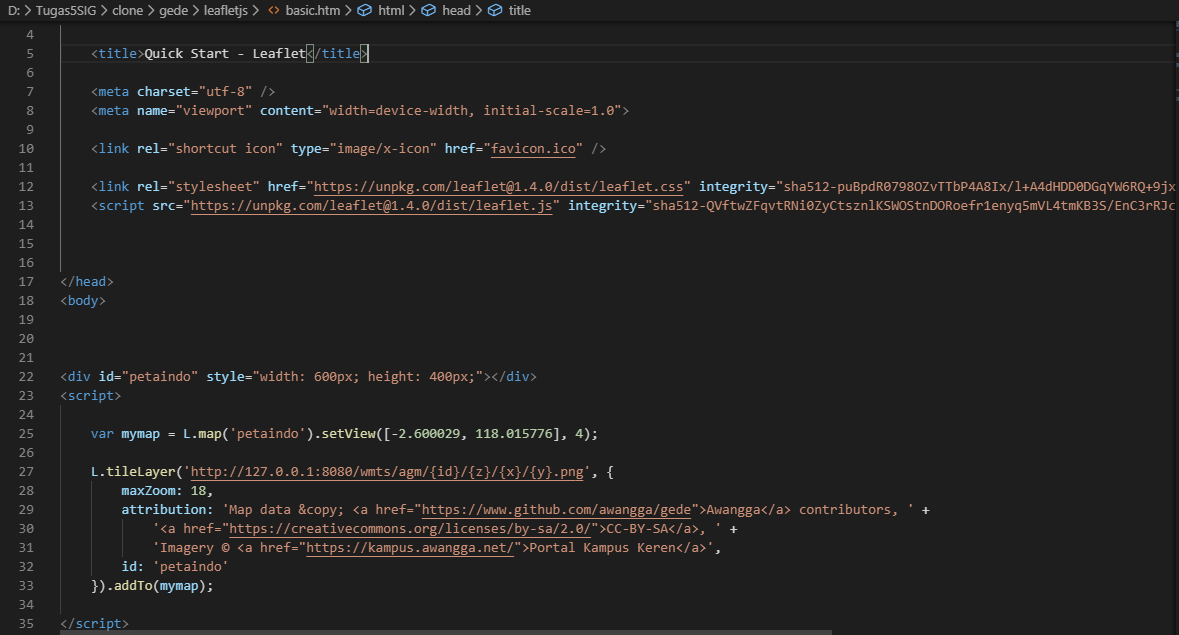
\includegraphics[width=12cm]{figures/Tugas5/1174077/7.png}
		\centering
		\caption{Code Basic.html}
	\end{figure}
    \item Lalu buka file tersebut di browser, maka hasilnya akan seperti ini
    \hfill\break
    \begin{figure}[H]
		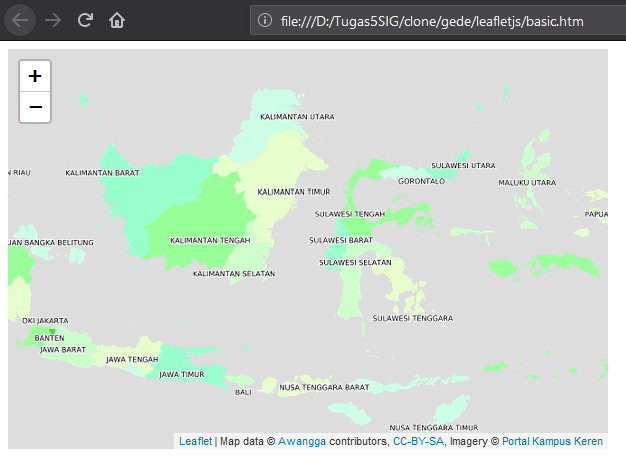
\includegraphics[width=12cm]{figures/Tugas5/1174077/3.png}
		\centering
		\caption{Tampilan Basic.html}
	\end{figure}
    \item Dengan leafletjs kita juga dapat menambahkan marker,circle, ataupun polygon dengan cara menggunakan seperti di gambar, contoh ini diambil dari file contoh kedua yaitu marker.html dari folder gede 
    \hfill\break
    \begin{figure}[H]
		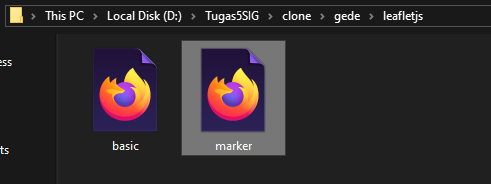
\includegraphics[width=12cm]{figures/Tugas5/1174077/4.png}
		\centering
		\caption{File Marker.html}
	\end{figure}
	\begin{figure}[H]
		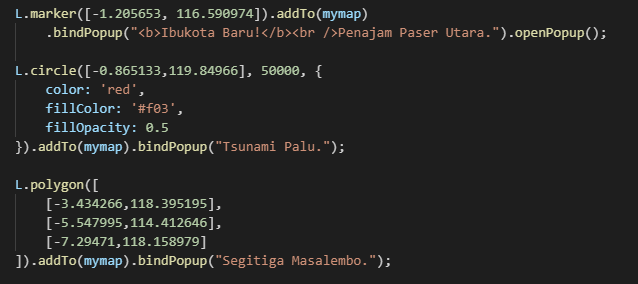
\includegraphics[width=12cm]{figures/Tugas5/1174077/6.png}
		\centering
		\caption{Code tambahan Marker.html}
	\end{figure}
    \item Lalu buka file tersebut dengan browser dan hasilnya akan seperti pada di gambar
    \hfill\break
    \begin{figure}[H]
		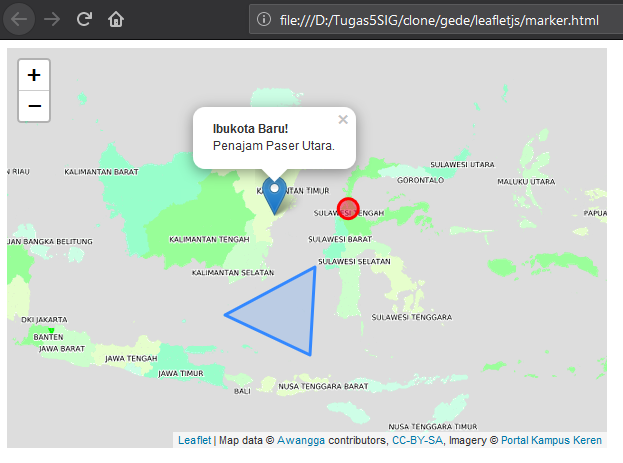
\includegraphics[width=12cm]{figures/Tugas5/1174077/5.png}
		\centering
		\caption{Tampilan Marker.html}
	\end{figure}
\end{enumerate}
\subsection{Link Youtube}
\verb|https://youtu.be/vAlXQWOE_NY|
\section{Muhammad Reza Syachrani (1174084)}
\subsection{Menggunakan LeafletJS dengan MapProxy}
\begin{enumerate}
    \item Kita run terlebih dahulu MapProxy yang telah dibuat kemarin yaitu agm.yaml
    \hfill\break
    \begin{figure}[H]
		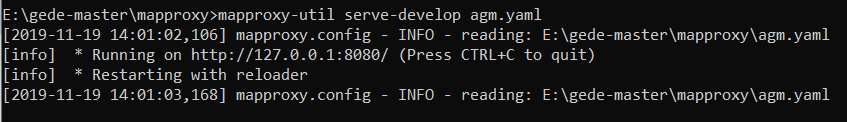
\includegraphics[width=12cm]{figures/Tugas5/1174084/1.png}
		\centering
		\caption{Start server MapProxy}
	\end{figure}
    \item Buka file contoh penggunaan LeafletJS yaitu basic.html di dalam folder leafletjs di dalam folder gede
    \hfill\break
    \begin{figure}[H]
		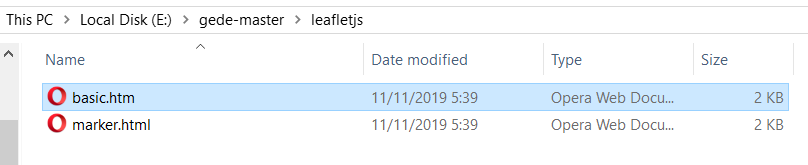
\includegraphics[width=12cm]{figures/Tugas5/1174084/2.png}
		\centering
		\caption{File Basic.html}
	\end{figure}
	\begin{figure}[H]
		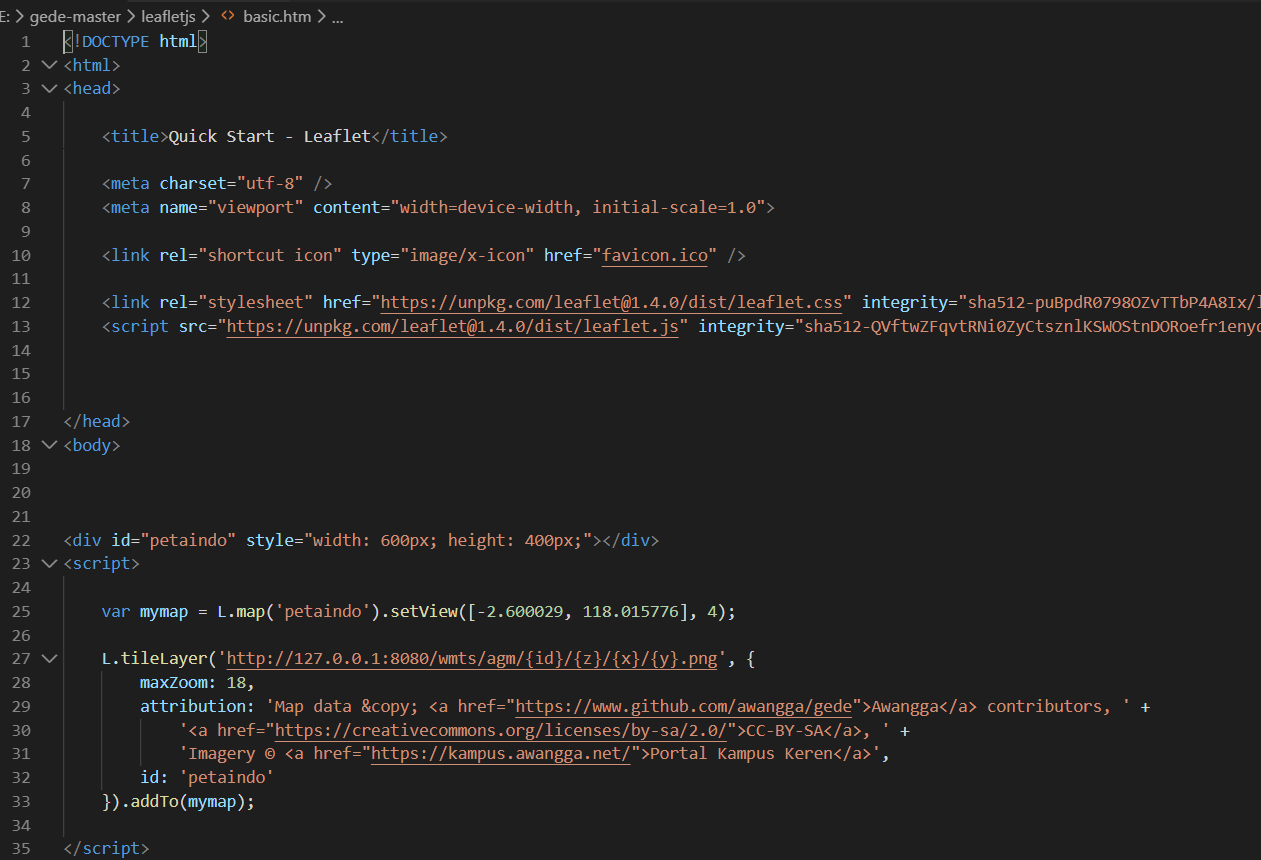
\includegraphics[width=12cm]{figures/Tugas5/1174084/7.png}
		\centering
		\caption{Code Basic.html}
	\end{figure}
    \item Lalu buka file tersebut di browser, maka hasilnya akan seperti ini
    \hfill\break
    \begin{figure}[H]
		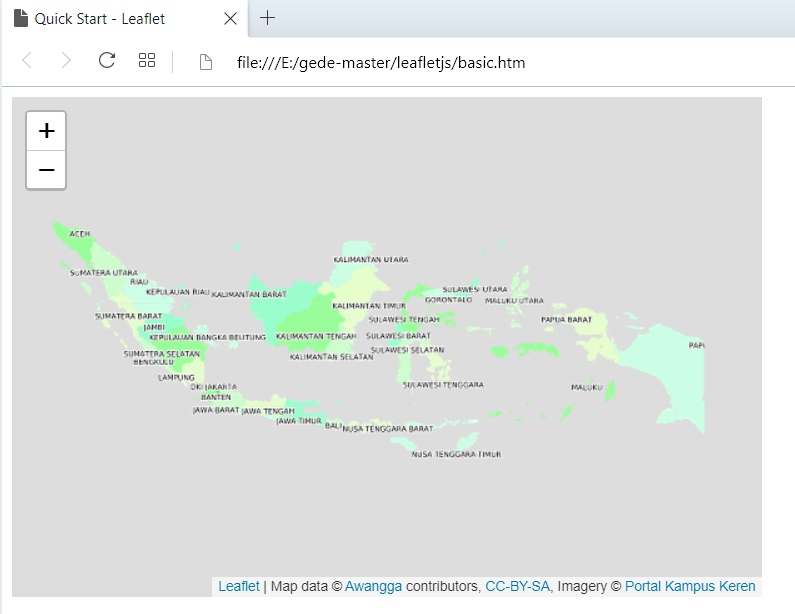
\includegraphics[width=12cm]{figures/Tugas5/1174084/3.png}
		\centering
		\caption{Tampilan Basic.html}
	\end{figure}
    \item Dengan leafletjs kita juga dapat menambahkan marker,circle, ataupun polygon dengan cara menggunakan seperti di gambar, contoh ini diambil dari file contoh kedua yaitu marker.html dari folder gede 
    \hfill\break
    \begin{figure}[H]
		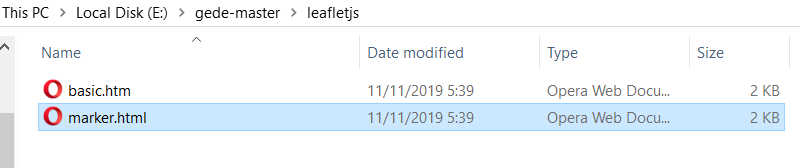
\includegraphics[width=12cm]{figures/Tugas5/1174084/4.png}
		\centering
		\caption{File Marker.html}
	\end{figure}
	\begin{figure}[H]
		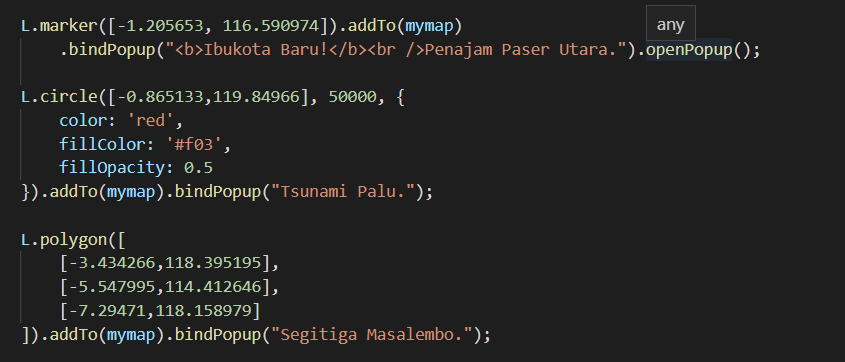
\includegraphics[width=12cm]{figures/Tugas5/1174084/6.png}
		\centering
		\caption{Code tambahan Marker.html}
	\end{figure}
    \item Lalu buka file tersebut dengan browser dan hasilnya akan seperti pada di gambar
    \hfill\break
    \begin{figure}[H]
		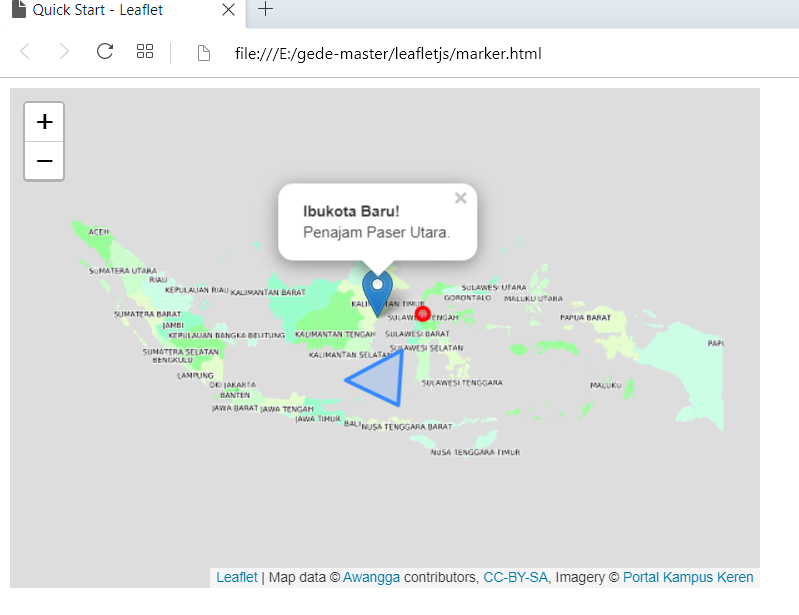
\includegraphics[width=12cm]{figures/Tugas5/1174084/5.png}
		\centering
		\caption{Tampilan Marker.html}
	\end{figure}
\end{enumerate}
\subsection{Link Youtube}
https://youtu.be/obQV7GIeNwQ
\section{Arrial Furqona Gifary (1174070)}
\subsection{LeafletJS dan Mapproxy}
\begin{enumerate}
    \item Langkah pertama yaitu run terlebih dahulu mapproxy nya.
  \hfill\break
  \begin{figure}[H]
  
\includegraphics[width=4cm]{figures/tugas5/1174070/1.png}
  \centering
  \caption{Run Mapproxy}
  \end{figure}
    
   

    \item Setelah itu buka contoh file leafletjs yang ada di dalam folder gede  yang telah kita download sebelumnya .
    
  \hfill\break
  \begin{figure}[H]
  
\includegraphics[width=4cm]{figures/tugas5/1174070/2.png}
  \centering
  \caption{Isi Basic.html}
  \end{figure}
    
    \item Kemudian buka browser, maka hasilnya akan seperti ini
    
  \hfill\break
  \begin{figure}[H]
  \includegraphics[width=4cm]{figures/tugas5/1174070/3.png}
  \centering
  \caption{Hasil dari Basic.html}
  \end{figure}
  
   \item Dengan menggunakan LeafletJS kita dapat menambhakan marker, circle dan polygon yaitu dengan cara seperti gambar dibawah ini, contoh ini diambil dari file marker.html yang berada didalam folder gerede.
    
  \hfill\break
  \begin{figure}[H]
  \includegraphics[width=4cm]{figures/tugas5/1174070/4.png}
  \centering
  \caption{Isi dari marker.html}
  \end{figure}
  
   \item kemudian buka filenya di browser, hasilnya seperti gambar dibawah ini.
  \hfill\break
  \begin{figure}[H]
  
\includegraphics[width=4cm]{figures/tugas5/1174070/5.png}
  \centering
  \caption{Isi dari marker.html}
  \end{figure}

\end{enumerate}

\subsection{Link Youtube MapProxy dan Menjalankannya}
\verb|https://youtu.be/j_zLb519AQ0|
\section{Bakti Qilan Mufid (1174083)}
\subsection{Menggunakan LeafletJS dengan MapProxy}
\begin{enumerate}
    \item Kita run terlebih dahulu MapProxy yang telah dibuat kemarin
    \hfill\break
    \begin{figure}[H]
		\includegraphics[width=12cm]{figures/Tugas5/1174083/pic1.png}
		\centering
		\caption{Gambar 1}
	\end{figure}
    \item Buka file contoh penggunaan LeafletJS yaitu basic.html di dalam folder leafletjs di dalam folder gede yang telah dibuat oleh Bpk.Rolly
    \hfill\break
    \begin{figure}[H]
		\includegraphics[width=12cm]{figures/Tugas5/1174083/pic2.png}
		\centering
		\caption{Gambar 2}
	\end{figure}
    \item Lalu buka file tersebut di browser, maka hasilnya akan seperti ini
    \hfill\break
    \begin{figure}[H]
		\includegraphics[width=12cm]{figures/Tugas5/1174083/pic3.png}
		\centering
		\caption{Gambar 3}
	\end{figure}
    \item Dengan leafletjs kita juga dapat menambahkan marker,circle, ataupun polygon dengan cara menggunakan seperti di gambar, contoh ini diambil
          dari file contoh kedua yaitu marker.html dari folder gede 
    \hfill\break
    \begin{figure}[H]
		\includegraphics[width=12cm]{figures/Tugas5/1174083/pic4.png}
		\centering
		\caption{Gambar 4}
	\end{figure}
	\begin{figure}[H]
		\includegraphics[width=12cm]{figures/Tugas5/1174083/pic5.png}
		\centering
		\caption{Gambar 5}
	\end{figure}
    \item Lalu buka file tersebut dengan browser dan hasilnya akan seperti pada di gambar
    \hfill\break
    \begin{figure}[H]
		\includegraphics[width=12cm]{figures/Tugas5/1174083/pic6.png}
		\centering
		\caption{Gambar 6}
	\end{figure}
\end{enumerate}
\subsection{Link Youtube}
https://youtu.be/7p1VFe86jnQ
\section{Alfadian Owen (1174091)}
\subsection{Menggunakan LeafletJS dengan MapProxy}
\begin{enumerate}
	\item Kita run terlebih dahulu MapProxy yang telah dibuat kemarin
    \hfill\break
    \begin{figure}[H]
		\includegraphics[width=12cm]{figures/Tugas5/1174091/1.png}
		\centering
		\caption{Run Mapproxy}
	\end{figure}
	
	\item Buka file basic.html pada folder leafletjs
    \hfill\break
    \begin{figure}[H]
		\includegraphics[width=12cm]{figures/Tugas5/1174091/2.png}
		\centering
		\caption{Buka basic.html}
	\end{figure}
	
	\item Lalu buka file tersebut di browser, maka hasilnya akan seperti ini
    \hfill\break
    \begin{figure}[H]
		\includegraphics[width=12cm]{figures/Tugas5/1174091/3.png}
		\centering
		\caption{Hasil }
	\end{figure}
	
	\item Dengan leafletjs kita juga dapat menambahkan marker,circle, ataupun polygon dengan cara menggunakan seperti di gambar, contoh ini diambil
          dari file marker.html dari folder gede 
    \hfill\break
	
	\item Buka file marker.html
    \hfill\break
	\begin{figure}[H]
		\includegraphics[width=12cm]{figures/Tugas5/1174091/4.png}
		\centering
		\caption{Hasil marker.html}
	\end{figure}
\end{enumerate}

  
\section{Nurul Izza Hamka (1174062)}
\subsection{Instalasi Map Server}
\begin{enumerate}
    \item Langkah pertama pertama  adalah menginstall MapServer (MS4W)
  \hfill\break
  \begin{figure}[H]
  \includegraphics[width=4cm]{figures/tugas4/1174062/1.png}
  \centering
  \caption{Gambar Link Download MS4W}
  \end{figure}
    
    \item Setelah itu klik file seperti pada gambar dibawah ini untuk di download
    
  \hfill\break
  \begin{figure}[H]
  \includegraphics[width=4cm]{figures/tugas4/1174062/2.png}
  \centering
  \caption{Gambar Untuk Install File exe}
  \end{figure}
  
    \item Setelah itu run MS4W yang telah didownload untuk melanjutkan instalasi
    
  \hfill\break
  \begin{figure}[H]
  \includegraphics[width=4cm]{figures/tugas4/1174062/3.png}
  \centering
  \caption{Gambar Proses Instalasi Ms4w}
  \end{figure}
  
\end{enumerate}

\subsection{Konfigurasi Map Server}
Langkah selanjutnya setelah proses intalasi, maka kita akan melakukan konfigurasi
\begin{enumerate}
  \item Buka folder ms4w. Masuk ke folder apache, kemudian masuk ke folder conf dan pilih file httpd.conf
\hfill\break
  \begin{figure}[H]
  \includegraphics[width=4cm]{figures/tugas4/1174062/5.png}
  \centering
  \caption{Gambar Untuk File http.conf}
  \end{figure}
  
  \item Buka file httpd.conf dan ubah listen port nya menjadi port 80.
  
\hfill\break
  \begin{figure}[H]
  \includegraphics[width=4cm]{figures/tugas4/1174062/6.png}
  \centering
  \caption{Gambar Listen port 80}
  \end{figure}
  
  \item Kemudian klik windows + r dan ketikan perintah services.msc
    
\hfill\break
  \begin{figure}[H]
  \includegraphics[width=4cm]{figures/tugas4/1174062/7.png}
  \centering
  \caption{Gambar Untuk Mengakses Halaman Service}
  \end{figure}
  
  \item Kemudian Pilih MS4W untuk Web Server, kemudian Klik OK
 \hfill\break
  \begin{figure}[H]
  \includegraphics[width=4cm]{figures/tugas4/1174062/4.png}
  \centering
  \caption{Gambar Untuk Mengakses Halaman Service}
  \end{figure}
  
\subsection{Pengujian}
\begin{enumerate}
	\item Setelah dilakukan Konfigurasi maka kita akan melakukan pengujian, ada dua file yang dibutuhkan yaitu .map dan .ymal
  \item Pertama masuk ke web dengan Link https://github.com/awangga/gede/

 \hfill\break
  \begin{figure}[H]
  \includegraphics[width=4cm]{figures/tugas4/1174062/8.png}
  \centering
  \caption{Link Github}
  \end{figure}


  \item Kemudian file Clone atau Download, selanjutnya Download ZIP
  
    \hfill\break
    \begin{figure}[H]
  \includegraphics[width=4cm]{figures/tugas4/1174062/9.png}
  \centering
  \caption{Gambar Untuk Download File}
  \end{figure}

  \item Kemudian buka file agm.ymal  pada file yang telah didownload tadi untuk meyesuaikan file directori kita
    
    \hfill\break
    \begin{figure}[H]
  \includegraphics[width=4cm]{figures/tugas4/1174062/10.png}
  \centering
  \caption{Gambar di File aqm.ymal}
  \end{figure}
  
   \item Selajutnya buka app QGIS
  
 \hfill\break
    \begin{figure}[H]
  \includegraphics[width=4cm]{figures/tugas4/1174062/11.png}
  \centering
  \caption{Gambar Untuk Aplikasi QGIS}
  \end{figure}
  
  \item Selajutnya buka File 00.shp 
  
 \hfill\break
    \begin{figure}[H]
  \includegraphics[width=4cm]{figures/tugas4/1174062/12.png}
  \centering
  \caption{Gambar Hasil 00.shp}
  \end{figure}

 \item Selajutnya jalankan file bts negara.shp
   
 \hfill\break
    \begin{figure}[H]
  \includegraphics[width=4cm]{figures/tugas4/1174062/13.png}
  \centering
  \caption{Gambar Hasil bts negara.shp}
  \end{figure}
 
\end{enumerate}
\subsection{Link Youtube Instalasi MapServer}
{https://www.youtube.com/watch?v=BkFsJXB1vJ8}

\subsection{Instalasi MapProxy}
\begin{enumerate}
  \item Pertama buka Command Prompt
  \item Lalu ketikkan pip install MapProxy
  \hfill\break
  \begin{figure}[H]
  \includegraphics[width=4cm]{figures/tugas4/1174062/14.png}
  \centering
  \caption{Instalasi MapProxy}
  \end{figure}

\end{enumerate}

\subsection{Link Youtube MapProxy dan Menjalankannya}
https://www.youtube.com/watch?v=E8SSxJZm9k8
\section{ainulfiliani (1174073)}
\subsection{LeafletJS dan MapProxy}
\begin{enumerate}
    \item Jalankan terlebih dahulu mapproxy pada folder gede dengan menggunakan setingan agm.yaml
        \hfill\break
        \begin{figure}[H]
        \includegraphics[width=4cm]{figures/tugas5/1174073/1.jpg}
        \centering
        \caption{Menjalankan Mapproxy}
        \end{figure}
        
        
    \item Setelah itu buka contoh file leafletjs yang ada di dalam folder gede  yang telah kita download sebelumnya .
    
  \hfill\break
  \begin{figure}[H]
  \includegraphics[width=4cm]{figures/tugas5/1174073/2.jpg}
  \centering
  \caption{Isi Basic.html}
  \end{figure}
  
    \item Setelah itu buka file basic.html pada folder leafletjs yang ada di dalam folder gede menggunakan browser
        \hfill\break
        \begin{figure}[H]
        
        
        \includegraphics[width=4cm]{figures/tugas5/1174073/3.jpg}
        \centering
        \caption{Hasil dari file basic.htm}
        \end{figure}
   \item Dengan menggunakan LeafletJS kita dapat menambahkan marker, circle dan polygon yaitu dengan cara seperti gambar dibawah ini yang ada pada file marker.html pada folder gede/leafletjs
        \hfill\break
        \begin{figure}[H]
        \includegraphics[width=4cm]{figures/tugas5/1174073/4.jpg}
        \centering
        \caption{Contoh menambahkan marker, circle dan polygon}
        \end{figure}
   \item Apabila file tersebut dibuka di browser maka akan muncul seperti ini
        \hfill\break
        \begin{figure}[H]
        \includegraphics[width=4cm]{figures/tugas5/1174073/5.jpg}
        \centering
        \caption{Hasil dari file marker.html}
        \end{figure}
\end{enumerate}
\subsection{Link Youtube LeafletJS dan MapProxy}
https://youtu.be/iAg1eAVkTqY


\section{Aulyardha Anindita | 1174054}
\subsection{LeafletJS dan Mapproxy}
\begin{enumerate}
\item Pertama,run terlebih dahulu map proxy nya. Untuk ngerun nya sama seperti pada tugas sebelumnya. Untuk lebih jelasnya dapat dilihat pada gambar berikut:
\hfill\break
\begin{figure}[H]
\includegraphics[width=4cm]{figures/tugas5/1174054/1.png}
\centering
\caption{Run Mapproxy}
\end{figure}
    
\item Selanjutnya, buka contoh file leafletjs yang sudah kita download sebelumnya yang berada didalam folder gede. 
\hfill\break
\begin{figure}[H]
\includegraphics[width=4cm]{figures/tugas5/1174054/2.png}
\centering
\caption{Isi Basic.htm}
\end{figure}
    
\item Kemudian buka browser, dan jika berhasil maka hasilnya akan seperti pada gambar berikut :
\hfill\break
\begin{figure}[H]
\includegraphics[width=4cm]{figures/tugas5/1174054/3.png}
\centering
\caption{Hasil dari Basic.html}
\end{figure}
  
\item Dengan menggunakan LeafletJS kita dapat menambahkan marker, circle dan polygon yaitu dengan cara seperti gambar dibawah ini, contoh ini diambil dari file marker.html yang berada didalam folder gede.
\hfill\break
\begin{figure}[H]
\includegraphics[width=4cm]{figures/tugas5/1174054/4.png}
\centering
\caption{Isi dari marker.html}
\end{figure}
  
\item kemudian buka filenya di browser, hasilnya seperti gambar dibawah ini.
\hfill\break
\begin{figure}[H]
\includegraphics[width=4cm]{figures/tugas5/1174054/5.png}
\centering
\caption{Isi dari marker.html}
\end{figure}

\end{enumerate}

\subsection{Link Youtube LeafletsJS}
https://youtu.be/pBx5bSk2lmI
\section{Difa Al Fansha (1174076)}
\subsection{Menggunakan LeafletJS dengan MapProxy}
\begin{enumerate}
	\item Kita run terlebih dahulu MapProxy yang telah dibuat kemarin
    \hfill\break
    \begin{figure}[H]
		\includegraphics[width=12cm]{figures/Tugas5/1174076/1.png}
		\centering
		\caption{Run Mapproxy}
	\end{figure}
	
	\item Buka file basic.html pada folder leafletjs
    \hfill\break
    \begin{figure}[H]
		\includegraphics[width=12cm]{figures/Tugas5/1174076/2.png}
		\centering
		\caption{Open basic.html}
	\end{figure}
	
	\item Lalu buka file tersebut di browser, maka hasilnya akan seperti ini
    \hfill\break
    \begin{figure}[H]
		\includegraphics[width=12cm]{figures/Tugas5/1174076/3.png}
		\centering
		\caption{Hasil basic.html}
	\end{figure}
	
	\item Dengan leafletjs kita juga dapat menambahkan marker,circle, ataupun polygon dengan cara menggunakan seperti di gambar, contoh ini diambil
          dari file contoh kedua yaitu marker.html dari folder gede 
    \hfill\break
	
	\item Buka file marker.html
    \hfill\break
	\begin{figure}[H]
		\includegraphics[width=12cm]{figures/Tugas5/1174076/4.png}
		\centering
		\caption{Hasil marker.html}
	\end{figure}
\end{enumerate}

\subsection{Link}
\url{https://youtu.be/xWDgij_GD_E}
  
\input{chapters/tugas1/1174074}
\section{Muhammad Abdul Gani Wijaya (1174071)}
\subsection{Menggunakan LeafletJS dengan MapProxy}
\begin{enumerate}
	\item Pertama-tama jalankan mapproxy yang telah dibuat pada praktikum sebelumnya
    \hfill\break
    \begin{figure}[H]
		\includegraphics[width=12cm]{figures/Tugas5/1174071/1.png}
		\centering
		\caption{Run Mapproxy}
	\end{figure}
	
	\item Buka folder leafjs yang ada di folder gede, lalu buka file basic.html
    \hfill\break
    \begin{figure}[H]
		\includegraphics[width=12cm]{figures/Tugas5/1174071/2.png}
		\centering
		\caption{File basic.html}
	\end{figure}
	
	\item Buka file basic.html di browser, maka hasilnya akan seperti ini
    \hfill\break
    \begin{figure}[H]
		\includegraphics[width=12cm]{figures/Tugas5/1174071/3.png}
		\centering
		\caption{Hasil basic.html}
	\end{figure}
	
	\item Dengan leafletjs kita juga dapat menambahkan marker,circle, ataupun polygon dengan cara menggunakan L.marker, L.circle,  dan L.polygon. Contohnya file marker.html
    \hfill\break
	
	\item Buka file marker.html di text editor
    \hfill\break
	\begin{figure}[H]
		\includegraphics[width=12cm]{figures/Tugas5/1174071/4.png}
		\centering
		\caption{Kode untuk menggunakan marker, circle, dan polygon}
	\end{figure}

	\item Lalu buka file marker.html di web browser, dan seperti ini hasilnya
    \hfill\break
	\begin{figure}[H]
		\includegraphics[width=12cm]{figures/Tugas5/1174071/5.png}
		\centering
		\caption{Hasil marker.html}
	\end{figure}
\end{enumerate}

\subsection{Link}
\url{https://youtu.be/iucxbB81h1A}
  
\section{Handi Hermawan (1174080)}
\subsection{Menggunakan LeafletJS dengan MapProxy}
\begin{enumerate}
    \item Pertama jalankan MapProxy yang telah dibuat sebelumnya yaitu file agm.yaml
    \hfill\break
    \begin{figure}[H]
		\includegraphics[width=12cm]{figures/Tugas5/1174080/1.png}
		\centering
		\caption{Start server MapProxy}
	\end{figure}
    \item Kedua buka file contoh penggunaan LeafletJS yaitu basic.html di dalam folder leafletjs di folder gede
    \hfill\break
    \begin{figure}[H]
		\includegraphics[width=12cm]{figures/Tugas5/1174080/2.png}
		\centering
		\caption{File Basic.html}
	\end{figure}
	\begin{figure}[H]
		\includegraphics[width=12cm]{figures/Tugas5/1174080/3.png}
		\centering
		\caption{Code Basic.html}
	\end{figure}
    \item Ketiga buka file tersebut di browser, maka hasilnya akan seperti ini
    \hfill\break
    \begin{figure}[H]
		\includegraphics[width=12cm]{figures/Tugas5/1174080/4.png}
		\centering
		\caption{Tampilan Basic.html}
	\end{figure}
    \item Di leafletjs kita juga dapat menambahkan marker,circle, ataupun polygon dengan cara menggunakan seperti di gambar, contoh ini diambil dari file contoh kedua yaitu marker.html dari folder gede 
    \hfill\break
    \begin{figure}[H]
		\includegraphics[width=12cm]{figures/Tugas5/1174080/5.png}
		\centering
		\caption{File Marker.html}
	\end{figure}
	\begin{figure}[H]
		\includegraphics[width=12cm]{figures/Tugas5/1174080/6.png}
		\centering
		\caption{Code tambahan Marker.html}
	\end{figure}
    \item Terakhir buka file tersebut dengan browser dan hasilnya akan seperti pada di gambar
    \hfill\break
    \begin{figure}[H]
		\includegraphics[width=12cm]{figures/Tugas5/1174080/7.png}
		\centering
		\caption{Tampilan Marker.html}
	\end{figure}
\end{enumerate}
\subsection{Link Youtube}
https://youtu.be/zXuClvJ5OYE
\input{chapters/tugas1/1174053}
\chapter{Tugas Kedua}
\section{D. Irga B. Naufal Fakrhi (1174066)}
\subsection{LeafletJS dan MapProxy}
\begin{enumerate}
    \item Jalankan terlebih dahulu mapproxy pada folder gede dengan menggunakan setingan agm.yaml
        \hfill\break
        \begin{figure}[H]
        \includegraphics[width=4cm]{figures/tugas5/1174066/1.jpg}
        \centering
        \caption{Menjalankan Mapproxy}
        \end{figure}
    \item Setelah itu buka file basic.html pada folder leafletjs yang ada di dalam folder gede menggunakan browser
        \hfill\break
        \begin{figure}[H]
        \includegraphics[width=4cm]{figures/tugas5/1174066/3.jpg}
        \centering
        \caption{Hasil dari file basic.htm}
        \end{figure}
   \item Dengan menggunakan LeafletJS kita dapat menambahkan marker, circle dan polygon yaitu dengan cara seperti gambar dibawah ini yang ada pada file marker.html pada folder gede/leafletjs
        \hfill\break
        \begin{figure}[H]
        \includegraphics[width=4cm]{figures/tugas5/1174066/4.jpg}
        \centering
        \caption{Contoh menambahkan marker, circle dan polygon}
        \end{figure}
   \item Apabila file tersebut dibuka di browser maka akan muncul seperti ini
        \hfill\break
        \begin{figure}[H]
        \includegraphics[width=4cm]{figures/tugas5/1174066/5.jpg}
        \centering
        \caption{Hasil dari file marker.html}
        \end{figure}
\end{enumerate}
\subsection{Link Youtube LeafletJS dan MapProxy}
https://youtu.be/cW\_TD69y62U

\section{Chandra Kirana Poetra (1174079)}
\subsection{Menggunakan LeafletJS dengan MapProxy}
\begin{enumerate}
    \item Jalankan dulu mapproxy yang kemarin telah dibuat di gede-master
    \hfill\break
    \begin{figure}[H]
		\includegraphics[width=12cm]{figures/Tugas5/1174079/1.png}
		\centering
		\caption{Gambar 1}
	\end{figure}
    \item Buka file basic.html di folder LeafletJS di dalam folder gede
    \hfill\break
    \begin{figure}[H]
		\includegraphics[width=12cm]{figures/Tugas5/1174079/2.png}
		\centering
		\caption{Gambar 2}
	\end{figure}
    \item Berikut adalah hasil dari file basic.html
    \hfill\break
    \begin{figure}[H]
		\includegraphics[width=12cm]{figures/Tugas5/1174079/3.png}
		\centering
		\caption{Gambar 3}
	\end{figure}
    \item Di leafletjs kita juga bisa menambahkan penanda atau marker,circle, ataupun polygon sebagai penanda dengan cara seperti di gambar
    \hfill\break
    \begin{figure}[H]
		\includegraphics[width=12cm]{figures/Tugas5/1174079/2.png}
		\centering
		\caption{Gambar 4}
	\end{figure}
	\begin{figure}[H]
		\includegraphics[width=12cm]{figures/Tugas5/1174079/4.png}
		\centering
		\caption{Gambar 5}
	\end{figure}
    \item Lalu coba buka di browser
    \hfill\break
    \begin{figure}[H]
		\includegraphics[width=12cm]{figures/Tugas5/1174079/5.png}
		\centering
		\caption{Gambar 6}
	\end{figure}
\end{enumerate}
\subsection{Link Youtube}
https://youtu.be/0PGjQqv-Dec
\section{Tia Nur Candida (1174086)}
\subsection{Menggunakan LeafletJS dengan MapProxy}
\begin{enumerate}
    \item Run terlebih dahulu Mapproxy
    \hfill\break
    \begin{figure}[H]
		\includegraphics[width=12cm]{figures/Tugas5/1174086/1.png}
		\centering
		\caption{Gambar 1}
	\end{figure}
    \item Buka file basic.html di dalam folder leafletjs di dalam folder gede
    \hfill\break
    \begin{figure}[H]
		\includegraphics[width=12cm]{figures/Tugas5/1174086/3.png}
		\centering
		\caption{Gambar 2}
	\end{figure}
    \item Lalu buka file tersebut di browser, maka hasilnya akan seperti berikut
    \hfill\break
    \begin{figure}[H]
		\includegraphics[width=12cm]{figures/Tugas5/1174086/4.png}
		\centering
		\caption{Gambar 3}
	\end{figure}
    \item Pada leafletjs dapat menambahkan marker,circle, ataupun polygon 
    \hfill\break
    \begin{figure}[H]
		\includegraphics[width=12cm]{figures/Tugas5/1174086/5.png}
		\centering
		\caption{Gambar 4}
	\end{figure}
    \item Lalu buka file tersebut dengan browser dan hasilnya akan seperti berikut
    \hfill\break
    \begin{figure}[H]
		\includegraphics[width=12cm]{figures/Tugas5/1174086/6.png}
		\centering
		\caption{Gambar 5}
	\end{figure}
\end{enumerate}
\subsection{Link Youtube}
https://youtu.be/Qqu4UE9od9w
\section{Muhammad Abdul Gani Wijaya (1174071)}
\subsection{Menggunakan LeafletJS dengan MapProxy}
\begin{enumerate}
	\item Pertama-tama jalankan mapproxy yang telah dibuat pada praktikum sebelumnya
    \hfill\break
    \begin{figure}[H]
		\includegraphics[width=12cm]{figures/Tugas5/1174071/1.png}
		\centering
		\caption{Run Mapproxy}
	\end{figure}
	
	\item Buka folder leafjs yang ada di folder gede, lalu buka file basic.html
    \hfill\break
    \begin{figure}[H]
		\includegraphics[width=12cm]{figures/Tugas5/1174071/2.png}
		\centering
		\caption{File basic.html}
	\end{figure}
	
	\item Buka file basic.html di browser, maka hasilnya akan seperti ini
    \hfill\break
    \begin{figure}[H]
		\includegraphics[width=12cm]{figures/Tugas5/1174071/3.png}
		\centering
		\caption{Hasil basic.html}
	\end{figure}
	
	\item Dengan leafletjs kita juga dapat menambahkan marker,circle, ataupun polygon dengan cara menggunakan L.marker, L.circle,  dan L.polygon. Contohnya file marker.html
    \hfill\break
	
	\item Buka file marker.html di text editor
    \hfill\break
	\begin{figure}[H]
		\includegraphics[width=12cm]{figures/Tugas5/1174071/4.png}
		\centering
		\caption{Kode untuk menggunakan marker, circle, dan polygon}
	\end{figure}

	\item Lalu buka file marker.html di web browser, dan seperti ini hasilnya
    \hfill\break
	\begin{figure}[H]
		\includegraphics[width=12cm]{figures/Tugas5/1174071/5.png}
		\centering
		\caption{Hasil marker.html}
	\end{figure}
\end{enumerate}

\subsection{Link}
\url{https://youtu.be/iucxbB81h1A}
  
\section{Muhammad Reza Syachrani (1174084)}
\subsection{Menggunakan LeafletJS dengan MapProxy}
\begin{enumerate}
    \item Kita run terlebih dahulu MapProxy yang telah dibuat kemarin yaitu agm.yaml
    \hfill\break
    \begin{figure}[H]
		\includegraphics[width=12cm]{figures/Tugas5/1174084/1.png}
		\centering
		\caption{Start server MapProxy}
	\end{figure}
    \item Buka file contoh penggunaan LeafletJS yaitu basic.html di dalam folder leafletjs di dalam folder gede
    \hfill\break
    \begin{figure}[H]
		\includegraphics[width=12cm]{figures/Tugas5/1174084/2.png}
		\centering
		\caption{File Basic.html}
	\end{figure}
	\begin{figure}[H]
		\includegraphics[width=12cm]{figures/Tugas5/1174084/7.png}
		\centering
		\caption{Code Basic.html}
	\end{figure}
    \item Lalu buka file tersebut di browser, maka hasilnya akan seperti ini
    \hfill\break
    \begin{figure}[H]
		\includegraphics[width=12cm]{figures/Tugas5/1174084/3.png}
		\centering
		\caption{Tampilan Basic.html}
	\end{figure}
    \item Dengan leafletjs kita juga dapat menambahkan marker,circle, ataupun polygon dengan cara menggunakan seperti di gambar, contoh ini diambil dari file contoh kedua yaitu marker.html dari folder gede 
    \hfill\break
    \begin{figure}[H]
		\includegraphics[width=12cm]{figures/Tugas5/1174084/4.png}
		\centering
		\caption{File Marker.html}
	\end{figure}
	\begin{figure}[H]
		\includegraphics[width=12cm]{figures/Tugas5/1174084/6.png}
		\centering
		\caption{Code tambahan Marker.html}
	\end{figure}
    \item Lalu buka file tersebut dengan browser dan hasilnya akan seperti pada di gambar
    \hfill\break
    \begin{figure}[H]
		\includegraphics[width=12cm]{figures/Tugas5/1174084/5.png}
		\centering
		\caption{Tampilan Marker.html}
	\end{figure}
\end{enumerate}
\subsection{Link Youtube}
https://youtu.be/obQV7GIeNwQ
\section{Fanny Shafira Damayanti (1174069)}
\subsection{LeafletJS dan Mapproxy}
\begin{enumerate}
    \item Langkah pertama yaitu run terlebih dahulu mapproxy nya.
  \hfill\break
  \begin{figure}[H]
  \includegraphics[width=4cm]{figures/tugas5/1174069/1.png}
  \centering
  \caption{Run Mapproxy}
  \end{figure}
    
   

    \item Setelah itu buka contoh file leafletjs yang ada di dalam folder gede  yang telah kita download sebelumnya .
    
  \hfill\break
  \begin{figure}[H]
  \includegraphics[width=4cm]{figures/tugas5/1174069/2.png}
  \centering
  \caption{Isi Basic.html}
  \end{figure}
    
    \item Kemudian buka browser, maka hasilnya akan seperti ini
    
  \hfill\break
  \begin{figure}[H]
  \includegraphics[width=4cm]{figures/tugas5/1174069/3.png}
  \centering
  \caption{Hasil dari Basic.html}
  \end{figure}
  
   \item Dengan menggunakan LeafletJS kita dapat menambhakan marker, circle dan polygon yaitu dengan cara seperti gambar dibawah ini, contoh ini diambil dari file marker.html yang berada didalam folder gerede.
    
  \hfill\break
  \begin{figure}[H]
  \includegraphics[width=4cm]{figures/tugas5/1174069/4.png}
  \centering
  \caption{Isi dari marker.html}
  \end{figure}
  
   \item kemudian buka filenya di browser, hasilnya seperti gambar dibawah ini.
  \hfill\break
  \begin{figure}[H]
  \includegraphics[width=4cm]{figures/tugas5/1174069/5.png}
  \centering
  \caption{Isi dari marker.html}
  \end{figure}

\end{enumerate}

\subsection{Link Youtube MapProxy dan Menjalankannya}
\verb|https://youtu.be/j_zLb519AQ0|
\section{Bakti Qilan Mufid (1174083)}
\subsection{Menggunakan LeafletJS dengan MapProxy}
\begin{enumerate}
    \item Kita run terlebih dahulu MapProxy yang telah dibuat kemarin
    \hfill\break
    \begin{figure}[H]
		\includegraphics[width=12cm]{figures/Tugas5/1174083/pic1.png}
		\centering
		\caption{Gambar 1}
	\end{figure}
    \item Buka file contoh penggunaan LeafletJS yaitu basic.html di dalam folder leafletjs di dalam folder gede yang telah dibuat oleh Bpk.Rolly
    \hfill\break
    \begin{figure}[H]
		\includegraphics[width=12cm]{figures/Tugas5/1174083/pic2.png}
		\centering
		\caption{Gambar 2}
	\end{figure}
    \item Lalu buka file tersebut di browser, maka hasilnya akan seperti ini
    \hfill\break
    \begin{figure}[H]
		\includegraphics[width=12cm]{figures/Tugas5/1174083/pic3.png}
		\centering
		\caption{Gambar 3}
	\end{figure}
    \item Dengan leafletjs kita juga dapat menambahkan marker,circle, ataupun polygon dengan cara menggunakan seperti di gambar, contoh ini diambil
          dari file contoh kedua yaitu marker.html dari folder gede 
    \hfill\break
    \begin{figure}[H]
		\includegraphics[width=12cm]{figures/Tugas5/1174083/pic4.png}
		\centering
		\caption{Gambar 4}
	\end{figure}
	\begin{figure}[H]
		\includegraphics[width=12cm]{figures/Tugas5/1174083/pic5.png}
		\centering
		\caption{Gambar 5}
	\end{figure}
    \item Lalu buka file tersebut dengan browser dan hasilnya akan seperti pada di gambar
    \hfill\break
    \begin{figure}[H]
		\includegraphics[width=12cm]{figures/Tugas5/1174083/pic6.png}
		\centering
		\caption{Gambar 6}
	\end{figure}
\end{enumerate}
\subsection{Link Youtube}
https://youtu.be/7p1VFe86jnQ
\section{Kaka Kamaludin (1174067)}
\subsection{LeafletJS dan MapProxy}
\begin{enumerate}
    \item Jalankan terlebih dahulu mapproxy pada folder gede dengan menggunakan setingan agm.yaml
        \hfill\break
        \begin{figure}[H]
        \includegraphics[width=4cm]{figures/tugas5/1174067/1.png}
        \centering
        \caption{Menjalankan Mapproxy}
        \end{figure}
    \item Setelah itu buka file basic.html pada folder leafletjs yang ada di dalam folder gede menggunakan browser
        \hfill\break
        \begin{figure}[H]
        \includegraphics[width=4cm]{figures/tugas5/1174067/3.png}
        \centering
        \caption{Hasil dari file basic.htm}
        \end{figure}
   \item Dengan menggunakan LeafletJS kita dapat menambahkan marker, circle dan polygon yaitu dengan cara seperti gambar dibawah ini yang ada pada file marker.html pada folder gede/leafletjs
        \hfill\break
        \begin{figure}[H]
        \includegraphics[width=4cm]{figures/tugas5/1174067/4.png}
        \centering
        \caption{Contoh menambahkan marker, circle dan polygon}
        \end{figure}
   \item Apabila file tersebut dibuka di browser maka akan muncul seperti ini
        \hfill\break
        \begin{figure}[H]
        \includegraphics[width=4cm]{figures/tugas5/1174067/5.png}
        \centering
        \caption{Hasil dari file marker.html}
        \end{figure}
\end{enumerate}
\subsection{Link Youtube LeafletJS dan MapProxy}
https://youtu.be/xJqh\_aY9Exk

\section{Handi Hermawan (1174080)}
\subsection{Menggunakan LeafletJS dengan MapProxy}
\begin{enumerate}
    \item Pertama jalankan MapProxy yang telah dibuat sebelumnya yaitu file agm.yaml
    \hfill\break
    \begin{figure}[H]
		\includegraphics[width=12cm]{figures/Tugas5/1174080/1.png}
		\centering
		\caption{Start server MapProxy}
	\end{figure}
    \item Kedua buka file contoh penggunaan LeafletJS yaitu basic.html di dalam folder leafletjs di folder gede
    \hfill\break
    \begin{figure}[H]
		\includegraphics[width=12cm]{figures/Tugas5/1174080/2.png}
		\centering
		\caption{File Basic.html}
	\end{figure}
	\begin{figure}[H]
		\includegraphics[width=12cm]{figures/Tugas5/1174080/3.png}
		\centering
		\caption{Code Basic.html}
	\end{figure}
    \item Ketiga buka file tersebut di browser, maka hasilnya akan seperti ini
    \hfill\break
    \begin{figure}[H]
		\includegraphics[width=12cm]{figures/Tugas5/1174080/4.png}
		\centering
		\caption{Tampilan Basic.html}
	\end{figure}
    \item Di leafletjs kita juga dapat menambahkan marker,circle, ataupun polygon dengan cara menggunakan seperti di gambar, contoh ini diambil dari file contoh kedua yaitu marker.html dari folder gede 
    \hfill\break
    \begin{figure}[H]
		\includegraphics[width=12cm]{figures/Tugas5/1174080/5.png}
		\centering
		\caption{File Marker.html}
	\end{figure}
	\begin{figure}[H]
		\includegraphics[width=12cm]{figures/Tugas5/1174080/6.png}
		\centering
		\caption{Code tambahan Marker.html}
	\end{figure}
    \item Terakhir buka file tersebut dengan browser dan hasilnya akan seperti pada di gambar
    \hfill\break
    \begin{figure}[H]
		\includegraphics[width=12cm]{figures/Tugas5/1174080/7.png}
		\centering
		\caption{Tampilan Marker.html}
	\end{figure}
\end{enumerate}
\subsection{Link Youtube}
https://youtu.be/zXuClvJ5OYE
\input{chapters/tugas2/1174089}
\section{Nurul Izza Hamka (1174062)}
\subsection{Instalasi Map Server}
\begin{enumerate}
    \item Langkah pertama pertama  adalah menginstall MapServer (MS4W)
  \hfill\break
  \begin{figure}[H]
  \includegraphics[width=4cm]{figures/tugas4/1174062/1.png}
  \centering
  \caption{Gambar Link Download MS4W}
  \end{figure}
    
    \item Setelah itu klik file seperti pada gambar dibawah ini untuk di download
    
  \hfill\break
  \begin{figure}[H]
  \includegraphics[width=4cm]{figures/tugas4/1174062/2.png}
  \centering
  \caption{Gambar Untuk Install File exe}
  \end{figure}
  
    \item Setelah itu run MS4W yang telah didownload untuk melanjutkan instalasi
    
  \hfill\break
  \begin{figure}[H]
  \includegraphics[width=4cm]{figures/tugas4/1174062/3.png}
  \centering
  \caption{Gambar Proses Instalasi Ms4w}
  \end{figure}
  
\end{enumerate}

\subsection{Konfigurasi Map Server}
Langkah selanjutnya setelah proses intalasi, maka kita akan melakukan konfigurasi
\begin{enumerate}
  \item Buka folder ms4w. Masuk ke folder apache, kemudian masuk ke folder conf dan pilih file httpd.conf
\hfill\break
  \begin{figure}[H]
  \includegraphics[width=4cm]{figures/tugas4/1174062/5.png}
  \centering
  \caption{Gambar Untuk File http.conf}
  \end{figure}
  
  \item Buka file httpd.conf dan ubah listen port nya menjadi port 80.
  
\hfill\break
  \begin{figure}[H]
  \includegraphics[width=4cm]{figures/tugas4/1174062/6.png}
  \centering
  \caption{Gambar Listen port 80}
  \end{figure}
  
  \item Kemudian klik windows + r dan ketikan perintah services.msc
    
\hfill\break
  \begin{figure}[H]
  \includegraphics[width=4cm]{figures/tugas4/1174062/7.png}
  \centering
  \caption{Gambar Untuk Mengakses Halaman Service}
  \end{figure}
  
  \item Kemudian Pilih MS4W untuk Web Server, kemudian Klik OK
 \hfill\break
  \begin{figure}[H]
  \includegraphics[width=4cm]{figures/tugas4/1174062/4.png}
  \centering
  \caption{Gambar Untuk Mengakses Halaman Service}
  \end{figure}
  
\subsection{Pengujian}
\begin{enumerate}
	\item Setelah dilakukan Konfigurasi maka kita akan melakukan pengujian, ada dua file yang dibutuhkan yaitu .map dan .ymal
  \item Pertama masuk ke web dengan Link https://github.com/awangga/gede/

 \hfill\break
  \begin{figure}[H]
  \includegraphics[width=4cm]{figures/tugas4/1174062/8.png}
  \centering
  \caption{Link Github}
  \end{figure}


  \item Kemudian file Clone atau Download, selanjutnya Download ZIP
  
    \hfill\break
    \begin{figure}[H]
  \includegraphics[width=4cm]{figures/tugas4/1174062/9.png}
  \centering
  \caption{Gambar Untuk Download File}
  \end{figure}

  \item Kemudian buka file agm.ymal  pada file yang telah didownload tadi untuk meyesuaikan file directori kita
    
    \hfill\break
    \begin{figure}[H]
  \includegraphics[width=4cm]{figures/tugas4/1174062/10.png}
  \centering
  \caption{Gambar di File aqm.ymal}
  \end{figure}
  
   \item Selajutnya buka app QGIS
  
 \hfill\break
    \begin{figure}[H]
  \includegraphics[width=4cm]{figures/tugas4/1174062/11.png}
  \centering
  \caption{Gambar Untuk Aplikasi QGIS}
  \end{figure}
  
  \item Selajutnya buka File 00.shp 
  
 \hfill\break
    \begin{figure}[H]
  \includegraphics[width=4cm]{figures/tugas4/1174062/12.png}
  \centering
  \caption{Gambar Hasil 00.shp}
  \end{figure}

 \item Selajutnya jalankan file bts negara.shp
   
 \hfill\break
    \begin{figure}[H]
  \includegraphics[width=4cm]{figures/tugas4/1174062/13.png}
  \centering
  \caption{Gambar Hasil bts negara.shp}
  \end{figure}
 
\end{enumerate}
\subsection{Link Youtube Instalasi MapServer}
{https://www.youtube.com/watch?v=BkFsJXB1vJ8}

\subsection{Instalasi MapProxy}
\begin{enumerate}
  \item Pertama buka Command Prompt
  \item Lalu ketikkan pip install MapProxy
  \hfill\break
  \begin{figure}[H]
  \includegraphics[width=4cm]{figures/tugas4/1174062/14.png}
  \centering
  \caption{Instalasi MapProxy}
  \end{figure}

\end{enumerate}

\subsection{Link Youtube MapProxy dan Menjalankannya}
https://www.youtube.com/watch?v=E8SSxJZm9k8
\section{Alfadian Owen (1174091)}
\subsection{Menggunakan LeafletJS dengan MapProxy}
\begin{enumerate}
	\item Kita run terlebih dahulu MapProxy yang telah dibuat kemarin
    \hfill\break
    \begin{figure}[H]
		\includegraphics[width=12cm]{figures/Tugas5/1174091/1.png}
		\centering
		\caption{Run Mapproxy}
	\end{figure}
	
	\item Buka file basic.html pada folder leafletjs
    \hfill\break
    \begin{figure}[H]
		\includegraphics[width=12cm]{figures/Tugas5/1174091/2.png}
		\centering
		\caption{Buka basic.html}
	\end{figure}
	
	\item Lalu buka file tersebut di browser, maka hasilnya akan seperti ini
    \hfill\break
    \begin{figure}[H]
		\includegraphics[width=12cm]{figures/Tugas5/1174091/3.png}
		\centering
		\caption{Hasil }
	\end{figure}
	
	\item Dengan leafletjs kita juga dapat menambahkan marker,circle, ataupun polygon dengan cara menggunakan seperti di gambar, contoh ini diambil
          dari file marker.html dari folder gede 
    \hfill\break
	
	\item Buka file marker.html
    \hfill\break
	\begin{figure}[H]
		\includegraphics[width=12cm]{figures/Tugas5/1174091/4.png}
		\centering
		\caption{Hasil marker.html}
	\end{figure}
\end{enumerate}

  
\section{Ilham Muhammad Ariq(1174087)}
\subsection{Menggunakan LeafletJS dengan MapProxy}
\begin{enumerate}
    \item Kita run terlebih dahulu MapProxy yang telah dibuat kemarin yaitu agm.yaml
    \hfill\break
    \begin{figure}[H]
		\includegraphics[width=12cm]{figures/Tugas5/1174087/1.png}
		\centering
		\caption{Start server MapProxy}
	\end{figure}
    \item Buka file contoh penggunaan LeafletJS yaitu basic.html di dalam folder leafletjs di dalam folder gede
    \hfill\break
    \begin{figure}[H]
		\includegraphics[width=12cm]{figures/Tugas5/1174087/2.png}
		\centering
		\caption{File Basic.html}
	\end{figure}
	\begin{figure}[H]
		\includegraphics[width=12cm]{figures/Tugas5/1174087/7.png}
		\centering
		\caption{Code Basic.html}
	\end{figure}
    \item Lalu buka file tersebut di browser, maka hasilnya akan seperti ini
    \hfill\break
    \begin{figure}[H]
		\includegraphics[width=12cm]{figures/Tugas5/1174087/3.png}
		\centering
		\caption{Tampilan Basic.html}
	\end{figure}
    \item Dengan leafletjs kita juga dapat menambahkan marker,circle, ataupun polygon dengan cara menggunakan seperti di gambar, contoh ini diambil dari file contoh kedua yaitu marker.html dari folder gede 
    \hfill\break
    \begin{figure}[H]
		\includegraphics[width=12cm]{figures/Tugas5/1174087/4.png}
		\centering
		\caption{File Marker.html}
	\end{figure}
	\begin{figure}[H]
		\includegraphics[width=12cm]{figures/Tugas5/1174087/6.png}
		\centering
		\caption{Code tambahan Marker.html}
	\end{figure}
    \item Lalu buka file tersebut dengan browser dan hasilnya akan seperti pada di gambar
    \hfill\break
    \begin{figure}[H]
		\includegraphics[width=12cm]{figures/Tugas5/1174087/5.png}
		\centering
		\caption{Tampilan Marker.html}
	\end{figure}
\end{enumerate}
\subsection{Link Youtube}
\verb|https://youtu.be/qANOELQ_0fE|
\section{ainulfiliani (1174073)}
\subsection{LeafletJS dan MapProxy}
\begin{enumerate}
    \item Jalankan terlebih dahulu mapproxy pada folder gede dengan menggunakan setingan agm.yaml
        \hfill\break
        \begin{figure}[H]
        \includegraphics[width=4cm]{figures/tugas5/1174073/1.jpg}
        \centering
        \caption{Menjalankan Mapproxy}
        \end{figure}
        
        
    \item Setelah itu buka contoh file leafletjs yang ada di dalam folder gede  yang telah kita download sebelumnya .
    
  \hfill\break
  \begin{figure}[H]
  \includegraphics[width=4cm]{figures/tugas5/1174073/2.jpg}
  \centering
  \caption{Isi Basic.html}
  \end{figure}
  
    \item Setelah itu buka file basic.html pada folder leafletjs yang ada di dalam folder gede menggunakan browser
        \hfill\break
        \begin{figure}[H]
        
        
        \includegraphics[width=4cm]{figures/tugas5/1174073/3.jpg}
        \centering
        \caption{Hasil dari file basic.htm}
        \end{figure}
   \item Dengan menggunakan LeafletJS kita dapat menambahkan marker, circle dan polygon yaitu dengan cara seperti gambar dibawah ini yang ada pada file marker.html pada folder gede/leafletjs
        \hfill\break
        \begin{figure}[H]
        \includegraphics[width=4cm]{figures/tugas5/1174073/4.jpg}
        \centering
        \caption{Contoh menambahkan marker, circle dan polygon}
        \end{figure}
   \item Apabila file tersebut dibuka di browser maka akan muncul seperti ini
        \hfill\break
        \begin{figure}[H]
        \includegraphics[width=4cm]{figures/tugas5/1174073/5.jpg}
        \centering
        \caption{Hasil dari file marker.html}
        \end{figure}
\end{enumerate}
\subsection{Link Youtube LeafletJS dan MapProxy}
https://youtu.be/iAg1eAVkTqY


\section{Arrial Furqona Gifary (1174070)}
\subsection{LeafletJS dan Mapproxy}
\begin{enumerate}
    \item Langkah pertama yaitu run terlebih dahulu mapproxy nya.
  \hfill\break
  \begin{figure}[H]
  \includegraphics[width=4cm]{figures/tugas5/1174070/1.png}
  \centering
  \caption{Run Mapproxy}
  \end{figure}
    
   

    \item Setelah itu buka contoh file leafletjs yang ada di dalam folder gede  yang telah kita download sebelumnya .
    
  \hfill\break
  \begin{figure}[H]
  \includegraphics[width=4cm]{figures/tugas5/1174070/2.png}
  \centering
  \caption{Isi Basic.html}
  \end{figure}
    
    \item Kemudian buka browser, maka hasilnya akan seperti ini
    
  \hfill\break
  \begin{figure}[H]
  \includegraphics[width=4cm]{figures/tugas5/1174070/3.png}
  \centering
  \caption{Hasil dari Basic.html}
  \end{figure}
  
   \item Dengan menggunakan LeafletJS kita dapat menambhakan marker, circle dan polygon yaitu dengan cara seperti gambar dibawah ini, contoh ini diambil dari file marker.html yang berada didalam folder gerede.
    
  \hfill\break
  \begin{figure}[H]
  \includegraphics[width=4cm]{figures/tugas5/1174070/4.png}
  \centering
  \caption{Isi dari marker.html}
  \end{figure}
  
   \item kemudian buka filenya di browser, hasilnya seperti gambar dibawah ini.
  \hfill\break
  \begin{figure}[H]
  \includegraphics[width=4cm]{figures/tugas5/1174070/5.png}
  \centering
  \caption{Isi dari marker.html}
  \end{figure}

\end{enumerate}

\subsection{Link Youtube MapProxy dan Menjalankannya}
\verb|https://youtu.be/j_zLb519AQ0|
\section{Alvan Alvanzah (1174077)}
\subsection{Menggunakan LeafletJS dengan MapProxy}
\begin{enumerate}
    \item Kita run terlebih dahulu MapProxy yang telah dibuat kemarin yaitu agm.yaml
    \hfill\break
    \begin{figure}[H]
		\includegraphics[width=12cm]{figures/Tugas5/1174077/1.png}
		\centering
		\caption{Start server MapProxy}
	\end{figure}
    \item Buka file contoh penggunaan LeafletJS yaitu basic.html di dalam folder leafletjs di dalam folder gede
    \hfill\break
    \begin{figure}[H]
		\includegraphics[width=12cm]{figures/Tugas5/1174077/2.png}
		\centering
		\caption{File Basic.html}
	\end{figure}
	\begin{figure}[H]
		\includegraphics[width=12cm]{figures/Tugas5/1174077/7.png}
		\centering
		\caption{Code Basic.html}
	\end{figure}
    \item Lalu buka file tersebut di browser, maka hasilnya akan seperti ini
    \hfill\break
    \begin{figure}[H]
		\includegraphics[width=12cm]{figures/Tugas5/1174077/3.png}
		\centering
		\caption{Tampilan Basic.html}
	\end{figure}
    \item Dengan leafletjs kita juga dapat menambahkan marker,circle, ataupun polygon dengan cara menggunakan seperti di gambar, contoh ini diambil dari file contoh kedua yaitu marker.html dari folder gede 
    \hfill\break
    \begin{figure}[H]
		\includegraphics[width=12cm]{figures/Tugas5/1174077/4.png}
		\centering
		\caption{File Marker.html}
	\end{figure}
	\begin{figure}[H]
		\includegraphics[width=12cm]{figures/Tugas5/1174077/6.png}
		\centering
		\caption{Code tambahan Marker.html}
	\end{figure}
    \item Lalu buka file tersebut dengan browser dan hasilnya akan seperti pada di gambar
    \hfill\break
    \begin{figure}[H]
		\includegraphics[width=12cm]{figures/Tugas5/1174077/5.png}
		\centering
		\caption{Tampilan Marker.html}
	\end{figure}
\end{enumerate}
\subsection{Link Youtube}
\verb|https://youtu.be/vAlXQWOE_NY|
\section{Aulyardha Anindita | 1174054}
\subsection{LeafletJS dan Mapproxy}
\begin{enumerate}
\item Pertama,run terlebih dahulu map proxy nya. Untuk ngerun nya sama seperti pada tugas sebelumnya. Untuk lebih jelasnya dapat dilihat pada gambar berikut:
\hfill\break
\begin{figure}[H]
\includegraphics[width=4cm]{figures/tugas5/1174054/1.png}
\centering
\caption{Run Mapproxy}
\end{figure}
    
\item Selanjutnya, buka contoh file leafletjs yang sudah kita download sebelumnya yang berada didalam folder gede. 
\hfill\break
\begin{figure}[H]
\includegraphics[width=4cm]{figures/tugas5/1174054/2.png}
\centering
\caption{Isi Basic.htm}
\end{figure}
    
\item Kemudian buka browser, dan jika berhasil maka hasilnya akan seperti pada gambar berikut :
\hfill\break
\begin{figure}[H]
\includegraphics[width=4cm]{figures/tugas5/1174054/3.png}
\centering
\caption{Hasil dari Basic.html}
\end{figure}
  
\item Dengan menggunakan LeafletJS kita dapat menambahkan marker, circle dan polygon yaitu dengan cara seperti gambar dibawah ini, contoh ini diambil dari file marker.html yang berada didalam folder gede.
\hfill\break
\begin{figure}[H]
\includegraphics[width=4cm]{figures/tugas5/1174054/4.png}
\centering
\caption{Isi dari marker.html}
\end{figure}
  
\item kemudian buka filenya di browser, hasilnya seperti gambar dibawah ini.
\hfill\break
\begin{figure}[H]
\includegraphics[width=4cm]{figures/tugas5/1174054/5.png}
\centering
\caption{Isi dari marker.html}
\end{figure}

\end{enumerate}

\subsection{Link Youtube LeafletsJS}
https://youtu.be/pBx5bSk2lmI
\input{chapters/tugas2/1174074}
\input{chapters/tugas2/1174053}
\section{Difa Al Fansha (1174076)}
\subsection{Menggunakan LeafletJS dengan MapProxy}
\begin{enumerate}
	\item Kita run terlebih dahulu MapProxy yang telah dibuat kemarin
    \hfill\break
    \begin{figure}[H]
		\includegraphics[width=12cm]{figures/Tugas5/1174076/1.png}
		\centering
		\caption{Run Mapproxy}
	\end{figure}
	
	\item Buka file basic.html pada folder leafletjs
    \hfill\break
    \begin{figure}[H]
		\includegraphics[width=12cm]{figures/Tugas5/1174076/2.png}
		\centering
		\caption{Open basic.html}
	\end{figure}
	
	\item Lalu buka file tersebut di browser, maka hasilnya akan seperti ini
    \hfill\break
    \begin{figure}[H]
		\includegraphics[width=12cm]{figures/Tugas5/1174076/3.png}
		\centering
		\caption{Hasil basic.html}
	\end{figure}
	
	\item Dengan leafletjs kita juga dapat menambahkan marker,circle, ataupun polygon dengan cara menggunakan seperti di gambar, contoh ini diambil
          dari file contoh kedua yaitu marker.html dari folder gede 
    \hfill\break
	
	\item Buka file marker.html
    \hfill\break
	\begin{figure}[H]
		\includegraphics[width=12cm]{figures/Tugas5/1174076/4.png}
		\centering
		\caption{Hasil marker.html}
	\end{figure}
\end{enumerate}

\subsection{Link}
\url{https://youtu.be/xWDgij_GD_E}
  
\chapter{Tugas Ketiga}
\section{Fanny Shafira Damayanti (1174069)}
\subsection{LeafletJS dan Mapproxy}
\begin{enumerate}
    \item Langkah pertama yaitu run terlebih dahulu mapproxy nya.
  \hfill\break
  \begin{figure}[H]
  \includegraphics[width=4cm]{figures/tugas5/1174069/1.png}
  \centering
  \caption{Run Mapproxy}
  \end{figure}
    
   

    \item Setelah itu buka contoh file leafletjs yang ada di dalam folder gede  yang telah kita download sebelumnya .
    
  \hfill\break
  \begin{figure}[H]
  \includegraphics[width=4cm]{figures/tugas5/1174069/2.png}
  \centering
  \caption{Isi Basic.html}
  \end{figure}
    
    \item Kemudian buka browser, maka hasilnya akan seperti ini
    
  \hfill\break
  \begin{figure}[H]
  \includegraphics[width=4cm]{figures/tugas5/1174069/3.png}
  \centering
  \caption{Hasil dari Basic.html}
  \end{figure}
  
   \item Dengan menggunakan LeafletJS kita dapat menambhakan marker, circle dan polygon yaitu dengan cara seperti gambar dibawah ini, contoh ini diambil dari file marker.html yang berada didalam folder gerede.
    
  \hfill\break
  \begin{figure}[H]
  \includegraphics[width=4cm]{figures/tugas5/1174069/4.png}
  \centering
  \caption{Isi dari marker.html}
  \end{figure}
  
   \item kemudian buka filenya di browser, hasilnya seperti gambar dibawah ini.
  \hfill\break
  \begin{figure}[H]
  \includegraphics[width=4cm]{figures/tugas5/1174069/5.png}
  \centering
  \caption{Isi dari marker.html}
  \end{figure}

\end{enumerate}

\subsection{Link Youtube MapProxy dan Menjalankannya}
\verb|https://youtu.be/j_zLb519AQ0|
\section{Aulyardha Anindita | 1174054}
\subsection{LeafletJS dan Mapproxy}
\begin{enumerate}
\item Pertama,run terlebih dahulu map proxy nya. Untuk ngerun nya sama seperti pada tugas sebelumnya. Untuk lebih jelasnya dapat dilihat pada gambar berikut:
\hfill\break
\begin{figure}[H]
\includegraphics[width=4cm]{figures/tugas5/1174054/1.png}
\centering
\caption{Run Mapproxy}
\end{figure}
    
\item Selanjutnya, buka contoh file leafletjs yang sudah kita download sebelumnya yang berada didalam folder gede. 
\hfill\break
\begin{figure}[H]
\includegraphics[width=4cm]{figures/tugas5/1174054/2.png}
\centering
\caption{Isi Basic.htm}
\end{figure}
    
\item Kemudian buka browser, dan jika berhasil maka hasilnya akan seperti pada gambar berikut :
\hfill\break
\begin{figure}[H]
\includegraphics[width=4cm]{figures/tugas5/1174054/3.png}
\centering
\caption{Hasil dari Basic.html}
\end{figure}
  
\item Dengan menggunakan LeafletJS kita dapat menambahkan marker, circle dan polygon yaitu dengan cara seperti gambar dibawah ini, contoh ini diambil dari file marker.html yang berada didalam folder gede.
\hfill\break
\begin{figure}[H]
\includegraphics[width=4cm]{figures/tugas5/1174054/4.png}
\centering
\caption{Isi dari marker.html}
\end{figure}
  
\item kemudian buka filenya di browser, hasilnya seperti gambar dibawah ini.
\hfill\break
\begin{figure}[H]
\includegraphics[width=4cm]{figures/tugas5/1174054/5.png}
\centering
\caption{Isi dari marker.html}
\end{figure}

\end{enumerate}

\subsection{Link Youtube LeafletsJS}
https://youtu.be/pBx5bSk2lmI
\section{Tia Nur Candida (1174086)}
\subsection{Menggunakan LeafletJS dengan MapProxy}
\begin{enumerate}
    \item Run terlebih dahulu Mapproxy
    \hfill\break
    \begin{figure}[H]
		\includegraphics[width=12cm]{figures/Tugas5/1174086/1.png}
		\centering
		\caption{Gambar 1}
	\end{figure}
    \item Buka file basic.html di dalam folder leafletjs di dalam folder gede
    \hfill\break
    \begin{figure}[H]
		\includegraphics[width=12cm]{figures/Tugas5/1174086/3.png}
		\centering
		\caption{Gambar 2}
	\end{figure}
    \item Lalu buka file tersebut di browser, maka hasilnya akan seperti berikut
    \hfill\break
    \begin{figure}[H]
		\includegraphics[width=12cm]{figures/Tugas5/1174086/4.png}
		\centering
		\caption{Gambar 3}
	\end{figure}
    \item Pada leafletjs dapat menambahkan marker,circle, ataupun polygon 
    \hfill\break
    \begin{figure}[H]
		\includegraphics[width=12cm]{figures/Tugas5/1174086/5.png}
		\centering
		\caption{Gambar 4}
	\end{figure}
    \item Lalu buka file tersebut dengan browser dan hasilnya akan seperti berikut
    \hfill\break
    \begin{figure}[H]
		\includegraphics[width=12cm]{figures/Tugas5/1174086/6.png}
		\centering
		\caption{Gambar 5}
	\end{figure}
\end{enumerate}
\subsection{Link Youtube}
https://youtu.be/Qqu4UE9od9w
\section{Chandra Kirana Poetra (1174079)}
\subsection{Menggunakan LeafletJS dengan MapProxy}
\begin{enumerate}
    \item Jalankan dulu mapproxy yang kemarin telah dibuat di gede-master
    \hfill\break
    \begin{figure}[H]
		\includegraphics[width=12cm]{figures/Tugas5/1174079/1.png}
		\centering
		\caption{Gambar 1}
	\end{figure}
    \item Buka file basic.html di folder LeafletJS di dalam folder gede
    \hfill\break
    \begin{figure}[H]
		\includegraphics[width=12cm]{figures/Tugas5/1174079/2.png}
		\centering
		\caption{Gambar 2}
	\end{figure}
    \item Berikut adalah hasil dari file basic.html
    \hfill\break
    \begin{figure}[H]
		\includegraphics[width=12cm]{figures/Tugas5/1174079/3.png}
		\centering
		\caption{Gambar 3}
	\end{figure}
    \item Di leafletjs kita juga bisa menambahkan penanda atau marker,circle, ataupun polygon sebagai penanda dengan cara seperti di gambar
    \hfill\break
    \begin{figure}[H]
		\includegraphics[width=12cm]{figures/Tugas5/1174079/2.png}
		\centering
		\caption{Gambar 4}
	\end{figure}
	\begin{figure}[H]
		\includegraphics[width=12cm]{figures/Tugas5/1174079/4.png}
		\centering
		\caption{Gambar 5}
	\end{figure}
    \item Lalu coba buka di browser
    \hfill\break
    \begin{figure}[H]
		\includegraphics[width=12cm]{figures/Tugas5/1174079/5.png}
		\centering
		\caption{Gambar 6}
	\end{figure}
\end{enumerate}
\subsection{Link Youtube}
https://youtu.be/0PGjQqv-Dec
\section{Muhammad Reza Syachrani (1174084)}
\subsection{Menggunakan LeafletJS dengan MapProxy}
\begin{enumerate}
    \item Kita run terlebih dahulu MapProxy yang telah dibuat kemarin yaitu agm.yaml
    \hfill\break
    \begin{figure}[H]
		\includegraphics[width=12cm]{figures/Tugas5/1174084/1.png}
		\centering
		\caption{Start server MapProxy}
	\end{figure}
    \item Buka file contoh penggunaan LeafletJS yaitu basic.html di dalam folder leafletjs di dalam folder gede
    \hfill\break
    \begin{figure}[H]
		\includegraphics[width=12cm]{figures/Tugas5/1174084/2.png}
		\centering
		\caption{File Basic.html}
	\end{figure}
	\begin{figure}[H]
		\includegraphics[width=12cm]{figures/Tugas5/1174084/7.png}
		\centering
		\caption{Code Basic.html}
	\end{figure}
    \item Lalu buka file tersebut di browser, maka hasilnya akan seperti ini
    \hfill\break
    \begin{figure}[H]
		\includegraphics[width=12cm]{figures/Tugas5/1174084/3.png}
		\centering
		\caption{Tampilan Basic.html}
	\end{figure}
    \item Dengan leafletjs kita juga dapat menambahkan marker,circle, ataupun polygon dengan cara menggunakan seperti di gambar, contoh ini diambil dari file contoh kedua yaitu marker.html dari folder gede 
    \hfill\break
    \begin{figure}[H]
		\includegraphics[width=12cm]{figures/Tugas5/1174084/4.png}
		\centering
		\caption{File Marker.html}
	\end{figure}
	\begin{figure}[H]
		\includegraphics[width=12cm]{figures/Tugas5/1174084/6.png}
		\centering
		\caption{Code tambahan Marker.html}
	\end{figure}
    \item Lalu buka file tersebut dengan browser dan hasilnya akan seperti pada di gambar
    \hfill\break
    \begin{figure}[H]
		\includegraphics[width=12cm]{figures/Tugas5/1174084/5.png}
		\centering
		\caption{Tampilan Marker.html}
	\end{figure}
\end{enumerate}
\subsection{Link Youtube}
https://youtu.be/obQV7GIeNwQ
\section{D. Irga B. Naufal Fakrhi (1174066)}
\subsection{LeafletJS dan MapProxy}
\begin{enumerate}
    \item Jalankan terlebih dahulu mapproxy pada folder gede dengan menggunakan setingan agm.yaml
        \hfill\break
        \begin{figure}[H]
        \includegraphics[width=4cm]{figures/tugas5/1174066/1.jpg}
        \centering
        \caption{Menjalankan Mapproxy}
        \end{figure}
    \item Setelah itu buka file basic.html pada folder leafletjs yang ada di dalam folder gede menggunakan browser
        \hfill\break
        \begin{figure}[H]
        \includegraphics[width=4cm]{figures/tugas5/1174066/3.jpg}
        \centering
        \caption{Hasil dari file basic.htm}
        \end{figure}
   \item Dengan menggunakan LeafletJS kita dapat menambahkan marker, circle dan polygon yaitu dengan cara seperti gambar dibawah ini yang ada pada file marker.html pada folder gede/leafletjs
        \hfill\break
        \begin{figure}[H]
        \includegraphics[width=4cm]{figures/tugas5/1174066/4.jpg}
        \centering
        \caption{Contoh menambahkan marker, circle dan polygon}
        \end{figure}
   \item Apabila file tersebut dibuka di browser maka akan muncul seperti ini
        \hfill\break
        \begin{figure}[H]
        \includegraphics[width=4cm]{figures/tugas5/1174066/5.jpg}
        \centering
        \caption{Hasil dari file marker.html}
        \end{figure}
\end{enumerate}
\subsection{Link Youtube LeafletJS dan MapProxy}
https://youtu.be/cW\_TD69y62U

\section{Arrial Furqona Gifary (1174070)}
\subsection{LeafletJS dan Mapproxy}
\begin{enumerate}
    \item Langkah pertama yaitu run terlebih dahulu mapproxy nya.
  \hfill\break
  \begin{figure}[H]
  \includegraphics[width=4cm]{figures/tugas5/1174070/1.png}
  \centering
  \caption{Run Mapproxy}
  \end{figure}
    
   

    \item Setelah itu buka contoh file leafletjs yang ada di dalam folder gede  yang telah kita download sebelumnya .
    
  \hfill\break
  \begin{figure}[H]
  \includegraphics[width=4cm]{figures/tugas5/1174070/2.png}
  \centering
  \caption{Isi Basic.html}
  \end{figure}
    
    \item Kemudian buka browser, maka hasilnya akan seperti ini
    
  \hfill\break
  \begin{figure}[H]
  \includegraphics[width=4cm]{figures/tugas5/1174070/3.png}
  \centering
  \caption{Hasil dari Basic.html}
  \end{figure}
  
   \item Dengan menggunakan LeafletJS kita dapat menambhakan marker, circle dan polygon yaitu dengan cara seperti gambar dibawah ini, contoh ini diambil dari file marker.html yang berada didalam folder gerede.
    
  \hfill\break
  \begin{figure}[H]
  \includegraphics[width=4cm]{figures/tugas5/1174070/4.png}
  \centering
  \caption{Isi dari marker.html}
  \end{figure}
  
   \item kemudian buka filenya di browser, hasilnya seperti gambar dibawah ini.
  \hfill\break
  \begin{figure}[H]
  \includegraphics[width=4cm]{figures/tugas5/1174070/5.png}
  \centering
  \caption{Isi dari marker.html}
  \end{figure}

\end{enumerate}

\subsection{Link Youtube MapProxy dan Menjalankannya}
\verb|https://youtu.be/j_zLb519AQ0|
\section{Nurul Izza Hamka (1174062)}
\subsection{Instalasi Map Server}
\begin{enumerate}
    \item Langkah pertama pertama  adalah menginstall MapServer (MS4W)
  \hfill\break
  \begin{figure}[H]
  \includegraphics[width=4cm]{figures/tugas4/1174062/1.png}
  \centering
  \caption{Gambar Link Download MS4W}
  \end{figure}
    
    \item Setelah itu klik file seperti pada gambar dibawah ini untuk di download
    
  \hfill\break
  \begin{figure}[H]
  \includegraphics[width=4cm]{figures/tugas4/1174062/2.png}
  \centering
  \caption{Gambar Untuk Install File exe}
  \end{figure}
  
    \item Setelah itu run MS4W yang telah didownload untuk melanjutkan instalasi
    
  \hfill\break
  \begin{figure}[H]
  \includegraphics[width=4cm]{figures/tugas4/1174062/3.png}
  \centering
  \caption{Gambar Proses Instalasi Ms4w}
  \end{figure}
  
\end{enumerate}

\subsection{Konfigurasi Map Server}
Langkah selanjutnya setelah proses intalasi, maka kita akan melakukan konfigurasi
\begin{enumerate}
  \item Buka folder ms4w. Masuk ke folder apache, kemudian masuk ke folder conf dan pilih file httpd.conf
\hfill\break
  \begin{figure}[H]
  \includegraphics[width=4cm]{figures/tugas4/1174062/5.png}
  \centering
  \caption{Gambar Untuk File http.conf}
  \end{figure}
  
  \item Buka file httpd.conf dan ubah listen port nya menjadi port 80.
  
\hfill\break
  \begin{figure}[H]
  \includegraphics[width=4cm]{figures/tugas4/1174062/6.png}
  \centering
  \caption{Gambar Listen port 80}
  \end{figure}
  
  \item Kemudian klik windows + r dan ketikan perintah services.msc
    
\hfill\break
  \begin{figure}[H]
  \includegraphics[width=4cm]{figures/tugas4/1174062/7.png}
  \centering
  \caption{Gambar Untuk Mengakses Halaman Service}
  \end{figure}
  
  \item Kemudian Pilih MS4W untuk Web Server, kemudian Klik OK
 \hfill\break
  \begin{figure}[H]
  \includegraphics[width=4cm]{figures/tugas4/1174062/4.png}
  \centering
  \caption{Gambar Untuk Mengakses Halaman Service}
  \end{figure}
  
\subsection{Pengujian}
\begin{enumerate}
	\item Setelah dilakukan Konfigurasi maka kita akan melakukan pengujian, ada dua file yang dibutuhkan yaitu .map dan .ymal
  \item Pertama masuk ke web dengan Link https://github.com/awangga/gede/

 \hfill\break
  \begin{figure}[H]
  \includegraphics[width=4cm]{figures/tugas4/1174062/8.png}
  \centering
  \caption{Link Github}
  \end{figure}


  \item Kemudian file Clone atau Download, selanjutnya Download ZIP
  
    \hfill\break
    \begin{figure}[H]
  \includegraphics[width=4cm]{figures/tugas4/1174062/9.png}
  \centering
  \caption{Gambar Untuk Download File}
  \end{figure}

  \item Kemudian buka file agm.ymal  pada file yang telah didownload tadi untuk meyesuaikan file directori kita
    
    \hfill\break
    \begin{figure}[H]
  \includegraphics[width=4cm]{figures/tugas4/1174062/10.png}
  \centering
  \caption{Gambar di File aqm.ymal}
  \end{figure}
  
   \item Selajutnya buka app QGIS
  
 \hfill\break
    \begin{figure}[H]
  \includegraphics[width=4cm]{figures/tugas4/1174062/11.png}
  \centering
  \caption{Gambar Untuk Aplikasi QGIS}
  \end{figure}
  
  \item Selajutnya buka File 00.shp 
  
 \hfill\break
    \begin{figure}[H]
  \includegraphics[width=4cm]{figures/tugas4/1174062/12.png}
  \centering
  \caption{Gambar Hasil 00.shp}
  \end{figure}

 \item Selajutnya jalankan file bts negara.shp
   
 \hfill\break
    \begin{figure}[H]
  \includegraphics[width=4cm]{figures/tugas4/1174062/13.png}
  \centering
  \caption{Gambar Hasil bts negara.shp}
  \end{figure}
 
\end{enumerate}
\subsection{Link Youtube Instalasi MapServer}
{https://www.youtube.com/watch?v=BkFsJXB1vJ8}

\subsection{Instalasi MapProxy}
\begin{enumerate}
  \item Pertama buka Command Prompt
  \item Lalu ketikkan pip install MapProxy
  \hfill\break
  \begin{figure}[H]
  \includegraphics[width=4cm]{figures/tugas4/1174062/14.png}
  \centering
  \caption{Instalasi MapProxy}
  \end{figure}

\end{enumerate}

\subsection{Link Youtube MapProxy dan Menjalankannya}
https://www.youtube.com/watch?v=E8SSxJZm9k8
\section{Alvan Alvanzah (1174077)}
\subsection{Menggunakan LeafletJS dengan MapProxy}
\begin{enumerate}
    \item Kita run terlebih dahulu MapProxy yang telah dibuat kemarin yaitu agm.yaml
    \hfill\break
    \begin{figure}[H]
		\includegraphics[width=12cm]{figures/Tugas5/1174077/1.png}
		\centering
		\caption{Start server MapProxy}
	\end{figure}
    \item Buka file contoh penggunaan LeafletJS yaitu basic.html di dalam folder leafletjs di dalam folder gede
    \hfill\break
    \begin{figure}[H]
		\includegraphics[width=12cm]{figures/Tugas5/1174077/2.png}
		\centering
		\caption{File Basic.html}
	\end{figure}
	\begin{figure}[H]
		\includegraphics[width=12cm]{figures/Tugas5/1174077/7.png}
		\centering
		\caption{Code Basic.html}
	\end{figure}
    \item Lalu buka file tersebut di browser, maka hasilnya akan seperti ini
    \hfill\break
    \begin{figure}[H]
		\includegraphics[width=12cm]{figures/Tugas5/1174077/3.png}
		\centering
		\caption{Tampilan Basic.html}
	\end{figure}
    \item Dengan leafletjs kita juga dapat menambahkan marker,circle, ataupun polygon dengan cara menggunakan seperti di gambar, contoh ini diambil dari file contoh kedua yaitu marker.html dari folder gede 
    \hfill\break
    \begin{figure}[H]
		\includegraphics[width=12cm]{figures/Tugas5/1174077/4.png}
		\centering
		\caption{File Marker.html}
	\end{figure}
	\begin{figure}[H]
		\includegraphics[width=12cm]{figures/Tugas5/1174077/6.png}
		\centering
		\caption{Code tambahan Marker.html}
	\end{figure}
    \item Lalu buka file tersebut dengan browser dan hasilnya akan seperti pada di gambar
    \hfill\break
    \begin{figure}[H]
		\includegraphics[width=12cm]{figures/Tugas5/1174077/5.png}
		\centering
		\caption{Tampilan Marker.html}
	\end{figure}
\end{enumerate}
\subsection{Link Youtube}
\verb|https://youtu.be/vAlXQWOE_NY|
\section{Handi Hermawan (1174080)}
\subsection{Menggunakan LeafletJS dengan MapProxy}
\begin{enumerate}
    \item Pertama jalankan MapProxy yang telah dibuat sebelumnya yaitu file agm.yaml
    \hfill\break
    \begin{figure}[H]
		\includegraphics[width=12cm]{figures/Tugas5/1174080/1.png}
		\centering
		\caption{Start server MapProxy}
	\end{figure}
    \item Kedua buka file contoh penggunaan LeafletJS yaitu basic.html di dalam folder leafletjs di folder gede
    \hfill\break
    \begin{figure}[H]
		\includegraphics[width=12cm]{figures/Tugas5/1174080/2.png}
		\centering
		\caption{File Basic.html}
	\end{figure}
	\begin{figure}[H]
		\includegraphics[width=12cm]{figures/Tugas5/1174080/3.png}
		\centering
		\caption{Code Basic.html}
	\end{figure}
    \item Ketiga buka file tersebut di browser, maka hasilnya akan seperti ini
    \hfill\break
    \begin{figure}[H]
		\includegraphics[width=12cm]{figures/Tugas5/1174080/4.png}
		\centering
		\caption{Tampilan Basic.html}
	\end{figure}
    \item Di leafletjs kita juga dapat menambahkan marker,circle, ataupun polygon dengan cara menggunakan seperti di gambar, contoh ini diambil dari file contoh kedua yaitu marker.html dari folder gede 
    \hfill\break
    \begin{figure}[H]
		\includegraphics[width=12cm]{figures/Tugas5/1174080/5.png}
		\centering
		\caption{File Marker.html}
	\end{figure}
	\begin{figure}[H]
		\includegraphics[width=12cm]{figures/Tugas5/1174080/6.png}
		\centering
		\caption{Code tambahan Marker.html}
	\end{figure}
    \item Terakhir buka file tersebut dengan browser dan hasilnya akan seperti pada di gambar
    \hfill\break
    \begin{figure}[H]
		\includegraphics[width=12cm]{figures/Tugas5/1174080/7.png}
		\centering
		\caption{Tampilan Marker.html}
	\end{figure}
\end{enumerate}
\subsection{Link Youtube}
https://youtu.be/zXuClvJ5OYE
\section{Ilham Muhammad Ariq(1174087)}
\subsection{Menggunakan LeafletJS dengan MapProxy}
\begin{enumerate}
    \item Kita run terlebih dahulu MapProxy yang telah dibuat kemarin yaitu agm.yaml
    \hfill\break
    \begin{figure}[H]
		\includegraphics[width=12cm]{figures/Tugas5/1174087/1.png}
		\centering
		\caption{Start server MapProxy}
	\end{figure}
    \item Buka file contoh penggunaan LeafletJS yaitu basic.html di dalam folder leafletjs di dalam folder gede
    \hfill\break
    \begin{figure}[H]
		\includegraphics[width=12cm]{figures/Tugas5/1174087/2.png}
		\centering
		\caption{File Basic.html}
	\end{figure}
	\begin{figure}[H]
		\includegraphics[width=12cm]{figures/Tugas5/1174087/7.png}
		\centering
		\caption{Code Basic.html}
	\end{figure}
    \item Lalu buka file tersebut di browser, maka hasilnya akan seperti ini
    \hfill\break
    \begin{figure}[H]
		\includegraphics[width=12cm]{figures/Tugas5/1174087/3.png}
		\centering
		\caption{Tampilan Basic.html}
	\end{figure}
    \item Dengan leafletjs kita juga dapat menambahkan marker,circle, ataupun polygon dengan cara menggunakan seperti di gambar, contoh ini diambil dari file contoh kedua yaitu marker.html dari folder gede 
    \hfill\break
    \begin{figure}[H]
		\includegraphics[width=12cm]{figures/Tugas5/1174087/4.png}
		\centering
		\caption{File Marker.html}
	\end{figure}
	\begin{figure}[H]
		\includegraphics[width=12cm]{figures/Tugas5/1174087/6.png}
		\centering
		\caption{Code tambahan Marker.html}
	\end{figure}
    \item Lalu buka file tersebut dengan browser dan hasilnya akan seperti pada di gambar
    \hfill\break
    \begin{figure}[H]
		\includegraphics[width=12cm]{figures/Tugas5/1174087/5.png}
		\centering
		\caption{Tampilan Marker.html}
	\end{figure}
\end{enumerate}
\subsection{Link Youtube}
\verb|https://youtu.be/qANOELQ_0fE|
\section{Bakti Qilan Mufid (1174083)}
\subsection{Menggunakan LeafletJS dengan MapProxy}
\begin{enumerate}
    \item Kita run terlebih dahulu MapProxy yang telah dibuat kemarin
    \hfill\break
    \begin{figure}[H]
		\includegraphics[width=12cm]{figures/Tugas5/1174083/pic1.png}
		\centering
		\caption{Gambar 1}
	\end{figure}
    \item Buka file contoh penggunaan LeafletJS yaitu basic.html di dalam folder leafletjs di dalam folder gede yang telah dibuat oleh Bpk.Rolly
    \hfill\break
    \begin{figure}[H]
		\includegraphics[width=12cm]{figures/Tugas5/1174083/pic2.png}
		\centering
		\caption{Gambar 2}
	\end{figure}
    \item Lalu buka file tersebut di browser, maka hasilnya akan seperti ini
    \hfill\break
    \begin{figure}[H]
		\includegraphics[width=12cm]{figures/Tugas5/1174083/pic3.png}
		\centering
		\caption{Gambar 3}
	\end{figure}
    \item Dengan leafletjs kita juga dapat menambahkan marker,circle, ataupun polygon dengan cara menggunakan seperti di gambar, contoh ini diambil
          dari file contoh kedua yaitu marker.html dari folder gede 
    \hfill\break
    \begin{figure}[H]
		\includegraphics[width=12cm]{figures/Tugas5/1174083/pic4.png}
		\centering
		\caption{Gambar 4}
	\end{figure}
	\begin{figure}[H]
		\includegraphics[width=12cm]{figures/Tugas5/1174083/pic5.png}
		\centering
		\caption{Gambar 5}
	\end{figure}
    \item Lalu buka file tersebut dengan browser dan hasilnya akan seperti pada di gambar
    \hfill\break
    \begin{figure}[H]
		\includegraphics[width=12cm]{figures/Tugas5/1174083/pic6.png}
		\centering
		\caption{Gambar 6}
	\end{figure}
\end{enumerate}
\subsection{Link Youtube}
https://youtu.be/7p1VFe86jnQ
\section{Alfadian Owen (1174091)}
\subsection{Menggunakan LeafletJS dengan MapProxy}
\begin{enumerate}
	\item Kita run terlebih dahulu MapProxy yang telah dibuat kemarin
    \hfill\break
    \begin{figure}[H]
		\includegraphics[width=12cm]{figures/Tugas5/1174091/1.png}
		\centering
		\caption{Run Mapproxy}
	\end{figure}
	
	\item Buka file basic.html pada folder leafletjs
    \hfill\break
    \begin{figure}[H]
		\includegraphics[width=12cm]{figures/Tugas5/1174091/2.png}
		\centering
		\caption{Buka basic.html}
	\end{figure}
	
	\item Lalu buka file tersebut di browser, maka hasilnya akan seperti ini
    \hfill\break
    \begin{figure}[H]
		\includegraphics[width=12cm]{figures/Tugas5/1174091/3.png}
		\centering
		\caption{Hasil }
	\end{figure}
	
	\item Dengan leafletjs kita juga dapat menambahkan marker,circle, ataupun polygon dengan cara menggunakan seperti di gambar, contoh ini diambil
          dari file marker.html dari folder gede 
    \hfill\break
	
	\item Buka file marker.html
    \hfill\break
	\begin{figure}[H]
		\includegraphics[width=12cm]{figures/Tugas5/1174091/4.png}
		\centering
		\caption{Hasil marker.html}
	\end{figure}
\end{enumerate}

  
\input{chapters/tugas3/1174074}
\section{Difa Al Fansha (1174076)}
\subsection{Menggunakan LeafletJS dengan MapProxy}
\begin{enumerate}
	\item Kita run terlebih dahulu MapProxy yang telah dibuat kemarin
    \hfill\break
    \begin{figure}[H]
		\includegraphics[width=12cm]{figures/Tugas5/1174076/1.png}
		\centering
		\caption{Run Mapproxy}
	\end{figure}
	
	\item Buka file basic.html pada folder leafletjs
    \hfill\break
    \begin{figure}[H]
		\includegraphics[width=12cm]{figures/Tugas5/1174076/2.png}
		\centering
		\caption{Open basic.html}
	\end{figure}
	
	\item Lalu buka file tersebut di browser, maka hasilnya akan seperti ini
    \hfill\break
    \begin{figure}[H]
		\includegraphics[width=12cm]{figures/Tugas5/1174076/3.png}
		\centering
		\caption{Hasil basic.html}
	\end{figure}
	
	\item Dengan leafletjs kita juga dapat menambahkan marker,circle, ataupun polygon dengan cara menggunakan seperti di gambar, contoh ini diambil
          dari file contoh kedua yaitu marker.html dari folder gede 
    \hfill\break
	
	\item Buka file marker.html
    \hfill\break
	\begin{figure}[H]
		\includegraphics[width=12cm]{figures/Tugas5/1174076/4.png}
		\centering
		\caption{Hasil marker.html}
	\end{figure}
\end{enumerate}

\subsection{Link}
\url{https://youtu.be/xWDgij_GD_E}
  
\input{chapters/tugas3/1174089}
\section{Kaka Kamaludin (1174067)}
\subsection{LeafletJS dan MapProxy}
\begin{enumerate}
    \item Jalankan terlebih dahulu mapproxy pada folder gede dengan menggunakan setingan agm.yaml
        \hfill\break
        \begin{figure}[H]
        \includegraphics[width=4cm]{figures/tugas5/1174067/1.png}
        \centering
        \caption{Menjalankan Mapproxy}
        \end{figure}
    \item Setelah itu buka file basic.html pada folder leafletjs yang ada di dalam folder gede menggunakan browser
        \hfill\break
        \begin{figure}[H]
        \includegraphics[width=4cm]{figures/tugas5/1174067/3.png}
        \centering
        \caption{Hasil dari file basic.htm}
        \end{figure}
   \item Dengan menggunakan LeafletJS kita dapat menambahkan marker, circle dan polygon yaitu dengan cara seperti gambar dibawah ini yang ada pada file marker.html pada folder gede/leafletjs
        \hfill\break
        \begin{figure}[H]
        \includegraphics[width=4cm]{figures/tugas5/1174067/4.png}
        \centering
        \caption{Contoh menambahkan marker, circle dan polygon}
        \end{figure}
   \item Apabila file tersebut dibuka di browser maka akan muncul seperti ini
        \hfill\break
        \begin{figure}[H]
        \includegraphics[width=4cm]{figures/tugas5/1174067/5.png}
        \centering
        \caption{Hasil dari file marker.html}
        \end{figure}
\end{enumerate}
\subsection{Link Youtube LeafletJS dan MapProxy}
https://youtu.be/xJqh\_aY9Exk

\section{Muhammad Abdul Gani Wijaya (1174071)}
\subsection{Menggunakan LeafletJS dengan MapProxy}
\begin{enumerate}
	\item Pertama-tama jalankan mapproxy yang telah dibuat pada praktikum sebelumnya
    \hfill\break
    \begin{figure}[H]
		\includegraphics[width=12cm]{figures/Tugas5/1174071/1.png}
		\centering
		\caption{Run Mapproxy}
	\end{figure}
	
	\item Buka folder leafjs yang ada di folder gede, lalu buka file basic.html
    \hfill\break
    \begin{figure}[H]
		\includegraphics[width=12cm]{figures/Tugas5/1174071/2.png}
		\centering
		\caption{File basic.html}
	\end{figure}
	
	\item Buka file basic.html di browser, maka hasilnya akan seperti ini
    \hfill\break
    \begin{figure}[H]
		\includegraphics[width=12cm]{figures/Tugas5/1174071/3.png}
		\centering
		\caption{Hasil basic.html}
	\end{figure}
	
	\item Dengan leafletjs kita juga dapat menambahkan marker,circle, ataupun polygon dengan cara menggunakan L.marker, L.circle,  dan L.polygon. Contohnya file marker.html
    \hfill\break
	
	\item Buka file marker.html di text editor
    \hfill\break
	\begin{figure}[H]
		\includegraphics[width=12cm]{figures/Tugas5/1174071/4.png}
		\centering
		\caption{Kode untuk menggunakan marker, circle, dan polygon}
	\end{figure}

	\item Lalu buka file marker.html di web browser, dan seperti ini hasilnya
    \hfill\break
	\begin{figure}[H]
		\includegraphics[width=12cm]{figures/Tugas5/1174071/5.png}
		\centering
		\caption{Hasil marker.html}
	\end{figure}
\end{enumerate}

\subsection{Link}
\url{https://youtu.be/iucxbB81h1A}
  
\section{ainulfiliani (1174073)}
\subsection{LeafletJS dan MapProxy}
\begin{enumerate}
    \item Jalankan terlebih dahulu mapproxy pada folder gede dengan menggunakan setingan agm.yaml
        \hfill\break
        \begin{figure}[H]
        \includegraphics[width=4cm]{figures/tugas5/1174073/1.jpg}
        \centering
        \caption{Menjalankan Mapproxy}
        \end{figure}
        
        
    \item Setelah itu buka contoh file leafletjs yang ada di dalam folder gede  yang telah kita download sebelumnya .
    
  \hfill\break
  \begin{figure}[H]
  \includegraphics[width=4cm]{figures/tugas5/1174073/2.jpg}
  \centering
  \caption{Isi Basic.html}
  \end{figure}
  
    \item Setelah itu buka file basic.html pada folder leafletjs yang ada di dalam folder gede menggunakan browser
        \hfill\break
        \begin{figure}[H]
        
        
        \includegraphics[width=4cm]{figures/tugas5/1174073/3.jpg}
        \centering
        \caption{Hasil dari file basic.htm}
        \end{figure}
   \item Dengan menggunakan LeafletJS kita dapat menambahkan marker, circle dan polygon yaitu dengan cara seperti gambar dibawah ini yang ada pada file marker.html pada folder gede/leafletjs
        \hfill\break
        \begin{figure}[H]
        \includegraphics[width=4cm]{figures/tugas5/1174073/4.jpg}
        \centering
        \caption{Contoh menambahkan marker, circle dan polygon}
        \end{figure}
   \item Apabila file tersebut dibuka di browser maka akan muncul seperti ini
        \hfill\break
        \begin{figure}[H]
        \includegraphics[width=4cm]{figures/tugas5/1174073/5.jpg}
        \centering
        \caption{Hasil dari file marker.html}
        \end{figure}
\end{enumerate}
\subsection{Link Youtube LeafletJS dan MapProxy}
https://youtu.be/iAg1eAVkTqY


\chapter{Tugas Keempat}
\section{D. Irga B. Naufal Fakrhi (1174066)}
\subsection{LeafletJS dan MapProxy}
\begin{enumerate}
    \item Jalankan terlebih dahulu mapproxy pada folder gede dengan menggunakan setingan agm.yaml
        \hfill\break
        \begin{figure}[H]
        \includegraphics[width=4cm]{figures/tugas5/1174066/1.jpg}
        \centering
        \caption{Menjalankan Mapproxy}
        \end{figure}
    \item Setelah itu buka file basic.html pada folder leafletjs yang ada di dalam folder gede menggunakan browser
        \hfill\break
        \begin{figure}[H]
        \includegraphics[width=4cm]{figures/tugas5/1174066/3.jpg}
        \centering
        \caption{Hasil dari file basic.htm}
        \end{figure}
   \item Dengan menggunakan LeafletJS kita dapat menambahkan marker, circle dan polygon yaitu dengan cara seperti gambar dibawah ini yang ada pada file marker.html pada folder gede/leafletjs
        \hfill\break
        \begin{figure}[H]
        \includegraphics[width=4cm]{figures/tugas5/1174066/4.jpg}
        \centering
        \caption{Contoh menambahkan marker, circle dan polygon}
        \end{figure}
   \item Apabila file tersebut dibuka di browser maka akan muncul seperti ini
        \hfill\break
        \begin{figure}[H]
        \includegraphics[width=4cm]{figures/tugas5/1174066/5.jpg}
        \centering
        \caption{Hasil dari file marker.html}
        \end{figure}
\end{enumerate}
\subsection{Link Youtube LeafletJS dan MapProxy}
https://youtu.be/cW\_TD69y62U

\section{Kaka Kamaludin (1174067)}
\subsection{LeafletJS dan MapProxy}
\begin{enumerate}
    \item Jalankan terlebih dahulu mapproxy pada folder gede dengan menggunakan setingan agm.yaml
        \hfill\break
        \begin{figure}[H]
        \includegraphics[width=4cm]{figures/tugas5/1174067/1.png}
        \centering
        \caption{Menjalankan Mapproxy}
        \end{figure}
    \item Setelah itu buka file basic.html pada folder leafletjs yang ada di dalam folder gede menggunakan browser
        \hfill\break
        \begin{figure}[H]
        \includegraphics[width=4cm]{figures/tugas5/1174067/3.png}
        \centering
        \caption{Hasil dari file basic.htm}
        \end{figure}
   \item Dengan menggunakan LeafletJS kita dapat menambahkan marker, circle dan polygon yaitu dengan cara seperti gambar dibawah ini yang ada pada file marker.html pada folder gede/leafletjs
        \hfill\break
        \begin{figure}[H]
        \includegraphics[width=4cm]{figures/tugas5/1174067/4.png}
        \centering
        \caption{Contoh menambahkan marker, circle dan polygon}
        \end{figure}
   \item Apabila file tersebut dibuka di browser maka akan muncul seperti ini
        \hfill\break
        \begin{figure}[H]
        \includegraphics[width=4cm]{figures/tugas5/1174067/5.png}
        \centering
        \caption{Hasil dari file marker.html}
        \end{figure}
\end{enumerate}
\subsection{Link Youtube LeafletJS dan MapProxy}
https://youtu.be/xJqh\_aY9Exk

\section{Ilham Muhammad Ariq(1174087)}
\subsection{Menggunakan LeafletJS dengan MapProxy}
\begin{enumerate}
    \item Kita run terlebih dahulu MapProxy yang telah dibuat kemarin yaitu agm.yaml
    \hfill\break
    \begin{figure}[H]
		\includegraphics[width=12cm]{figures/Tugas5/1174087/1.png}
		\centering
		\caption{Start server MapProxy}
	\end{figure}
    \item Buka file contoh penggunaan LeafletJS yaitu basic.html di dalam folder leafletjs di dalam folder gede
    \hfill\break
    \begin{figure}[H]
		\includegraphics[width=12cm]{figures/Tugas5/1174087/2.png}
		\centering
		\caption{File Basic.html}
	\end{figure}
	\begin{figure}[H]
		\includegraphics[width=12cm]{figures/Tugas5/1174087/7.png}
		\centering
		\caption{Code Basic.html}
	\end{figure}
    \item Lalu buka file tersebut di browser, maka hasilnya akan seperti ini
    \hfill\break
    \begin{figure}[H]
		\includegraphics[width=12cm]{figures/Tugas5/1174087/3.png}
		\centering
		\caption{Tampilan Basic.html}
	\end{figure}
    \item Dengan leafletjs kita juga dapat menambahkan marker,circle, ataupun polygon dengan cara menggunakan seperti di gambar, contoh ini diambil dari file contoh kedua yaitu marker.html dari folder gede 
    \hfill\break
    \begin{figure}[H]
		\includegraphics[width=12cm]{figures/Tugas5/1174087/4.png}
		\centering
		\caption{File Marker.html}
	\end{figure}
	\begin{figure}[H]
		\includegraphics[width=12cm]{figures/Tugas5/1174087/6.png}
		\centering
		\caption{Code tambahan Marker.html}
	\end{figure}
    \item Lalu buka file tersebut dengan browser dan hasilnya akan seperti pada di gambar
    \hfill\break
    \begin{figure}[H]
		\includegraphics[width=12cm]{figures/Tugas5/1174087/5.png}
		\centering
		\caption{Tampilan Marker.html}
	\end{figure}
\end{enumerate}
\subsection{Link Youtube}
\verb|https://youtu.be/qANOELQ_0fE|
\section{Tia Nur Candida (1174086)}
\subsection{Menggunakan LeafletJS dengan MapProxy}
\begin{enumerate}
    \item Run terlebih dahulu Mapproxy
    \hfill\break
    \begin{figure}[H]
		\includegraphics[width=12cm]{figures/Tugas5/1174086/1.png}
		\centering
		\caption{Gambar 1}
	\end{figure}
    \item Buka file basic.html di dalam folder leafletjs di dalam folder gede
    \hfill\break
    \begin{figure}[H]
		\includegraphics[width=12cm]{figures/Tugas5/1174086/3.png}
		\centering
		\caption{Gambar 2}
	\end{figure}
    \item Lalu buka file tersebut di browser, maka hasilnya akan seperti berikut
    \hfill\break
    \begin{figure}[H]
		\includegraphics[width=12cm]{figures/Tugas5/1174086/4.png}
		\centering
		\caption{Gambar 3}
	\end{figure}
    \item Pada leafletjs dapat menambahkan marker,circle, ataupun polygon 
    \hfill\break
    \begin{figure}[H]
		\includegraphics[width=12cm]{figures/Tugas5/1174086/5.png}
		\centering
		\caption{Gambar 4}
	\end{figure}
    \item Lalu buka file tersebut dengan browser dan hasilnya akan seperti berikut
    \hfill\break
    \begin{figure}[H]
		\includegraphics[width=12cm]{figures/Tugas5/1174086/6.png}
		\centering
		\caption{Gambar 5}
	\end{figure}
\end{enumerate}
\subsection{Link Youtube}
https://youtu.be/Qqu4UE9od9w
\section{Chandra Kirana Poetra (1174079)}
\subsection{Menggunakan LeafletJS dengan MapProxy}
\begin{enumerate}
    \item Jalankan dulu mapproxy yang kemarin telah dibuat di gede-master
    \hfill\break
    \begin{figure}[H]
		\includegraphics[width=12cm]{figures/Tugas5/1174079/1.png}
		\centering
		\caption{Gambar 1}
	\end{figure}
    \item Buka file basic.html di folder LeafletJS di dalam folder gede
    \hfill\break
    \begin{figure}[H]
		\includegraphics[width=12cm]{figures/Tugas5/1174079/2.png}
		\centering
		\caption{Gambar 2}
	\end{figure}
    \item Berikut adalah hasil dari file basic.html
    \hfill\break
    \begin{figure}[H]
		\includegraphics[width=12cm]{figures/Tugas5/1174079/3.png}
		\centering
		\caption{Gambar 3}
	\end{figure}
    \item Di leafletjs kita juga bisa menambahkan penanda atau marker,circle, ataupun polygon sebagai penanda dengan cara seperti di gambar
    \hfill\break
    \begin{figure}[H]
		\includegraphics[width=12cm]{figures/Tugas5/1174079/2.png}
		\centering
		\caption{Gambar 4}
	\end{figure}
	\begin{figure}[H]
		\includegraphics[width=12cm]{figures/Tugas5/1174079/4.png}
		\centering
		\caption{Gambar 5}
	\end{figure}
    \item Lalu coba buka di browser
    \hfill\break
    \begin{figure}[H]
		\includegraphics[width=12cm]{figures/Tugas5/1174079/5.png}
		\centering
		\caption{Gambar 6}
	\end{figure}
\end{enumerate}
\subsection{Link Youtube}
https://youtu.be/0PGjQqv-Dec
\section{Fanny Shafira Damayanti (1174069)}
\subsection{LeafletJS dan Mapproxy}
\begin{enumerate}
    \item Langkah pertama yaitu run terlebih dahulu mapproxy nya.
  \hfill\break
  \begin{figure}[H]
  \includegraphics[width=4cm]{figures/tugas5/1174069/1.png}
  \centering
  \caption{Run Mapproxy}
  \end{figure}
    
   

    \item Setelah itu buka contoh file leafletjs yang ada di dalam folder gede  yang telah kita download sebelumnya .
    
  \hfill\break
  \begin{figure}[H]
  \includegraphics[width=4cm]{figures/tugas5/1174069/2.png}
  \centering
  \caption{Isi Basic.html}
  \end{figure}
    
    \item Kemudian buka browser, maka hasilnya akan seperti ini
    
  \hfill\break
  \begin{figure}[H]
  \includegraphics[width=4cm]{figures/tugas5/1174069/3.png}
  \centering
  \caption{Hasil dari Basic.html}
  \end{figure}
  
   \item Dengan menggunakan LeafletJS kita dapat menambhakan marker, circle dan polygon yaitu dengan cara seperti gambar dibawah ini, contoh ini diambil dari file marker.html yang berada didalam folder gerede.
    
  \hfill\break
  \begin{figure}[H]
  \includegraphics[width=4cm]{figures/tugas5/1174069/4.png}
  \centering
  \caption{Isi dari marker.html}
  \end{figure}
  
   \item kemudian buka filenya di browser, hasilnya seperti gambar dibawah ini.
  \hfill\break
  \begin{figure}[H]
  \includegraphics[width=4cm]{figures/tugas5/1174069/5.png}
  \centering
  \caption{Isi dari marker.html}
  \end{figure}

\end{enumerate}

\subsection{Link Youtube MapProxy dan Menjalankannya}
\verb|https://youtu.be/j_zLb519AQ0|
\section{Arrial Furqona Gifary (1174070)}
\subsection{LeafletJS dan Mapproxy}
\begin{enumerate}
    \item Langkah pertama yaitu run terlebih dahulu mapproxy nya.
  \hfill\break
  \begin{figure}[H]
  \includegraphics[width=4cm]{figures/tugas5/1174070/1.png}
  \centering
  \caption{Run Mapproxy}
  \end{figure}
    
   

    \item Setelah itu buka contoh file leafletjs yang ada di dalam folder gede  yang telah kita download sebelumnya .
    
  \hfill\break
  \begin{figure}[H]
  \includegraphics[width=4cm]{figures/tugas5/1174070/2.png}
  \centering
  \caption{Isi Basic.html}
  \end{figure}
    
    \item Kemudian buka browser, maka hasilnya akan seperti ini
    
  \hfill\break
  \begin{figure}[H]
  \includegraphics[width=4cm]{figures/tugas5/1174070/3.png}
  \centering
  \caption{Hasil dari Basic.html}
  \end{figure}
  
   \item Dengan menggunakan LeafletJS kita dapat menambhakan marker, circle dan polygon yaitu dengan cara seperti gambar dibawah ini, contoh ini diambil dari file marker.html yang berada didalam folder gerede.
    
  \hfill\break
  \begin{figure}[H]
  \includegraphics[width=4cm]{figures/tugas5/1174070/4.png}
  \centering
  \caption{Isi dari marker.html}
  \end{figure}
  
   \item kemudian buka filenya di browser, hasilnya seperti gambar dibawah ini.
  \hfill\break
  \begin{figure}[H]
  \includegraphics[width=4cm]{figures/tugas5/1174070/5.png}
  \centering
  \caption{Isi dari marker.html}
  \end{figure}

\end{enumerate}

\subsection{Link Youtube MapProxy dan Menjalankannya}
\verb|https://youtu.be/j_zLb519AQ0|
\section{Muhammad Reza Syachrani (1174084)}
\subsection{Menggunakan LeafletJS dengan MapProxy}
\begin{enumerate}
    \item Kita run terlebih dahulu MapProxy yang telah dibuat kemarin yaitu agm.yaml
    \hfill\break
    \begin{figure}[H]
		\includegraphics[width=12cm]{figures/Tugas5/1174084/1.png}
		\centering
		\caption{Start server MapProxy}
	\end{figure}
    \item Buka file contoh penggunaan LeafletJS yaitu basic.html di dalam folder leafletjs di dalam folder gede
    \hfill\break
    \begin{figure}[H]
		\includegraphics[width=12cm]{figures/Tugas5/1174084/2.png}
		\centering
		\caption{File Basic.html}
	\end{figure}
	\begin{figure}[H]
		\includegraphics[width=12cm]{figures/Tugas5/1174084/7.png}
		\centering
		\caption{Code Basic.html}
	\end{figure}
    \item Lalu buka file tersebut di browser, maka hasilnya akan seperti ini
    \hfill\break
    \begin{figure}[H]
		\includegraphics[width=12cm]{figures/Tugas5/1174084/3.png}
		\centering
		\caption{Tampilan Basic.html}
	\end{figure}
    \item Dengan leafletjs kita juga dapat menambahkan marker,circle, ataupun polygon dengan cara menggunakan seperti di gambar, contoh ini diambil dari file contoh kedua yaitu marker.html dari folder gede 
    \hfill\break
    \begin{figure}[H]
		\includegraphics[width=12cm]{figures/Tugas5/1174084/4.png}
		\centering
		\caption{File Marker.html}
	\end{figure}
	\begin{figure}[H]
		\includegraphics[width=12cm]{figures/Tugas5/1174084/6.png}
		\centering
		\caption{Code tambahan Marker.html}
	\end{figure}
    \item Lalu buka file tersebut dengan browser dan hasilnya akan seperti pada di gambar
    \hfill\break
    \begin{figure}[H]
		\includegraphics[width=12cm]{figures/Tugas5/1174084/5.png}
		\centering
		\caption{Tampilan Marker.html}
	\end{figure}
\end{enumerate}
\subsection{Link Youtube}
https://youtu.be/obQV7GIeNwQ
\input{chapters/tugas4/1174074}
\section{Difa Al Fansha (1174076)}
\subsection{Menggunakan LeafletJS dengan MapProxy}
\begin{enumerate}
	\item Kita run terlebih dahulu MapProxy yang telah dibuat kemarin
    \hfill\break
    \begin{figure}[H]
		\includegraphics[width=12cm]{figures/Tugas5/1174076/1.png}
		\centering
		\caption{Run Mapproxy}
	\end{figure}
	
	\item Buka file basic.html pada folder leafletjs
    \hfill\break
    \begin{figure}[H]
		\includegraphics[width=12cm]{figures/Tugas5/1174076/2.png}
		\centering
		\caption{Open basic.html}
	\end{figure}
	
	\item Lalu buka file tersebut di browser, maka hasilnya akan seperti ini
    \hfill\break
    \begin{figure}[H]
		\includegraphics[width=12cm]{figures/Tugas5/1174076/3.png}
		\centering
		\caption{Hasil basic.html}
	\end{figure}
	
	\item Dengan leafletjs kita juga dapat menambahkan marker,circle, ataupun polygon dengan cara menggunakan seperti di gambar, contoh ini diambil
          dari file contoh kedua yaitu marker.html dari folder gede 
    \hfill\break
	
	\item Buka file marker.html
    \hfill\break
	\begin{figure}[H]
		\includegraphics[width=12cm]{figures/Tugas5/1174076/4.png}
		\centering
		\caption{Hasil marker.html}
	\end{figure}
\end{enumerate}

\subsection{Link}
\url{https://youtu.be/xWDgij_GD_E}
  
\section{Alvan Alvanzah (1174077)}
\subsection{Menggunakan LeafletJS dengan MapProxy}
\begin{enumerate}
    \item Kita run terlebih dahulu MapProxy yang telah dibuat kemarin yaitu agm.yaml
    \hfill\break
    \begin{figure}[H]
		\includegraphics[width=12cm]{figures/Tugas5/1174077/1.png}
		\centering
		\caption{Start server MapProxy}
	\end{figure}
    \item Buka file contoh penggunaan LeafletJS yaitu basic.html di dalam folder leafletjs di dalam folder gede
    \hfill\break
    \begin{figure}[H]
		\includegraphics[width=12cm]{figures/Tugas5/1174077/2.png}
		\centering
		\caption{File Basic.html}
	\end{figure}
	\begin{figure}[H]
		\includegraphics[width=12cm]{figures/Tugas5/1174077/7.png}
		\centering
		\caption{Code Basic.html}
	\end{figure}
    \item Lalu buka file tersebut di browser, maka hasilnya akan seperti ini
    \hfill\break
    \begin{figure}[H]
		\includegraphics[width=12cm]{figures/Tugas5/1174077/3.png}
		\centering
		\caption{Tampilan Basic.html}
	\end{figure}
    \item Dengan leafletjs kita juga dapat menambahkan marker,circle, ataupun polygon dengan cara menggunakan seperti di gambar, contoh ini diambil dari file contoh kedua yaitu marker.html dari folder gede 
    \hfill\break
    \begin{figure}[H]
		\includegraphics[width=12cm]{figures/Tugas5/1174077/4.png}
		\centering
		\caption{File Marker.html}
	\end{figure}
	\begin{figure}[H]
		\includegraphics[width=12cm]{figures/Tugas5/1174077/6.png}
		\centering
		\caption{Code tambahan Marker.html}
	\end{figure}
    \item Lalu buka file tersebut dengan browser dan hasilnya akan seperti pada di gambar
    \hfill\break
    \begin{figure}[H]
		\includegraphics[width=12cm]{figures/Tugas5/1174077/5.png}
		\centering
		\caption{Tampilan Marker.html}
	\end{figure}
\end{enumerate}
\subsection{Link Youtube}
\verb|https://youtu.be/vAlXQWOE_NY|
\section{Alfadian Owen (1174091)}
\subsection{Menggunakan LeafletJS dengan MapProxy}
\begin{enumerate}
	\item Kita run terlebih dahulu MapProxy yang telah dibuat kemarin
    \hfill\break
    \begin{figure}[H]
		\includegraphics[width=12cm]{figures/Tugas5/1174091/1.png}
		\centering
		\caption{Run Mapproxy}
	\end{figure}
	
	\item Buka file basic.html pada folder leafletjs
    \hfill\break
    \begin{figure}[H]
		\includegraphics[width=12cm]{figures/Tugas5/1174091/2.png}
		\centering
		\caption{Buka basic.html}
	\end{figure}
	
	\item Lalu buka file tersebut di browser, maka hasilnya akan seperti ini
    \hfill\break
    \begin{figure}[H]
		\includegraphics[width=12cm]{figures/Tugas5/1174091/3.png}
		\centering
		\caption{Hasil }
	\end{figure}
	
	\item Dengan leafletjs kita juga dapat menambahkan marker,circle, ataupun polygon dengan cara menggunakan seperti di gambar, contoh ini diambil
          dari file marker.html dari folder gede 
    \hfill\break
	
	\item Buka file marker.html
    \hfill\break
	\begin{figure}[H]
		\includegraphics[width=12cm]{figures/Tugas5/1174091/4.png}
		\centering
		\caption{Hasil marker.html}
	\end{figure}
\end{enumerate}

  
\section{Bakti Qilan Mufid (1174083)}
\subsection{Menggunakan LeafletJS dengan MapProxy}
\begin{enumerate}
    \item Kita run terlebih dahulu MapProxy yang telah dibuat kemarin
    \hfill\break
    \begin{figure}[H]
		\includegraphics[width=12cm]{figures/Tugas5/1174083/pic1.png}
		\centering
		\caption{Gambar 1}
	\end{figure}
    \item Buka file contoh penggunaan LeafletJS yaitu basic.html di dalam folder leafletjs di dalam folder gede yang telah dibuat oleh Bpk.Rolly
    \hfill\break
    \begin{figure}[H]
		\includegraphics[width=12cm]{figures/Tugas5/1174083/pic2.png}
		\centering
		\caption{Gambar 2}
	\end{figure}
    \item Lalu buka file tersebut di browser, maka hasilnya akan seperti ini
    \hfill\break
    \begin{figure}[H]
		\includegraphics[width=12cm]{figures/Tugas5/1174083/pic3.png}
		\centering
		\caption{Gambar 3}
	\end{figure}
    \item Dengan leafletjs kita juga dapat menambahkan marker,circle, ataupun polygon dengan cara menggunakan seperti di gambar, contoh ini diambil
          dari file contoh kedua yaitu marker.html dari folder gede 
    \hfill\break
    \begin{figure}[H]
		\includegraphics[width=12cm]{figures/Tugas5/1174083/pic4.png}
		\centering
		\caption{Gambar 4}
	\end{figure}
	\begin{figure}[H]
		\includegraphics[width=12cm]{figures/Tugas5/1174083/pic5.png}
		\centering
		\caption{Gambar 5}
	\end{figure}
    \item Lalu buka file tersebut dengan browser dan hasilnya akan seperti pada di gambar
    \hfill\break
    \begin{figure}[H]
		\includegraphics[width=12cm]{figures/Tugas5/1174083/pic6.png}
		\centering
		\caption{Gambar 6}
	\end{figure}
\end{enumerate}
\subsection{Link Youtube}
https://youtu.be/7p1VFe86jnQ
\section{Handi Hermawan (1174080)}
\subsection{Menggunakan LeafletJS dengan MapProxy}
\begin{enumerate}
    \item Pertama jalankan MapProxy yang telah dibuat sebelumnya yaitu file agm.yaml
    \hfill\break
    \begin{figure}[H]
		\includegraphics[width=12cm]{figures/Tugas5/1174080/1.png}
		\centering
		\caption{Start server MapProxy}
	\end{figure}
    \item Kedua buka file contoh penggunaan LeafletJS yaitu basic.html di dalam folder leafletjs di folder gede
    \hfill\break
    \begin{figure}[H]
		\includegraphics[width=12cm]{figures/Tugas5/1174080/2.png}
		\centering
		\caption{File Basic.html}
	\end{figure}
	\begin{figure}[H]
		\includegraphics[width=12cm]{figures/Tugas5/1174080/3.png}
		\centering
		\caption{Code Basic.html}
	\end{figure}
    \item Ketiga buka file tersebut di browser, maka hasilnya akan seperti ini
    \hfill\break
    \begin{figure}[H]
		\includegraphics[width=12cm]{figures/Tugas5/1174080/4.png}
		\centering
		\caption{Tampilan Basic.html}
	\end{figure}
    \item Di leafletjs kita juga dapat menambahkan marker,circle, ataupun polygon dengan cara menggunakan seperti di gambar, contoh ini diambil dari file contoh kedua yaitu marker.html dari folder gede 
    \hfill\break
    \begin{figure}[H]
		\includegraphics[width=12cm]{figures/Tugas5/1174080/5.png}
		\centering
		\caption{File Marker.html}
	\end{figure}
	\begin{figure}[H]
		\includegraphics[width=12cm]{figures/Tugas5/1174080/6.png}
		\centering
		\caption{Code tambahan Marker.html}
	\end{figure}
    \item Terakhir buka file tersebut dengan browser dan hasilnya akan seperti pada di gambar
    \hfill\break
    \begin{figure}[H]
		\includegraphics[width=12cm]{figures/Tugas5/1174080/7.png}
		\centering
		\caption{Tampilan Marker.html}
	\end{figure}
\end{enumerate}
\subsection{Link Youtube}
https://youtu.be/zXuClvJ5OYE
\section{Aulyardha Anindita | 1174054}
\subsection{Instalasi Map Server}
\begin{enumerate}
	\item Pertama, untuk menginstal map server kita terlebih dahulu mendownload map servernya. Untuk webnya bisa https://mapserver.org/ atau https://ms4w.com/ Untuk windows.
    \hfill\break
    \begin{figure}[H]
		\includegraphics[width=4cm]{figures/tugas4/1174054/1.png}
		\centering
		\caption{Halaman download map server untuk windows}
    \end{figure}
    \hfill\break
    \begin{figure}[H]
		\includegraphics[width=4cm]{figures/tugas4/1174054/2.png}
		\centering
		\caption{Halaman download map server untuk selain windows}
    \end{figure}
    \item Setelah map server terdownload, kita bisa langsung melakukan instalasi. Cukup tekan dua kali pada .exe atau zip yang sudah kita download. Untuk tampilan nya dapat dilihat pada gambar berikut:
    \hfill\break
    \begin{figure}[H]
		\includegraphics[width=4cm]{figures/tugas4/1174054/3.png}
		\centering
		\caption{File yang telah didownload}
    \end{figure}
    \hfill\break
    \item Selanjutnya, pilih Agree untuk melanjutkan proses instalasi. 
    \hfill\break
    \begin{figure}[H]
		\includegraphics[width=4cm]{figures/tugas4/1174054/4.png}
		\centering
		\caption{Agree Instalasi}
    \end{figure}
    \item Kemudian, pilih Full untuk mendownload full map servernya.
    \hfill\break
    \begin{figure}[H]
		\includegraphics[width=4cm]{figures/tugas4/1174054/5.png}
		\centering
		\caption{Full Instalasi}
    \end{figure}
    \item Selanjutnya, pilih tempat penyimpanan untuk map servernya, kita bisa menyimpan nya di C
    \hfill\break
    \begin{figure}[H]
		\includegraphics[width=4cm]{figures/tugas4/1174054/6.png}
		\centering
		\caption{Penyimpanan Instalasi}
    \end{figure}
    \item Setelah itu, kita akan menggunakan port 80
    \hfill\break
    \begin{figure}[H]
		\includegraphics[width=4cm]{figures/tugas4/1174054/7.png}
		\centering
		\caption{Menggunakan Port 80}
    \end{figure}
    \item Tunggu sampai proses instalasi berakhir.
    \begin{figure}[H]
		\includegraphics[width=4cm]{figures/tugas4/1174054/8.png}
		\centering
		\caption{Proses Instalasi}
    \end{figure}
    \item Instal vcredist 2017, untuk bisa menjalankan map server. untuk linknya bisa https://support.microsoft.com/id-id/help/2977003/the-latest-supported-visual-c-downloads
\end{enumerate}
\subsection{Konfigurasi Map Server}
Jika telah selesai melakukan instalasi map server kita akan melakukan konfigurasi map server
\begin{enumerate}
  \item Pertama, Buka terlebih dahulu folder ms4w tadi
  \hfill\break
    \begin{figure}[H]
		\includegraphics[width=4cm]{figures/tugas4/1174054/9.png}
		\centering
		\caption{Membuka folder ms4w}
    \end{figure}
    \hfill\break
    \begin{figure}[H]
		\includegraphics[width=4cm]{figures/tugas4/1174054/10.png}
		\centering
		\caption{Isi Folder ms4w}
    \end{figure}
  \item Selanjutnya, Masuk ke folde apache. Didalam folder apache akan nampak seperti pada gambar berikut:
  \hfill\break
    \begin{figure}[H]
		\includegraphics[width=4cm]{figures/tugas4/1174054/11.png}
		\centering
		\caption{Isi Folder Apache}
    \end{figure}
  \item Kemudian, Masuk ke folder conf
  \hfill\break
    \begin{figure}[H]
		\includegraphics[width=4cm]{figures/tugas4/1174054/12.png}
		\centering
		\caption{Isi Folder Conf}
    \end{figure}
  \item Selanjutnya, Buka file httpd.conf kemudian ubah listen port nya. Karena saya menggunakan port 80 untuk webserver, port ini juga dapat di setting saat proses instalasi sebelumnya.
  \hfill\break
    \begin{figure}[H]
		\includegraphics[width=4cm]{figures/tugas4/1174054/13.png}
		\centering
		\caption{Listen port}
    \end{figure}
  \item Kemudian kita jalankan servisnya, dengan menggunakan tombol windows + r dan ketikan services.msc
  \hfill\break
    \begin{figure}[H]
		\includegraphics[width=4cm]{figures/tugas4/1174054/14.png}
		\centering
		\caption{Mengakses Halaman Service}
    \end{figure}
  \item Cari servis untuk Apache MS4W Web Server
  \item Jika sudah menemukannya klik 2x
  \item Dan setting seperti berikut
  \hfill\break
    \begin{figure}[H]
		\includegraphics[width=4cm]{figures/tugas4/1174054/15.png}
		\centering
		\caption{Pengaturan Service Apache MS4W Web Server}
    \end{figure}
\end{enumerate}
\subsection{Pengujian}
\begin{enumerate}
  \item Sekarang, Masuklah Ke folder httpd.d yang ada di folder ms4w
  \hfill\break
    \begin{figure}[H]
		\includegraphics[width=4cm]{figures/tugas4/1174054/16.png}
		\centering
		\caption{Isi Folder httpd.d}
    \end{figure}
  \item Buat sebuah file dengan nama httpd mywfs conf
  \hfill\break
    \begin{figure}[H]
		\includegraphics[width=4cm]{figures/tugas4/1174054/17.png}
		\centering
		\caption{Membuat file baru}
    \end{figure}
  \item Buka file httpd mywfs conf yang baru dibuat dan ubah isinya menjadi seperti berikut
  \hfill\break
    \begin{figure}[H]
		\includegraphics[width=4cm]{figures/tugas4/1174054/18.png}
		\centering
		\caption{Konfigurasi File Tersebut}
    \end{figure}
  \item Buka Folder apps yang ada di folder ms4w
  \hfill\break
    \begin{figure}[H]
		\includegraphics[width=4cm]{figures/tugas4/1174054/19.png}
		\centering
		\caption{Isi Folder Apps}
    \end{figure}
  \item Buat sebuah folder baru disana dengan nama mywfs,karena sebelumnya menyeting di httpd mywfs conf nya seperti itu
  \hfill\break
    \begin{figure}[H]
		\includegraphics[width=4cm]{figures/tugas4/1174054/20.png}
		\centering
		\caption{Membuat folder baru}
    \end{figure}
  \item Di dalam folder mywfs buat file baru dengan nama mywfs.map
  \hfill\break
    \begin{figure}[H]
		\includegraphics[width=4cm]{figures/tugas4/1174054/21.png}
		\centering
		\caption{Membuat file baru}
    \end{figure}
  \item Modifikasi isinya menjadi sebagai berikut
  \hfill\break
    \begin{figure}[H]
		\includegraphics[width=4cm]{figures/tugas4/1174054/22.png}
		\centering
		\caption{Isi mywfs.map 1}
    \end{figure}
    \hfill\break
    \begin{figure}[H]
		\includegraphics[width=4cm]{figures/tugas4/1174054/23.png}
		\centering
		\caption{Isi mywfs.map 2}
    \end{figure}
  \item Dan sekarang buka file .shp nya, dan lihat hasil nya
  \hfill\break
  \begin{figure}[H]
  \includegraphics[width=4cm]{figures/tugas4/1174054/24.png}
  \centering
  \caption{Hasil}
  \end{figure}
\end{enumerate}
\subsection{Link Youtube}
https://youtu.be/woKB9MKO3G4
\subsection{Instalasi Map Proxy}
\begin{enumerate}
  \item Pertama, Buka Command Prompt/cmd pada Windows
  \item Kemudian ketik pip install MapProxy, seperti pada gambar berikut :
  \hfill\break
  \begin{figure}[H]
  \includegraphics[width=4cm]{figures/tugas4/1174054/25.png}
  \centering
  \caption{Instalasi MapProxy}
  \end{figure}
\end{enumerate}
\subsection{Membuka Map menggunakan MapProxy}
\begin{enumerate}
  \item Pertama,Download atau clone git dari https://github.com/awangga/gede
  \item Pastikan path menuju folder gede tidak ada spasi contohnya saya F:/gede-master
  \item Pada folder gede-master buat folder bernama tmp
  \hfill\break
  \begin{figure}[H]
  \includegraphics[width=4cm]{figures/tugas4/1174054/26.png}
  \centering
  \caption{Buat folder tmp}
  \end{figure}
  \item Setelah itu buka folder mapproxy lalu edit file agm.yaml
  \item Edit pada bagian sources lalu ada map, masukkan pathnya sesuai dengan dimana anda menyimpan file gede yang anda clone contohnya saya ada pada F:/gede-master/mapfile/mywms.map
  \hfill\break
  \begin{figure}[H]
  \includegraphics[width=4cm]{figures/tugas4/1174054/27.png}
  \centering
  \caption{Edit lokasi mymap.map}
  \end{figure}
  \item Lalu dibawahnya pada bagian binary masukkan lokasi instalasi ms4w anda, lalu tambahkan /Apache/cgi-bin/mapserv.exe, yang saya setelah diedit menjadi C:/ms4w/Apache/cgi-bin/mapserv.exe
  \hfill\break
  \begin{figure}[H]
  \includegraphics[width=4cm]{figures/tugas4/1174054/28.png}
  \centering
  \caption{Edit path binary mapserv}
  \end{figure}

  \item Setelah itu pada bagian working-dir masukkan path folder yang telah kita buat tadi, yang saya F:/gede-master/tmp
  \hfill\break
  \begin{figure}[H]
  \includegraphics[width=4cm]{figures/tugas4/1174054/29.png}
  \centering
  \caption{Edit path working-dir}
  \end{figure}

  \item Setelah itu buka aplikasi MS4W-Shell

  \item Setelah itu buka lokasi folder gede kita yang tadi telah di clone dan buka juga folder mapproxy yang ada pada folder gede
  \hfill\break
  \begin{figure}[H]
  \includegraphics[width=4cm]{figures/tugas4/1174054/30.png}
  \centering
  \caption{Buka Folder gede dan mapproxy}
  \end{figure}

  \item setelah dibuka ketikkan "mapproxy-util serve-develop ./agm.yaml" pada ms4w-Shell untuk membuka aplikasi mapproxy
  \hfill\break
  \begin{figure}[H]
  \includegraphics[width=4cm]{figures/tugas4/1174054/31.png}
  \centering
  \caption{Buka aplikasi mapproxy}
  \end{figure}
  
  \item Buka browser lalu ketikkan 127.0.0.1:8080
  \hfill\break
  \begin{figure}[H]
  \includegraphics[width=4cm]{figures/tugas4/1174054/32.png}
  \centering
  \caption{Buka mapproxy pada browser}
  \end{figure}

  \item lalu klik demo untuk melihat map
  \item lalu klik png pada agm, maka mapproxy akan menampilkan map
  \hfill\break
  \begin{figure}[H]
  \includegraphics[width=4cm]{figures/tugas4/1174054/33.png}
  \centering
  \caption{MapProxy menampilkan map}
  \end{figure}

\end{enumerate}
\subsection{Link Youtube MapProxy}
https://youtu.be/CAt1ceT0W9Y
\section{Muhammad Abdul Gani Wijaya (117407)}
\subsection{Instalasi Map Server dan Map Proxy}
\begin{enumerate}
	\item Buka web mapserver.org
		\begin{figure}[H]
			\includegraphics[width=6cm]{figures/Tugas4/1174071/1.png}
			\centering
			\caption{Pilih menu download}
		\end{figure}
	\item Download aplikasi map server untuk window MS4W
		\begin{figure}[H]
			\includegraphics[width=6cm]{figures/Tugas4/1174071/2.png}
			\centering
			\caption{Download aplikasi MS4W}
		\end{figure}
	\item Install aplikasi MS4W
		\begin{figure}[H]
			\includegraphics[width=6cm]{figures/Tugas4/1174071/3.png}
			\centering
			\caption{Klik "I Agree" lalu install seperti biasa}
		\end{figure}
	\item Lalu install map proxy dengan perintah 'pip install mapproxy' pada console
		\begin{figure}[H]
			\includegraphics[width=6cm]{figures/Tugas4/1174071/4.png}
			\centering
			\caption{Install mapproxy}
		\end{figure}
	\item Install pyproj dengan perintah 'pip install pyproj' pada console
		\begin{figure}[H]
			\includegraphics[width=6cm]{figures/Tugas4/1174071/4a.png}
			\centering
			\caption{Install pyproj}
		\end{figure}
		\item Lalu buka service.msc
		\begin{figure}[H]
			\includegraphics[width=6cm]{figures/Tugas4/1174071/4b.png}
			\centering
			\caption{Membuka service}
		\end{figure}		
		\item Pastikan Apache MS4W Web Server berjalan Automatic
		\begin{figure}[H]
			\includegraphics[width=6cm]{figures/Tugas4/1174071/4c.png}
			\centering
			\caption{MS4W Web Server Automatic}
		\end{figure}
\end{enumerate}


\subsection{Pengujian Map Server dan Map Proxy}
\begin{enumerate}
	\item Buka situ http://github.com/awangga/gede lalu download repository
		\begin{figure}[H]
			\includegraphics[width=6cm]{figures/Tugas4/1174071/5.png}
			\centering
			\caption{Download repository gede}
		\end{figure}
	\item Extrack repository gede yang telah di download
		\begin{figure}[H]
			\includegraphics[width=6cm]{figures/Tugas4/1174071/6.png}
			\centering
			\caption{Extract repository}
		\end{figure}
	\item Buka folder shp pada repository gede
		\begin{figure}[H]
			\includegraphics[width=6cm]{figures/Tugas4/1174071/7.png}
			\centering
			\caption{Buka folder shp}
			\end{figure}
	\item Buka file 00.shp menggunakan aplikasi QGIS
		\begin{figure}[H]
			\includegraphics[width=6cm]{figures/Tugas4/1174071/8.png}
			\centering
			\caption{Hasil gambar 00.shp Negara Indonesia}
		\end{figure}
	\item Buka file btsnegara.shp menggunakan aplikasi QGIS
		\begin{figure}[H]
			\includegraphics[width=6cm]{figures/Tugas4/1174071/9.png}
			\centering
			\caption{Hasil gambar btsnegara.shp peta dunia}
		\end{figure}
	\item Buka file 00.shp dan btsnegara.shp bersamaan menggunakan aplikasi QGIS
		\begin{figure}[H]
			\includegraphics[width=6cm]{figures/Tugas4/1174071/10.png}
			\centering
			\caption{Hasil 00.shp dan btsnegara.shp peta dunia dengan batas negara Indonesia}
		\end{figure}
	\item Buka folder mapproxy
		\begin{figure}[H]
			\includegraphics[width=6cm]{figures/Tugas4/1174071/11.png}
			\centering
			\caption{Isi folder mapproxy}
		\end{figure}
	\item Buka file agm.yaml menggunakan text editor lalu konfigurasikan
		\begin{figure}[H]
			\includegraphics[width=6cm]{figures/Tugas4/1174071/12.png}
			\centering
			\caption{Konfigurasi map:lokasi file mwmys.map, binary:lokasi instal MS4C, dan workingdir:lokasi folder tmp di dalam folder gede }
		\end{figure}
	\item Jalankan map proxy dengan perintah 'mapproxy-util serve-develop agm.yaml' MS4W console shell
		\begin{figure}[H]
			\includegraphics[width=6cm]{figures/Tugas4/1174071/13.png}
			\centering
			\caption{Jalankan map server}
		\end{figure}
	\item Buka 127.0.0.1:8080 pada browser lalu klik demo
		\begin{figure}[H]
			\includegraphics[width=6cm]{figures/Tugas4/1174071/14.png}
			\centering
			\caption{Buka mapproxy pada browser}
		\end{figure}
	\item Pilih salah satu png atau jpg
		\begin{figure}[H]
			\includegraphics[width=6cm]{figures/Tugas4/1174071/15.png}
			\centering
			\caption{Pilih png atau jpg}
		\end{figure}
	\item Hasil dari mapproxy
		\begin{figure}[H]
			\includegraphics[width=6cm]{figures/Tugas4/1174071/16.png}
			\centering
			\caption{Hasil mapproxy}
		\end{figure}
\end{enumerate}


\subsection{Link tutorial}
https://youtu.be/sJrSy9K-7Tc

\section{Nurul Izza Hamka (1174062)}
\subsection{Instalasi Map Server}
\begin{enumerate}
    \item Langkah pertama pertama  adalah menginstall MapServer (MS4W)
  \hfill\break
  \begin{figure}[H]
  \includegraphics[width=4cm]{figures/tugas4/1174062/1.png}
  \centering
  \caption{Gambar Link Download MS4W}
  \end{figure}
    
    \item Setelah itu klik file seperti pada gambar dibawah ini untuk di download
    
  \hfill\break
  \begin{figure}[H]
  \includegraphics[width=4cm]{figures/tugas4/1174062/2.png}
  \centering
  \caption{Gambar Untuk Install File exe}
  \end{figure}
  
    \item Setelah itu run MS4W yang telah didownload untuk melanjutkan instalasi
    
  \hfill\break
  \begin{figure}[H]
  \includegraphics[width=4cm]{figures/tugas4/1174062/3.png}
  \centering
  \caption{Gambar Proses Instalasi Ms4w}
  \end{figure}
  
\end{enumerate}

\subsection{Konfigurasi Map Server}
Langkah selanjutnya setelah proses intalasi, maka kita akan melakukan konfigurasi
\begin{enumerate}
  \item Buka folder ms4w. Masuk ke folder apache, kemudian masuk ke folder conf dan pilih file httpd.conf
\hfill\break
  \begin{figure}[H]
  \includegraphics[width=4cm]{figures/tugas4/1174062/5.png}
  \centering
  \caption{Gambar Untuk File http.conf}
  \end{figure}
  
  \item Buka file httpd.conf dan ubah listen port nya menjadi port 80.
  
\hfill\break
  \begin{figure}[H]
  \includegraphics[width=4cm]{figures/tugas4/1174062/6.png}
  \centering
  \caption{Gambar Listen port 80}
  \end{figure}
  
  \item Kemudian klik windows + r dan ketikan perintah services.msc
    
\hfill\break
  \begin{figure}[H]
  \includegraphics[width=4cm]{figures/tugas4/1174062/7.png}
  \centering
  \caption{Gambar Untuk Mengakses Halaman Service}
  \end{figure}
  
  \item Kemudian Pilih MS4W untuk Web Server, kemudian Klik OK
 \hfill\break
  \begin{figure}[H]
  \includegraphics[width=4cm]{figures/tugas4/1174062/4.png}
  \centering
  \caption{Gambar Untuk Mengakses Halaman Service}
  \end{figure}
  
\subsection{Pengujian}
\begin{enumerate}
	\item Setelah dilakukan Konfigurasi maka kita akan melakukan pengujian, ada dua file yang dibutuhkan yaitu .map dan .ymal
  \item Pertama masuk ke web dengan Link https://github.com/awangga/gede/

 \hfill\break
  \begin{figure}[H]
  \includegraphics[width=4cm]{figures/tugas4/1174062/8.png}
  \centering
  \caption{Link Github}
  \end{figure}


  \item Kemudian file Clone atau Download, selanjutnya Download ZIP
  
    \hfill\break
    \begin{figure}[H]
  \includegraphics[width=4cm]{figures/tugas4/1174062/9.png}
  \centering
  \caption{Gambar Untuk Download File}
  \end{figure}

  \item Kemudian buka file agm.ymal  pada file yang telah didownload tadi untuk meyesuaikan file directori kita
    
    \hfill\break
    \begin{figure}[H]
  \includegraphics[width=4cm]{figures/tugas4/1174062/10.png}
  \centering
  \caption{Gambar di File aqm.ymal}
  \end{figure}
  
   \item Selajutnya buka app QGIS
  
 \hfill\break
    \begin{figure}[H]
  \includegraphics[width=4cm]{figures/tugas4/1174062/11.png}
  \centering
  \caption{Gambar Untuk Aplikasi QGIS}
  \end{figure}
  
  \item Selajutnya buka File 00.shp 
  
 \hfill\break
    \begin{figure}[H]
  \includegraphics[width=4cm]{figures/tugas4/1174062/12.png}
  \centering
  \caption{Gambar Hasil 00.shp}
  \end{figure}

 \item Selajutnya jalankan file bts negara.shp
   
 \hfill\break
    \begin{figure}[H]
  \includegraphics[width=4cm]{figures/tugas4/1174062/13.png}
  \centering
  \caption{Gambar Hasil bts negara.shp}
  \end{figure}
 
\end{enumerate}
\subsection{Link Youtube Instalasi MapServer}
{https://www.youtube.com/watch?v=BkFsJXB1vJ8}

\subsection{Instalasi MapProxy}
\begin{enumerate}
  \item Pertama buka Command Prompt
  \item Lalu ketikkan pip install MapProxy
  \hfill\break
  \begin{figure}[H]
  \includegraphics[width=4cm]{figures/tugas4/1174062/14.png}
  \centering
  \caption{Instalasi MapProxy}
  \end{figure}

\end{enumerate}

\subsection{Link Youtube MapProxy dan Menjalankannya}
https://www.youtube.com/watch?v=E8SSxJZm9k8
\section{Ainul Filiani | 1174073}
\subsection{Instalasi Map Server}
\begin{enumerate}
    \item Langkah pertama yaitu mendownload terlebih dahulu map servernya, untuk download Map Server bisa kunjungi seperti gambar di bawah ini.
  \hfill\break
  \begin{figure}[H]
  \includegraphics[width=4cm]{figures/tugas4/1174073/1.png}
  \centering
  \caption{Download File MS4W}
  \end{figure}
    
   

    \item Setelah di download, kita akan lakukan proses Instalasi. Untuk versi windows bisa saya sarankan mendownload yang .exe agar lebih mudah saat instalasi.
   
    
  \hfill\break
  \begin{figure}[H]
  \includegraphics[width=4cm]{figures/tugas4/1174073/2.png}
  \centering
  \caption{Install File exe}
  \end{figure}
    
    

\end{enumerate}


\subsection{Konfigurasi Map Server}
Setelah proses instalasi nya selesai, proses selanjutnya yaitu konfigurasi. 
\begin{enumerate}
  \item Buka folder ms4w. Masuk ke folder apache
  
\hfill\break
  \begin{figure}[H]
  \includegraphics[width=4cm]{figures/tugas4/1174073/3.png}
  \centering
  \caption{Isi Folder apache}
  \end{figure}

  \item Masuk ke folder conf
	
	\hfill\break
  \begin{figure}[H]
  \includegraphics[width=4cm]{figures/tugas4/1174073/4.png}
  \centering
  \caption{Isi Folder conf}
  \end{figure}
  
  \item Buka file httpd.conf dan ubah listen port nya menjadi port 80.
  
\hfill\break
  \begin{figure}[H]
  \includegraphics[width=4cm]{figures/tugas4/1174073/5.png}
  \centering
  \caption{Listen port 80}
  \end{figure}
  
  \item Kemudian kita jalankan servisnya, dengan menggunakan tombol windows + r dan ketikan services.msc
    
  \hfill\break
  \begin{figure}[H]
  \includegraphics[width=4cm]{figures/tugas4/1174073/6.png}
  \centering
  \caption{Mengakses Halaman Service}
  \end{figure}
  

  \item Cari servis untuk Apache MS4W Web Server
    
    \hfill\break
  \begin{figure}[H]
  \includegraphics[width=4cm]{figures/tugas4/1174073/7.png}
  \centering
  \caption{Pengaturan Service Apache MS4W Web Server}
  \end{figure}

  \item Jika sudah menemukannya klik 2x
  \item Dan setting seperti berikut
 
    
    \hfill\break
  \begin{figure}[H]
  \includegraphics[width=4cm]{figures/tugas4/1174073/8.png}
  \centering
  \caption{Pengaturan Service Apache MS4W Web Server}
  \end{figure}

\end{enumerate}


\subsection{Pengujian}
\begin{enumerate}
  \item Download atau clone file di https://github.com/awangga/gede


 \hfill\break
  \begin{figure}[H]
  \includegraphics[width=4cm]{figures/tugas4/1174073/9.png}
  \centering
  \caption{Download atau clone file di github}
  \end{figure}


  \item masuk ke folder shp
  
    \hfill\break
    \begin{figure}[H]
  \includegraphics[width=4cm]{figures/tugas4/1174073/10.png}
  \centering
  \caption{Isi folder shp}
  \end{figure}

  \item jalankan file 00.shp di aplikasi QGIS
    
    \hfill\break
    \begin{figure}[H]
  \includegraphics[width=4cm]{figures/tugas4/1174073/11.png}
  \centering
  \caption{Hasil Gambar file 00}
  \end{figure}

  \item Selajutnya jalankan file btsnegara
  
 \hfill\break
    \begin{figure}[H]
  \includegraphics[width=4cm]{figures/tugas4/1174073/12.png}
  \centering
  \caption{Hasil Gambar file btsnegara}
  \end{figure}
 
\end{enumerate}
\subsection{Link Youtube Instalasi MapServer}
bit.ly/377OpGP 
\subsection{Instalasi MapProxy}
\begin{enumerate}
  \item Langkah pertama buka Command Prompt
  \item Lalu ketikkan pip install MapProxy
  \hfill\break
  \begin{figure}[H]
  \includegraphics[width=4cm]{figures/tugas4/1174073/13.png}
  \centering
  \caption{Instalasi MapProxy}
  \end{figure}
  
  \item Selanjutnya ketikkan pip install PyProj
  \hfill\break
  \begin{figure}[H]
  \includegraphics[width=4cm]{figures/tugas4/1174073/14.png}
  \centering
  \caption{Instalasi PyProj}
  \end{figure}
\end{enumerate}

\subsection{Membuka map menggunakan MapProxy}
\begin{enumerate}
  \item Langkah pertama kita akan mendownload / clone git dari https://github.com/awangga/gede
  \item Pastikan path menuju folder gede tidak ada spasi contohnya saya F:/gede-master
  \item Pada folder gede-master buat folder bernama tmp
  \hfill\break
  \begin{figure}[H]
  \includegraphics[width=4cm]{figures/tugas4/1174073/15.png}
  \centering
  \caption{Membuat folder baru tmp}
  \end{figure}

  \item Kemudian buka folder mapproxy lalu edit file agm.yaml
  \hfill\break
  \begin{figure}[H]
  \includegraphics[width=4cm]{figures/tugas4/1174073/16.png}
  \centering
  \caption{File agm.yaml}
  \end{figure}

  \item Edit pada bagian sources lalu ada map, masukkan pathnya sesuai dengan dimana kita menyimpan file gede. Di laptop saya, saya menyimpan nya di F:/gede-master/mapfile/mywms.map
  \hfill\break
  \begin{figure}[H]
  \includegraphics[width=4cm]{figures/tugas4/1174073/17.png}
  \centering
  \caption{Edit lokasi mywms.map}
  \end{figure}


  \item Setelah itu dibawahnya pada bagian binary masukkan lokasi instalasi ms4wnya, lalu tambahkan /Apache/cgi-bin/mapserv.exe, setelah diedit menjadi C:/ms4w/Apache/cgi-bin/mapserv.exe
  \hfill\break
  \begin{figure}[H]
  \includegraphics[width=4cm]{figures/tugas4/1174073/18.png}
  \centering
  \caption{Edit path binary mapserv}
  \end{figure}

  \item Kemudian pada bagian working-dir masukkan path folder yang telah dibuat sebelumnya, yaitu F:/gede-master/tmp
  \hfill\break
  \begin{figure}[H]
  \includegraphics[width=4cm]{figures/tugas4/1174073/19.png}
  \centering
  \caption{Edit path working-dir}
  \end{figure}

  \item Selanjutnya buka aplikasi MS4W-Shell
  \hfill\break
  \begin{figure}[H]
  \includegraphics[width=4cm]{figures/tugas4/1174073/20.png}
  \centering
  \caption{Aplikasi MS4W-Shell}
  \end{figure}

  \item Setelah itu buka lokasi folder gede kita yang tadi telah di clone
  \hfill\break
  \begin{figure}[H]
  \includegraphics[width=4cm]{figures/tugas4/1174073/21.png}
  \centering
  \caption{Buka Folder gede}
  \end{figure}

  \item Setelah itu buka folder mapproxy yang ada pada folder gede
  \hfill\break
  \begin{figure}[H]
  \includegraphics[width=4cm]{figures/tugas4/1174073/22.png}
  \centering
  \caption{Buka Folder mapproxy}
  \end{figure}

  \item ketikkan "mapproxy-util serve-develop ./agm.yaml" pada ms4w-Shell untuk membuka aplikasi mapproxy
  \hfill\break
  \begin{figure}[H]
  \includegraphics[width=4cm]{figures/tugas4/1174073/23.png}
  \centering
  \caption{Buka aplikasi mapproxy}
  \end{figure}
  
  \item Buka browser lalu ketikkan 127.0.0.1:8080
  \hfill\break
  \begin{figure}[H]
  \includegraphics[width=4cm]{figures/tugas4/1174073/24.png}
  \centering
  \caption{MapProxy menampilkan map}
  \end{figure}

  \item lalu klik demo untuk melihat map
  \item lalu klik png pada agm, maka mapproxy akan menampilkan map
  \hfill\break
  \begin{figure}[H]
  \includegraphics[width=4cm]{figures/tugas4/1174073/25.png}
  \centering
  \caption{MapProxy menampilkan map}
  \end{figure}

\end{enumerate}

\subsection{Link Youtube MapProxy dan Menjalankannya}
bit.ly/32IQtl9

\chapter{Tugas Kelima}
\section{Fanny Shafira Damayanti (1174069)}
\subsection{LeafletJS dan Mapproxy}
\begin{enumerate}
    \item Langkah pertama yaitu run terlebih dahulu mapproxy nya.
  \hfill\break
  \begin{figure}[H]
  \includegraphics[width=4cm]{figures/tugas5/1174069/1.png}
  \centering
  \caption{Run Mapproxy}
  \end{figure}
    
   

    \item Setelah itu buka contoh file leafletjs yang ada di dalam folder gede  yang telah kita download sebelumnya .
    
  \hfill\break
  \begin{figure}[H]
  \includegraphics[width=4cm]{figures/tugas5/1174069/2.png}
  \centering
  \caption{Isi Basic.html}
  \end{figure}
    
    \item Kemudian buka browser, maka hasilnya akan seperti ini
    
  \hfill\break
  \begin{figure}[H]
  \includegraphics[width=4cm]{figures/tugas5/1174069/3.png}
  \centering
  \caption{Hasil dari Basic.html}
  \end{figure}
  
   \item Dengan menggunakan LeafletJS kita dapat menambhakan marker, circle dan polygon yaitu dengan cara seperti gambar dibawah ini, contoh ini diambil dari file marker.html yang berada didalam folder gerede.
    
  \hfill\break
  \begin{figure}[H]
  \includegraphics[width=4cm]{figures/tugas5/1174069/4.png}
  \centering
  \caption{Isi dari marker.html}
  \end{figure}
  
   \item kemudian buka filenya di browser, hasilnya seperti gambar dibawah ini.
  \hfill\break
  \begin{figure}[H]
  \includegraphics[width=4cm]{figures/tugas5/1174069/5.png}
  \centering
  \caption{Isi dari marker.html}
  \end{figure}

\end{enumerate}

\subsection{Link Youtube MapProxy dan Menjalankannya}
\verb|https://youtu.be/j_zLb519AQ0|
\section{Bakti Qilan Mufid (1174083)}
\subsection{Menggunakan LeafletJS dengan MapProxy}
\begin{enumerate}
    \item Kita run terlebih dahulu MapProxy yang telah dibuat kemarin
    \hfill\break
    \begin{figure}[H]
		\includegraphics[width=12cm]{figures/Tugas5/1174083/pic1.png}
		\centering
		\caption{Gambar 1}
	\end{figure}
    \item Buka file contoh penggunaan LeafletJS yaitu basic.html di dalam folder leafletjs di dalam folder gede yang telah dibuat oleh Bpk.Rolly
    \hfill\break
    \begin{figure}[H]
		\includegraphics[width=12cm]{figures/Tugas5/1174083/pic2.png}
		\centering
		\caption{Gambar 2}
	\end{figure}
    \item Lalu buka file tersebut di browser, maka hasilnya akan seperti ini
    \hfill\break
    \begin{figure}[H]
		\includegraphics[width=12cm]{figures/Tugas5/1174083/pic3.png}
		\centering
		\caption{Gambar 3}
	\end{figure}
    \item Dengan leafletjs kita juga dapat menambahkan marker,circle, ataupun polygon dengan cara menggunakan seperti di gambar, contoh ini diambil
          dari file contoh kedua yaitu marker.html dari folder gede 
    \hfill\break
    \begin{figure}[H]
		\includegraphics[width=12cm]{figures/Tugas5/1174083/pic4.png}
		\centering
		\caption{Gambar 4}
	\end{figure}
	\begin{figure}[H]
		\includegraphics[width=12cm]{figures/Tugas5/1174083/pic5.png}
		\centering
		\caption{Gambar 5}
	\end{figure}
    \item Lalu buka file tersebut dengan browser dan hasilnya akan seperti pada di gambar
    \hfill\break
    \begin{figure}[H]
		\includegraphics[width=12cm]{figures/Tugas5/1174083/pic6.png}
		\centering
		\caption{Gambar 6}
	\end{figure}
\end{enumerate}
\subsection{Link Youtube}
https://youtu.be/7p1VFe86jnQ
\section{D. Irga B. Naufal Fakrhi (1174066)}
\subsection{LeafletJS dan MapProxy}
\begin{enumerate}
    \item Jalankan terlebih dahulu mapproxy pada folder gede dengan menggunakan setingan agm.yaml
        \hfill\break
        \begin{figure}[H]
        \includegraphics[width=4cm]{figures/tugas5/1174066/1.jpg}
        \centering
        \caption{Menjalankan Mapproxy}
        \end{figure}
    \item Setelah itu buka file basic.html pada folder leafletjs yang ada di dalam folder gede menggunakan browser
        \hfill\break
        \begin{figure}[H]
        \includegraphics[width=4cm]{figures/tugas5/1174066/3.jpg}
        \centering
        \caption{Hasil dari file basic.htm}
        \end{figure}
   \item Dengan menggunakan LeafletJS kita dapat menambahkan marker, circle dan polygon yaitu dengan cara seperti gambar dibawah ini yang ada pada file marker.html pada folder gede/leafletjs
        \hfill\break
        \begin{figure}[H]
        \includegraphics[width=4cm]{figures/tugas5/1174066/4.jpg}
        \centering
        \caption{Contoh menambahkan marker, circle dan polygon}
        \end{figure}
   \item Apabila file tersebut dibuka di browser maka akan muncul seperti ini
        \hfill\break
        \begin{figure}[H]
        \includegraphics[width=4cm]{figures/tugas5/1174066/5.jpg}
        \centering
        \caption{Hasil dari file marker.html}
        \end{figure}
\end{enumerate}
\subsection{Link Youtube LeafletJS dan MapProxy}
https://youtu.be/cW\_TD69y62U

\section{Muhammad Reza Syachrani (1174084)}
\subsection{Menggunakan LeafletJS dengan MapProxy}
\begin{enumerate}
    \item Kita run terlebih dahulu MapProxy yang telah dibuat kemarin yaitu agm.yaml
    \hfill\break
    \begin{figure}[H]
		\includegraphics[width=12cm]{figures/Tugas5/1174084/1.png}
		\centering
		\caption{Start server MapProxy}
	\end{figure}
    \item Buka file contoh penggunaan LeafletJS yaitu basic.html di dalam folder leafletjs di dalam folder gede
    \hfill\break
    \begin{figure}[H]
		\includegraphics[width=12cm]{figures/Tugas5/1174084/2.png}
		\centering
		\caption{File Basic.html}
	\end{figure}
	\begin{figure}[H]
		\includegraphics[width=12cm]{figures/Tugas5/1174084/7.png}
		\centering
		\caption{Code Basic.html}
	\end{figure}
    \item Lalu buka file tersebut di browser, maka hasilnya akan seperti ini
    \hfill\break
    \begin{figure}[H]
		\includegraphics[width=12cm]{figures/Tugas5/1174084/3.png}
		\centering
		\caption{Tampilan Basic.html}
	\end{figure}
    \item Dengan leafletjs kita juga dapat menambahkan marker,circle, ataupun polygon dengan cara menggunakan seperti di gambar, contoh ini diambil dari file contoh kedua yaitu marker.html dari folder gede 
    \hfill\break
    \begin{figure}[H]
		\includegraphics[width=12cm]{figures/Tugas5/1174084/4.png}
		\centering
		\caption{File Marker.html}
	\end{figure}
	\begin{figure}[H]
		\includegraphics[width=12cm]{figures/Tugas5/1174084/6.png}
		\centering
		\caption{Code tambahan Marker.html}
	\end{figure}
    \item Lalu buka file tersebut dengan browser dan hasilnya akan seperti pada di gambar
    \hfill\break
    \begin{figure}[H]
		\includegraphics[width=12cm]{figures/Tugas5/1174084/5.png}
		\centering
		\caption{Tampilan Marker.html}
	\end{figure}
\end{enumerate}
\subsection{Link Youtube}
https://youtu.be/obQV7GIeNwQ
\section{Tia Nur Candida (1174086)}
\subsection{Menggunakan LeafletJS dengan MapProxy}
\begin{enumerate}
    \item Run terlebih dahulu Mapproxy
    \hfill\break
    \begin{figure}[H]
		\includegraphics[width=12cm]{figures/Tugas5/1174086/1.png}
		\centering
		\caption{Gambar 1}
	\end{figure}
    \item Buka file basic.html di dalam folder leafletjs di dalam folder gede
    \hfill\break
    \begin{figure}[H]
		\includegraphics[width=12cm]{figures/Tugas5/1174086/3.png}
		\centering
		\caption{Gambar 2}
	\end{figure}
    \item Lalu buka file tersebut di browser, maka hasilnya akan seperti berikut
    \hfill\break
    \begin{figure}[H]
		\includegraphics[width=12cm]{figures/Tugas5/1174086/4.png}
		\centering
		\caption{Gambar 3}
	\end{figure}
    \item Pada leafletjs dapat menambahkan marker,circle, ataupun polygon 
    \hfill\break
    \begin{figure}[H]
		\includegraphics[width=12cm]{figures/Tugas5/1174086/5.png}
		\centering
		\caption{Gambar 4}
	\end{figure}
    \item Lalu buka file tersebut dengan browser dan hasilnya akan seperti berikut
    \hfill\break
    \begin{figure}[H]
		\includegraphics[width=12cm]{figures/Tugas5/1174086/6.png}
		\centering
		\caption{Gambar 5}
	\end{figure}
\end{enumerate}
\subsection{Link Youtube}
https://youtu.be/Qqu4UE9od9w
\section{Arrial Furqona Gifary (1174070)}
\subsection{LeafletJS dan Mapproxy}
\begin{enumerate}
    \item Langkah pertama yaitu run terlebih dahulu mapproxy nya.
  \hfill\break
  \begin{figure}[H]
  \includegraphics[width=4cm]{figures/tugas5/1174070/1.png}
  \centering
  \caption{Run Mapproxy}
  \end{figure}
    
   

    \item Setelah itu buka contoh file leafletjs yang ada di dalam folder gede  yang telah kita download sebelumnya .
    
  \hfill\break
  \begin{figure}[H]
  \includegraphics[width=4cm]{figures/tugas5/1174070/2.png}
  \centering
  \caption{Isi Basic.html}
  \end{figure}
    
    \item Kemudian buka browser, maka hasilnya akan seperti ini
    
  \hfill\break
  \begin{figure}[H]
  \includegraphics[width=4cm]{figures/tugas5/1174070/3.png}
  \centering
  \caption{Hasil dari Basic.html}
  \end{figure}
  
   \item Dengan menggunakan LeafletJS kita dapat menambhakan marker, circle dan polygon yaitu dengan cara seperti gambar dibawah ini, contoh ini diambil dari file marker.html yang berada didalam folder gerede.
    
  \hfill\break
  \begin{figure}[H]
  \includegraphics[width=4cm]{figures/tugas5/1174070/4.png}
  \centering
  \caption{Isi dari marker.html}
  \end{figure}
  
   \item kemudian buka filenya di browser, hasilnya seperti gambar dibawah ini.
  \hfill\break
  \begin{figure}[H]
  \includegraphics[width=4cm]{figures/tugas5/1174070/5.png}
  \centering
  \caption{Isi dari marker.html}
  \end{figure}

\end{enumerate}

\subsection{Link Youtube MapProxy dan Menjalankannya}
\verb|https://youtu.be/j_zLb519AQ0|
\section{Alvan Alvanzah (1174077)}
\subsection{Menggunakan LeafletJS dengan MapProxy}
\begin{enumerate}
    \item Kita run terlebih dahulu MapProxy yang telah dibuat kemarin yaitu agm.yaml
    \hfill\break
    \begin{figure}[H]
		\includegraphics[width=12cm]{figures/Tugas5/1174077/1.png}
		\centering
		\caption{Start server MapProxy}
	\end{figure}
    \item Buka file contoh penggunaan LeafletJS yaitu basic.html di dalam folder leafletjs di dalam folder gede
    \hfill\break
    \begin{figure}[H]
		\includegraphics[width=12cm]{figures/Tugas5/1174077/2.png}
		\centering
		\caption{File Basic.html}
	\end{figure}
	\begin{figure}[H]
		\includegraphics[width=12cm]{figures/Tugas5/1174077/7.png}
		\centering
		\caption{Code Basic.html}
	\end{figure}
    \item Lalu buka file tersebut di browser, maka hasilnya akan seperti ini
    \hfill\break
    \begin{figure}[H]
		\includegraphics[width=12cm]{figures/Tugas5/1174077/3.png}
		\centering
		\caption{Tampilan Basic.html}
	\end{figure}
    \item Dengan leafletjs kita juga dapat menambahkan marker,circle, ataupun polygon dengan cara menggunakan seperti di gambar, contoh ini diambil dari file contoh kedua yaitu marker.html dari folder gede 
    \hfill\break
    \begin{figure}[H]
		\includegraphics[width=12cm]{figures/Tugas5/1174077/4.png}
		\centering
		\caption{File Marker.html}
	\end{figure}
	\begin{figure}[H]
		\includegraphics[width=12cm]{figures/Tugas5/1174077/6.png}
		\centering
		\caption{Code tambahan Marker.html}
	\end{figure}
    \item Lalu buka file tersebut dengan browser dan hasilnya akan seperti pada di gambar
    \hfill\break
    \begin{figure}[H]
		\includegraphics[width=12cm]{figures/Tugas5/1174077/5.png}
		\centering
		\caption{Tampilan Marker.html}
	\end{figure}
\end{enumerate}
\subsection{Link Youtube}
\verb|https://youtu.be/vAlXQWOE_NY|
\section{Ilham Muhammad Ariq(1174087)}
\subsection{Menggunakan LeafletJS dengan MapProxy}
\begin{enumerate}
    \item Kita run terlebih dahulu MapProxy yang telah dibuat kemarin yaitu agm.yaml
    \hfill\break
    \begin{figure}[H]
		\includegraphics[width=12cm]{figures/Tugas5/1174087/1.png}
		\centering
		\caption{Start server MapProxy}
	\end{figure}
    \item Buka file contoh penggunaan LeafletJS yaitu basic.html di dalam folder leafletjs di dalam folder gede
    \hfill\break
    \begin{figure}[H]
		\includegraphics[width=12cm]{figures/Tugas5/1174087/2.png}
		\centering
		\caption{File Basic.html}
	\end{figure}
	\begin{figure}[H]
		\includegraphics[width=12cm]{figures/Tugas5/1174087/7.png}
		\centering
		\caption{Code Basic.html}
	\end{figure}
    \item Lalu buka file tersebut di browser, maka hasilnya akan seperti ini
    \hfill\break
    \begin{figure}[H]
		\includegraphics[width=12cm]{figures/Tugas5/1174087/3.png}
		\centering
		\caption{Tampilan Basic.html}
	\end{figure}
    \item Dengan leafletjs kita juga dapat menambahkan marker,circle, ataupun polygon dengan cara menggunakan seperti di gambar, contoh ini diambil dari file contoh kedua yaitu marker.html dari folder gede 
    \hfill\break
    \begin{figure}[H]
		\includegraphics[width=12cm]{figures/Tugas5/1174087/4.png}
		\centering
		\caption{File Marker.html}
	\end{figure}
	\begin{figure}[H]
		\includegraphics[width=12cm]{figures/Tugas5/1174087/6.png}
		\centering
		\caption{Code tambahan Marker.html}
	\end{figure}
    \item Lalu buka file tersebut dengan browser dan hasilnya akan seperti pada di gambar
    \hfill\break
    \begin{figure}[H]
		\includegraphics[width=12cm]{figures/Tugas5/1174087/5.png}
		\centering
		\caption{Tampilan Marker.html}
	\end{figure}
\end{enumerate}
\subsection{Link Youtube}
\verb|https://youtu.be/qANOELQ_0fE|
\section{Chandra Kirana Poetra (1174079)}
\subsection{Menggunakan LeafletJS dengan MapProxy}
\begin{enumerate}
    \item Jalankan dulu mapproxy yang kemarin telah dibuat di gede-master
    \hfill\break
    \begin{figure}[H]
		\includegraphics[width=12cm]{figures/Tugas5/1174079/1.png}
		\centering
		\caption{Gambar 1}
	\end{figure}
    \item Buka file basic.html di folder LeafletJS di dalam folder gede
    \hfill\break
    \begin{figure}[H]
		\includegraphics[width=12cm]{figures/Tugas5/1174079/2.png}
		\centering
		\caption{Gambar 2}
	\end{figure}
    \item Berikut adalah hasil dari file basic.html
    \hfill\break
    \begin{figure}[H]
		\includegraphics[width=12cm]{figures/Tugas5/1174079/3.png}
		\centering
		\caption{Gambar 3}
	\end{figure}
    \item Di leafletjs kita juga bisa menambahkan penanda atau marker,circle, ataupun polygon sebagai penanda dengan cara seperti di gambar
    \hfill\break
    \begin{figure}[H]
		\includegraphics[width=12cm]{figures/Tugas5/1174079/2.png}
		\centering
		\caption{Gambar 4}
	\end{figure}
	\begin{figure}[H]
		\includegraphics[width=12cm]{figures/Tugas5/1174079/4.png}
		\centering
		\caption{Gambar 5}
	\end{figure}
    \item Lalu coba buka di browser
    \hfill\break
    \begin{figure}[H]
		\includegraphics[width=12cm]{figures/Tugas5/1174079/5.png}
		\centering
		\caption{Gambar 6}
	\end{figure}
\end{enumerate}
\subsection{Link Youtube}
https://youtu.be/0PGjQqv-Dec
\section{Difa Al Fansha (1174076)}
\subsection{Menggunakan LeafletJS dengan MapProxy}
\begin{enumerate}
	\item Kita run terlebih dahulu MapProxy yang telah dibuat kemarin
    \hfill\break
    \begin{figure}[H]
		\includegraphics[width=12cm]{figures/Tugas5/1174076/1.png}
		\centering
		\caption{Run Mapproxy}
	\end{figure}
	
	\item Buka file basic.html pada folder leafletjs
    \hfill\break
    \begin{figure}[H]
		\includegraphics[width=12cm]{figures/Tugas5/1174076/2.png}
		\centering
		\caption{Open basic.html}
	\end{figure}
	
	\item Lalu buka file tersebut di browser, maka hasilnya akan seperti ini
    \hfill\break
    \begin{figure}[H]
		\includegraphics[width=12cm]{figures/Tugas5/1174076/3.png}
		\centering
		\caption{Hasil basic.html}
	\end{figure}
	
	\item Dengan leafletjs kita juga dapat menambahkan marker,circle, ataupun polygon dengan cara menggunakan seperti di gambar, contoh ini diambil
          dari file contoh kedua yaitu marker.html dari folder gede 
    \hfill\break
	
	\item Buka file marker.html
    \hfill\break
	\begin{figure}[H]
		\includegraphics[width=12cm]{figures/Tugas5/1174076/4.png}
		\centering
		\caption{Hasil marker.html}
	\end{figure}
\end{enumerate}

\subsection{Link}
\url{https://youtu.be/xWDgij_GD_E}
  
\section{Handi Hermawan (1174080)}
\subsection{Menggunakan LeafletJS dengan MapProxy}
\begin{enumerate}
    \item Pertama jalankan MapProxy yang telah dibuat sebelumnya yaitu file agm.yaml
    \hfill\break
    \begin{figure}[H]
		\includegraphics[width=12cm]{figures/Tugas5/1174080/1.png}
		\centering
		\caption{Start server MapProxy}
	\end{figure}
    \item Kedua buka file contoh penggunaan LeafletJS yaitu basic.html di dalam folder leafletjs di folder gede
    \hfill\break
    \begin{figure}[H]
		\includegraphics[width=12cm]{figures/Tugas5/1174080/2.png}
		\centering
		\caption{File Basic.html}
	\end{figure}
	\begin{figure}[H]
		\includegraphics[width=12cm]{figures/Tugas5/1174080/3.png}
		\centering
		\caption{Code Basic.html}
	\end{figure}
    \item Ketiga buka file tersebut di browser, maka hasilnya akan seperti ini
    \hfill\break
    \begin{figure}[H]
		\includegraphics[width=12cm]{figures/Tugas5/1174080/4.png}
		\centering
		\caption{Tampilan Basic.html}
	\end{figure}
    \item Di leafletjs kita juga dapat menambahkan marker,circle, ataupun polygon dengan cara menggunakan seperti di gambar, contoh ini diambil dari file contoh kedua yaitu marker.html dari folder gede 
    \hfill\break
    \begin{figure}[H]
		\includegraphics[width=12cm]{figures/Tugas5/1174080/5.png}
		\centering
		\caption{File Marker.html}
	\end{figure}
	\begin{figure}[H]
		\includegraphics[width=12cm]{figures/Tugas5/1174080/6.png}
		\centering
		\caption{Code tambahan Marker.html}
	\end{figure}
    \item Terakhir buka file tersebut dengan browser dan hasilnya akan seperti pada di gambar
    \hfill\break
    \begin{figure}[H]
		\includegraphics[width=12cm]{figures/Tugas5/1174080/7.png}
		\centering
		\caption{Tampilan Marker.html}
	\end{figure}
\end{enumerate}
\subsection{Link Youtube}
https://youtu.be/zXuClvJ5OYE
\section{Alfadian Owen (1174091)}
\subsection{Menggunakan LeafletJS dengan MapProxy}
\begin{enumerate}
	\item Kita run terlebih dahulu MapProxy yang telah dibuat kemarin
    \hfill\break
    \begin{figure}[H]
		\includegraphics[width=12cm]{figures/Tugas5/1174091/1.png}
		\centering
		\caption{Run Mapproxy}
	\end{figure}
	
	\item Buka file basic.html pada folder leafletjs
    \hfill\break
    \begin{figure}[H]
		\includegraphics[width=12cm]{figures/Tugas5/1174091/2.png}
		\centering
		\caption{Buka basic.html}
	\end{figure}
	
	\item Lalu buka file tersebut di browser, maka hasilnya akan seperti ini
    \hfill\break
    \begin{figure}[H]
		\includegraphics[width=12cm]{figures/Tugas5/1174091/3.png}
		\centering
		\caption{Hasil }
	\end{figure}
	
	\item Dengan leafletjs kita juga dapat menambahkan marker,circle, ataupun polygon dengan cara menggunakan seperti di gambar, contoh ini diambil
          dari file marker.html dari folder gede 
    \hfill\break
	
	\item Buka file marker.html
    \hfill\break
	\begin{figure}[H]
		\includegraphics[width=12cm]{figures/Tugas5/1174091/4.png}
		\centering
		\caption{Hasil marker.html}
	\end{figure}
\end{enumerate}

  
\section{Muhammad Abdul Gani Wijaya (1174071)}
\subsection{Menggunakan LeafletJS dengan MapProxy}
\begin{enumerate}
	\item Pertama-tama jalankan mapproxy yang telah dibuat pada praktikum sebelumnya
    \hfill\break
    \begin{figure}[H]
		\includegraphics[width=12cm]{figures/Tugas5/1174071/1.png}
		\centering
		\caption{Run Mapproxy}
	\end{figure}
	
	\item Buka folder leafjs yang ada di folder gede, lalu buka file basic.html
    \hfill\break
    \begin{figure}[H]
		\includegraphics[width=12cm]{figures/Tugas5/1174071/2.png}
		\centering
		\caption{File basic.html}
	\end{figure}
	
	\item Buka file basic.html di browser, maka hasilnya akan seperti ini
    \hfill\break
    \begin{figure}[H]
		\includegraphics[width=12cm]{figures/Tugas5/1174071/3.png}
		\centering
		\caption{Hasil basic.html}
	\end{figure}
	
	\item Dengan leafletjs kita juga dapat menambahkan marker,circle, ataupun polygon dengan cara menggunakan L.marker, L.circle,  dan L.polygon. Contohnya file marker.html
    \hfill\break
	
	\item Buka file marker.html di text editor
    \hfill\break
	\begin{figure}[H]
		\includegraphics[width=12cm]{figures/Tugas5/1174071/4.png}
		\centering
		\caption{Kode untuk menggunakan marker, circle, dan polygon}
	\end{figure}

	\item Lalu buka file marker.html di web browser, dan seperti ini hasilnya
    \hfill\break
	\begin{figure}[H]
		\includegraphics[width=12cm]{figures/Tugas5/1174071/5.png}
		\centering
		\caption{Hasil marker.html}
	\end{figure}
\end{enumerate}

\subsection{Link}
\url{https://youtu.be/iucxbB81h1A}
  
\section{Kaka Kamaludin (1174067)}
\subsection{LeafletJS dan MapProxy}
\begin{enumerate}
    \item Jalankan terlebih dahulu mapproxy pada folder gede dengan menggunakan setingan agm.yaml
        \hfill\break
        \begin{figure}[H]
        \includegraphics[width=4cm]{figures/tugas5/1174067/1.png}
        \centering
        \caption{Menjalankan Mapproxy}
        \end{figure}
    \item Setelah itu buka file basic.html pada folder leafletjs yang ada di dalam folder gede menggunakan browser
        \hfill\break
        \begin{figure}[H]
        \includegraphics[width=4cm]{figures/tugas5/1174067/3.png}
        \centering
        \caption{Hasil dari file basic.htm}
        \end{figure}
   \item Dengan menggunakan LeafletJS kita dapat menambahkan marker, circle dan polygon yaitu dengan cara seperti gambar dibawah ini yang ada pada file marker.html pada folder gede/leafletjs
        \hfill\break
        \begin{figure}[H]
        \includegraphics[width=4cm]{figures/tugas5/1174067/4.png}
        \centering
        \caption{Contoh menambahkan marker, circle dan polygon}
        \end{figure}
   \item Apabila file tersebut dibuka di browser maka akan muncul seperti ini
        \hfill\break
        \begin{figure}[H]
        \includegraphics[width=4cm]{figures/tugas5/1174067/5.png}
        \centering
        \caption{Hasil dari file marker.html}
        \end{figure}
\end{enumerate}
\subsection{Link Youtube LeafletJS dan MapProxy}
https://youtu.be/xJqh\_aY9Exk

\section{ainulfiliani (1174073)}
\subsection{LeafletJS dan MapProxy}
\begin{enumerate}
    \item Jalankan terlebih dahulu mapproxy pada folder gede dengan menggunakan setingan agm.yaml
        \hfill\break
        \begin{figure}[H]
        \includegraphics[width=4cm]{figures/tugas5/1174073/1.jpg}
        \centering
        \caption{Menjalankan Mapproxy}
        \end{figure}
        
        
    \item Setelah itu buka contoh file leafletjs yang ada di dalam folder gede  yang telah kita download sebelumnya .
    
  \hfill\break
  \begin{figure}[H]
  \includegraphics[width=4cm]{figures/tugas5/1174073/2.jpg}
  \centering
  \caption{Isi Basic.html}
  \end{figure}
  
    \item Setelah itu buka file basic.html pada folder leafletjs yang ada di dalam folder gede menggunakan browser
        \hfill\break
        \begin{figure}[H]
        
        
        \includegraphics[width=4cm]{figures/tugas5/1174073/3.jpg}
        \centering
        \caption{Hasil dari file basic.htm}
        \end{figure}
   \item Dengan menggunakan LeafletJS kita dapat menambahkan marker, circle dan polygon yaitu dengan cara seperti gambar dibawah ini yang ada pada file marker.html pada folder gede/leafletjs
        \hfill\break
        \begin{figure}[H]
        \includegraphics[width=4cm]{figures/tugas5/1174073/4.jpg}
        \centering
        \caption{Contoh menambahkan marker, circle dan polygon}
        \end{figure}
   \item Apabila file tersebut dibuka di browser maka akan muncul seperti ini
        \hfill\break
        \begin{figure}[H]
        \includegraphics[width=4cm]{figures/tugas5/1174073/5.jpg}
        \centering
        \caption{Hasil dari file marker.html}
        \end{figure}
\end{enumerate}
\subsection{Link Youtube LeafletJS dan MapProxy}
https://youtu.be/iAg1eAVkTqY


\section{Aulyardha Anindita | 1174054}
\subsection{LeafletJS dan Mapproxy}
\begin{enumerate}
\item Pertama,run terlebih dahulu map proxy nya. Untuk ngerun nya sama seperti pada tugas sebelumnya. Untuk lebih jelasnya dapat dilihat pada gambar berikut:
\hfill\break
\begin{figure}[H]
\includegraphics[width=4cm]{figures/tugas5/1174054/1.png}
\centering
\caption{Run Mapproxy}
\end{figure}
    
\item Selanjutnya, buka contoh file leafletjs yang sudah kita download sebelumnya yang berada didalam folder gede. 
\hfill\break
\begin{figure}[H]
\includegraphics[width=4cm]{figures/tugas5/1174054/2.png}
\centering
\caption{Isi Basic.htm}
\end{figure}
    
\item Kemudian buka browser, dan jika berhasil maka hasilnya akan seperti pada gambar berikut :
\hfill\break
\begin{figure}[H]
\includegraphics[width=4cm]{figures/tugas5/1174054/3.png}
\centering
\caption{Hasil dari Basic.html}
\end{figure}
  
\item Dengan menggunakan LeafletJS kita dapat menambahkan marker, circle dan polygon yaitu dengan cara seperti gambar dibawah ini, contoh ini diambil dari file marker.html yang berada didalam folder gede.
\hfill\break
\begin{figure}[H]
\includegraphics[width=4cm]{figures/tugas5/1174054/4.png}
\centering
\caption{Isi dari marker.html}
\end{figure}
  
\item kemudian buka filenya di browser, hasilnya seperti gambar dibawah ini.
\hfill\break
\begin{figure}[H]
\includegraphics[width=4cm]{figures/tugas5/1174054/5.png}
\centering
\caption{Isi dari marker.html}
\end{figure}

\end{enumerate}

\subsection{Link Youtube LeafletsJS}
https://youtu.be/pBx5bSk2lmI

\bibliographystyle{IEEEtran}
%\def\bibfont{\normalsize}
\bibliography{references}
%%%%%%%%%%%%%%%%%%%%%%%%%%%%%%%%%%%%%%%%%%%%%%


%%%%%%%%%%%%%%%
%%  The default LaTeX Index
%%  Don't need to add any commands before \begin{document}
\printindex

%%%% Making an index
%%
%% 1. Make index entries, don't leave any spaces so that they
%% will be sorted correctly.
%%
%% \index{term}
%% \index{term!subterm}
%% \index{term!subterm!subsubterm}
%%
%% 2. Run LaTeX several times to produce <filename>.idx
%%
%% 3. On command line, type  makeindx <filename> which
%% will produce <filename>.ind
%%
%% 4. Type \printindex to make the index appear in your book.
%%
%% 5. If you would like to edit <filename>.ind
%% you may do so. See docs.pdf for more information.
%%
%%%%%%%%%%%%%%%%%%%%%%%%%%%%%%

%%%%%%%%%%%%%% Making Multiple Indices %%%%%%%%%%%%%%%%
%% 1.
%% \usepackage{multind}
%% \makeindex{book}
%% \makeindex{authors}
%% \begin{document}
%%
%% 2.
%% % add index terms to your book, ie,
%% \index{book}{A term to go to the topic index}
%% \index{authors}{Put this author in the author index}
%%
%% \index{book}{Cows}
%% \index{book}{Cows!Jersey}
%% \index{book}{Cows!Jersey!Brown}
%%
%% \index{author}{Douglas Adams}
%% \index{author}{Boethius}
%% \index{author}{Mark Twain}
%%
%% 3. On command line type
%% makeindex topic
%% makeindex authors
%%
%% 4.
%% this is a Wiley command to make the indices print:
%% \multiprintindex{book}{Topic index}
%% \multiprintindex{authors}{Author index}
\end{enumerate}
\end{document}


